% ============================================== %
% Author: Simone Bianco
%
% Thesis Title: IDK something about proofs and circuits and protocols and P =/= NP?
% 
% Bachelor of Science in Computer Science, Sapienza University of Rome.
%
% https://github.com/Exyss/bsc-thesis/
%
% ============================================== %

% Document Class
\documentclass[binding=0.6cm]{sapthesis}

% Packages
\usepackage{microtype}
\usepackage[english]{babel}
\usepackage[utf8]{inputenc}
\usepackage{hyperref}
\usepackage{listings}
\usepackage{xcolor}
\usepackage{xspace}
\usepackage{geometry} 
\usepackage{caption}  
\usepackage[edges]{forest}
\usepackage{subcaption}
\usepackage{float}    
\usepackage{lipsum}  
\usepackage{xargs}                     
\usepackage{booktabs}
\usepackage{graphicx}
\usepackage{makecell}
\usepackage{booktabs}
\usepackage{tabularx}
\usepackage{longtable}
\usepackage{threeparttable}
\usepackage{amsthm}
\usepackage{amssymb}
\usepackage{cleveref}
\usepackage[colorinlistoftodos,prependcaption,textsize=tiny]{todonotes}

\usepackage[
  backend=biber,
  style=alphabetic,
  sorting=anyt,
  minnames=3,
  minalphanames=3
]{biblatex}

% Commands and Settings
\newcommandx{\unsure}[2][1=]{\todo[linecolor=red,backgroundcolor=red!25,bordercolor=red,#1]{#2}}
\newcommandx{\change}[2][1=]{\todo[linecolor=blue,backgroundcolor=blue!25,bordercolor=blue,#1]{#2}}
\newcommandx{\info}[2][1=]{\todo[linecolor=OliveGreen,backgroundcolor=OliveGreen!25,bordercolor=OliveGreen,#1]{#2}}
\newcommandx{\improvement}[2][1=]{\todo[linecolor=Plum,backgroundcolor=Plum!25,bordercolor=Plum,#1]{#2}}
\newcommandx{\thiswillnotshow}[2][1=]{\todo[disable,#1]{#2}}
\newcolumntype{L}[1]{>{\raggedright\arraybackslash}p{#1}}
\newcounter{boxlblcounter}  
\newcommand{\makeboxlabel}[1]{\fbox{#1.}\hfill}
\newenvironment{boxlabel}
  {\begin{list}
    {\arabic{boxlblcounter}}
    {\usecounter{boxlblcounter}
     \setlength{\labelwidth}{3em}
     \setlength{\labelsep}{0em}
     \setlength{\itemsep}{2pt}
     \setlength{\leftmargin}{1.5cm}
     \setlength{\rightmargin}{2cm}
     \setlength{\itemindent}{0em} 
     \let\makelabel=\makeboxlabel
    }
  }
{\end{list}}
\lstdefinestyle{myStyle}{
    belowcaptionskip=1\baselineskip,
    breaklines=true,
    numberstyle=\tiny\color{gray},
    captionpos=b,
    frame=tb,
    basicstyle=\footnotesize\ttfamily,
    keywordstyle=\bfseries\color{green!40!black},
    commentstyle=\itshape\color{blue!40!black},
    identifierstyle=\color{black},
    backgroundcolor=\color{white},
}
\lstset{style=mystyle}

% Metadata
\hypersetup{pdftitle={Thesis},pdfauthor={Simone Bianco}, urlcolor=black, linkcolor=black, colorlinks=true}
\title{IDK something about proofs, search problems, circuits, protocols and P $\neq$ NP?}
\author{Simone Bianco}
\IDnumber{1986936}
\course{Bachelor's Degree in Computer Science}
\courseorganizer{Faculty of Information Engineering, Computer Science and Statistics}
\AcademicYear{2023/2024}
\advisor{Prof. Nicola Galesi\\Prof. Massimo Lauria}
\authoremail{bianco.simone@outlook.it}
\copyyear{2024}
\thesistype{Bachelor's Thesis}

% ================== CUSTOM ENVIRONMENTS ==================

\newtheorem{lemma}{Lemma}
\newtheorem{theorem}{Theorem}
\newtheorem{proposition}{Proposition}
\newtheorem{corollary}{Corollary}

\theoremstyle{definition}
\newtheorem{claimlemma}{Claim}[lemma]
\newtheorem{claimtheorem}{Claim}[theorem]
\newtheorem{definition}{Definition}

% ================== CUSTOM MACROS ==================

\renewcommand{\lnot}{\overline}
\newcommand{\abs}[1]{\left|#1\right|}
\newcommand{\say}[1]{\flqq#1\frqq}
\newcommand{\floor}[1]{\left \lfloor #1 \right \rfloor}
\newcommand{\ceil}[1]{\left \lceil #1 \right \rceil}
\newcommand{\abk}[1]{\left\langle#1\right\rangle}

\newcommand{\CNF}{\mathsf{CNF}\xspace}
\newcommand{\TFNP}{\mathsf{TFNP}\xspace}
\newcommand{\Search}{\mathsf{Search}\xspace}

\newcommand{\N}{\mathbb{N}}
\renewcommand{\P}{\mathbb{P}}
\newcommand{\Z}{\mathbb{Z}}
\newcommand{\F}{\mathbb{F}}

\newcommand{\Res}{\mathsf{Res}}
\newcommand{\ResP}{\mathsf{Res(\oplus)}}
\newcommand{\NS}{\mathsf{NS}}
\newcommand{\FNS}{\F_2\text{-}\mathsf{NS}}
\newcommand{\enc}{\mathrm{enc}}

% ================== DOCUMENT ==================

\addbibresource{./references.bib}

\begin{document}

\lstset{language=Python}

\frontmatter

\maketitle

% ================== DEDICATION ==================
\dedication{
    Please help me.
}
% ================== ABSTRACT ==================

\begin{abstract}
    
In computability theory, a \textit{search problem} is a type of computational problem based on finding a specific property, object or structure in a given instance of a particular entity. Search problems describe any input-output-based problem, even everyday problems, ranging from number factorization to complex graph theory questions. Not all search problems are solvable by a device capable of carrying out a computation. Furthermore, some computable search problems are without a doubt harder than others. For a given instance, some problems may even take the age of the universe to be solved by a machine. Complexity theorists study the complexity measures of such problems to identify what can and cannot be computed efficiently, i.e. in a reasonable amount of time.

In recent years, total search problems, i.e. search problems that have at least one solution for all possible instances of the problem, have been studied under two distinct models: the white-box and black-box models. In the former, each partial step of the computation is explicitly defined, while in the latter we only care about the results of such steps. Extensive study of total search problems has shown that it is sufficient to restrict our interest to a small set of problems, each corresponding to a basic combinatorial principle, defining what is now referred to as the \textsf{TFNP} hierarchy. 
Moreover, the two models have been proven to be highly related to other complexity theory branches. The white-box model is highly related to circuits and protocols, while the black-box model is highly related to decision trees and proof systems. These characterizations inspired researchers to extend the known results in hope of achieving an \textit{universal theory}. However, the known relations are still not strong enough to give this title to total search problems.

This thesis focuses on exploring the relations between the black-box model and parity decision trees, an extension of the decision tree computational model based on linear equations in $\F_2$. First, we show that parity defines a computational model stronger than the traditional one and how this model is characterized by Tree-like Linear Resolution over $\F_2$, an extension of the Tree-like Resolution proof system. Then, we show that short proofs of this proof system can be converted into short proofs of the Nullstellensatz proof system, which characterizes all problems reducible to the parity argument principle, i.e. an application of the handshaking lemma. These results are enough to show interesting relations between our class of total search problems and the already-known ones.


\end{abstract}

\let\cleardoublepage\clearpage


\cleardoublepage

\tableofcontents
\let\cleardoublepage\clearpage

\mainmatter

% ================== CHAPTERS ==================

\chapter{Introduction} \label{chap:introduction}

\section{Computation and Turing machines}

Throughout history, humans have been solving problems through a wide variety of models capable of computing valid results, ranging from their intellect to mechanical devices capable of solving problems. In particular, a computation made by a model can be described as a list of sequential operations and initial conditions that will always yield the same result each time the computation is executed.

In modern mathematics, this idea is formalized through the concept of \textbf{algorithm}, a finite list of unambiguous instructions that, given some set of initial conditions, can be performed to compute the answer to a given problem. Even though this is a straightforward definition, it isn't as \curlyquotes{mathematically stable} as it seems: each computational model could have access to a different set of possible operations, meaning that the same problem could be solved by different computational models in various ways. This innate nature of computational models makes life difficult for mathematicians, who want to prove results that are as general as possible. 

In 1933, Kurt Gödel - one of the greatest logicians of all time - tried to capture the concept of computation through logic, formalizing the definition of the class of \textbf{general recursive functions}, i.e. the class functions $f : \N \to \N$ that are \curlyquotes{computable} in an intuitive sense. Formally, this corresponds to the smallest class of functions $f : \N \to \N$ that is closed under composition, recursion and minimization while also including the value zero, the successor operator and all the projection operators. \textit{Gödel's thesis} states that every mechanically calculable function can be in some way defined using general recursive functions \cite{godel}. However, Gödel's definition of computation wasn't good enough due to general recursive functions being a hard tool to work with.

In 1936, inspired by Gödel's ideas, Alonzo Church defined \textbf{lambda calculus}, a formal system in mathematical logic that expresses computation through abstraction, function application, variable binding and substitution. Church \cite{church} and his student Stephen Kleene \cite{kleene} were able to prove that a function is lambda-computable if and only if it is general recursive, showing that the two models were equivalently able to capture the concept of computation. Despite lambda calculus being simpler to work with compared to the axioms of general recursive functions, this model was still considered too much abstract compared to \curlyquotes{real} computations that were being executed by the very distant ancestors of modern computers. In 1936, Alan Turing - another of Church's distinguished students - defined the now-called \textbf{Turing machine}, an abstract machine capable of capturing the concept of computation itself through simple - but sufficient - operations.

Informally, a Turing machine is made of:
\begin{itemize}
    \item A \textit{tape} divided into cells, where each cell contains a symbol from a finite set called \textit{alphabet}, usually assumed to contain only 0 and 1, or a special symbol $\blankchar$, namely the \textit{blank character}. The tape is finite on the left side but infinite on the right side. 
    \item A \textit{read-write head} capable of reading and writing symbols on the tape. The head is always positioned on a single cell of the tape and can shift left and right only one cell per shift.
    \item A finite set of \textit{states} that can be assumed by the machine. At all times the machine only knows its current state. The set contains at least one state that is capable of immediately halting the machine when reached (such states could be unreachable, making the machine go in an infinite loop).
    \item A finite set of \textit{instructions} which, given the current state and the current cell read by the read-write head, dictate how the machine behaves. Each instruction tells the machine to do three things: replace the symbol of the current cell (which can be replaced with itself), move the head one cell to the left or one cell to the right and move from the current state to a new one (which can be the current state itself).
\end{itemize}

Initially, the machine's tape contains only an \textit{input string}, while all the other infinite cells contain the blank character. At the end of the computation, the tape contains only the \textit{output string}, which is the result of the computation.

\begin{figure}[H]
    \centering
    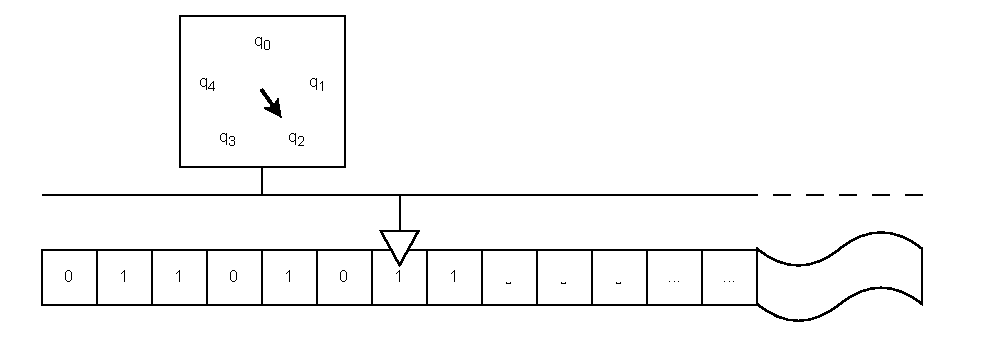
\includegraphics[scale=0.75]{resources/images/tm.pdf}

    \caption{A Turing machine}
\end{figure}

\newpage

\begin{definition}
 A Turing machine is a 7-uple $M = (Q, F, \Gamma, \Sigma, q_0, \delta)$ where:
    \begin{itemize}
        \item $Q$ is a finite set of states, $F \subseteq Q$ is a finite set of halting states and $q_0 \in Q$ is the initial state taken by the machine.
        \item $\Gamma$ is a finite set of symbols, usually called the tape alphabet. The tape alphabet always contains the symbol $\blankchar\,$, i.e. the black tape cell symbol.
        \item $\Sigma$ is a finite set of symbols, usually called the input alphabet, where $\Sigma \subseteq \Gamma - \{\blankchar\}$. The input string can be formed only of these characters.
        \item $\delta : (Q - F) \times \Gamma \to Q \times \Gamma \times \{\mathsf{L}, \mathsf{R}\}$ is a partial function, usually called the transition function, where $\mathsf{L}$ and $\mathsf{R}$ represents a left or right shift of the read-write head. Intuitively, if $\delta(q, a) = (p, b, L)$ then, when the machine is in state $q$ and reads the symbol $a$ on the current cell of the tape, it transitions to the state $p$, replaces the symbol $a$ with $b$ and moves the head to the left.
    \end{itemize}
\end{definition}

Turing \cite{turing} showed that a function can be computed by his theoretical machine if and only if it is lambda-computable, proving that the two models are equivalent. Turing's characterization of computation was acclaimed by Gödel himself, who deemed it \say{an absolute definition of an interesting epistemological notion}. The computational characterizations devised by Church and Turing would later be referred to as the \textbf{Church-Turing thesis}, constituting a formal definition of algorithm and computation.

Moreover, Turing proved the existence of an \textit{Universal Turing machine}, a \TM that is capable of simulating any other Turing machine. In other words, an \textsf{UTM} is capable of computing any function computable by another Turing machine. This result shouldn't be a surprise: modern computers are nothing more than a \textsf{UTM}s that can execute any given algorithm, producing an output for a given input.

The concept of Universal Turing machine also allows us to easily prove that many other computational models are capable of characterizing computation: if a model is capable of simulating an \textsf{UTM} then it is capable of making any possible computation. This idea is known as \textit{Turing completeness}.

After achieving a mathematically stable definition of computation through Turing machines, Church and Turing's focus shifted to understanding which problems are computable. In particular, they showed that some functions are \textbf{uncomputable} by proving that there cannot exist a Turing machine capable of carrying out their computation without going in infinite loops, i.e. never halting and thus never finding a solution. The main example of such a problem is Turing's famous \textit{Halting problem} which asks \say{does the given machine halt or not for a given input?}. Turing's proof is based on Cantor's \textit{diagonal argument}, a technique first used to show the non-numerability of the real numbers.

The existence of uncomputable functions - and thus uncomputable problems - gives a negative answer to the \textit{Entscheidungsproblem} (german for \textit{decision problem}), a question posed by David Hilbert in 1928 which asks if there is an algorithm that for each input statement answers \curlyquotes{yes} or \curlyquotes{no} according to whether or not the statement is universally true.

\newpage

\section{Complexity measures}

Once the existence of the absolute limits of computation was discovered, researchers shifter their focus on the \curlyquotes{practical} limits of computation. A \curlyquotes{good} algorithm (or \TM) should be able to solve a problem, in an efficient way. But what does it mean for a computation to be \textit{efficient}? To formally describe this idea, computer scientists defined \textbf{complexity measures} to quantify the amount of computational resources needed by a Turing machine. An efficient \TM should be able to solve a task with low computational resources. Above all, we are interested in studying the amount of steps needed and the amount of cells needed to achieve such computations. These two concepts are referred to as the \textit{time complexity} and the \textit{space complexity} of a Turing machine.

\begin{definition}
 Given a Turing machine $M$ that halts on every input, we define the time complexity and space complexity of $M$ as the two functions $t, s : \N \to \R^+$ such that $t(n)$ and $s(n)$ are respectively the maximum number of steps and cells used by $M$ during the computation for any input of length $n$.
\end{definition}

Even between small powers there is a huge difference in resources. For instance, an algorithm that requires $n$ steps is clearly a lot more efficient than one that requires $n^2$ steps. In complexity theory, we consider as \textbf{efficient} any solution that requires a \curlyquotes{reasonable} amount of resources, even when they are huge: an algorithm that requires $n^{1000}$ steps is still considered \curlyquotes{reasonable}, while the same doesn't hold for an algorithm that requires $2^n$ steps. In other words, efficiency dictates whether a problem is feasible or not in the real world: if a problem is computable by a \TM but it requires an immense amount of time or space to get to the result, then the computation is practically unachievable. These problems are often referred to as \textbf{intractable problems} \cite{complexity_arora_barak,sipser_computation}.

Time and space complexity are intrinsically related one to the other. For instance, if a machine has time complexity $t(n)$ then the number of cells that can be used is limited by $t(n)$, hence $s(n) \leq t(n)$. Usually, these two measures are proportionally inverse: if we allow our algorithm to use more space then the computation can be sped up, while if we want to lower the amount space needed then the computation will require more steps. Larger inputs require a larger amount of computational resources, making the values $t(n)$ and $s(n)$ proportional to the size $n$ of the input. For this reason, as the input size grows, we are interested in the asymptotic behavior of these measures. This concept is captured by the so-called \textit{big-Oh notation}.

\begin{definition}
 Given two functions $f, g : \N \to \R^+$, we say that:
    \begin{enumerate}
        \item $f$ is in big-Oh of $g$, written as $f(n) = O(g(n))$, if there are two constants $c \in \R$ and $N \in \N_{> 0}$ such that $\forall n \geq N$ it holds that $f(n) \leq c g(n)$.
        \item $f$ is in Omega of $g$, written as $f(n) = \Omega(g(n))$, if there are two constants $c \in \R$ and $N \in \N_{> 0}$ such that $\forall n \geq N$ it holds that $f(n) \geq c g(n)$.
        \item $f$ is in Theta of $g$, written as $f(n) = \Theta(g(n))$, iif there are two constants $c \in \R$ and $N \in \N_{> 0}$ such that $\forall n \geq N$ it holds that $c g(n) \leq f(n) \leq d g(n)$.
    \end{enumerate}
\end{definition}

In other words, as the input size $n$ grows the function $f$ can dominate, be dominated or both by a function $g$, defining the \textit{lower} and \textit{upper} bounds of the value $f(n)$. In particular, when $f(n) = \Theta(g(n))$ the two functions can be considered to be \textit{almost} the same due to them following the same growth pattern. Additionally, its easy to see that $f(n) = \Omega(g(n))$ if and only if $g(n) = O(f(n))$ and likewise that $f(n) = \Theta(g(n))$ if and only if $f(n) = O(g(n))$ and $f(n) = \Omega(g(n))$.

In general, we consider an algorithm as \textit{time efficient} if it can compute the answer to any input in at most a polynomial amount of time, i.e. in $O(n^k)$ time for some $k \in \N$. Likewise, it is considered \textit{space efficient} if it can compute the answer to any input in at most a polynomial amount of space.

For example, consider the following informally defined Turing machine $M$ which takes the binary encoding $\abk{m}$ of a natural number $m \in \N$ as the input string and returns $\abk{m^2}$ as the output string. The computation made by $M$ is achieved by repeatedly adding the value $m$.

\noindent
$M$ = "Given the input string $\abk{m}$:
\begin{enumerate}
    \item Copy the string $\abk{m}$ on a blank set of contiguous cells. This copied string will be referred to as the value $k$.
    \item Copy the string $\abk{m}$ on a blank set of contiguous cells. This copied string will be referred to as the value $y$.
    \item Repeat while the value $k$ is bigger than $1$:
    \begin{enumerate}[label={\arabic*.}, start=3]
        \item Copy the string $\abk{y}$ on a blank set of contiguous cells. This copied string will be referred to as the value $x$.
        \item Compute $x + n$ and store the result on the space occupied by the string $\abk{y}$. In other words, compute $y \gets x + n$.
        \item Compute $k - 1$ and store the result on the space occupied by the string $\abk{k}$. In other words, compute $k \gets k - 1$.
    \end{enumerate}
\end{enumerate}
\begin{enumerate}[label={\arabic*.}, start=6]
    \item Write $\blankchar$ on all the cells on the tape, except for the cells of the string $\abk{o}$.
    \item Halt the machine and return the output string $\abk{o}$."
\end{enumerate}

We know that any natural number $m \in \N$ can be encoded in binary with $\log_2 m$ bits. This means that the length $n$ of the input string $\abk{m}$ is $\log_2 m$.

Consider now the values $k$ and $o$ obtained in the computation. These values are natural numbers and they are bounded by $cm$ for some $c \in \R$. This means that $k, x, y = O(m)$ and thus that they can be encoded with $O(\log m)$ bits (asymptotic notation allows us to drop the subscript of the logarithm), therefore requiring $3 \cdot O(\log m)$ cells, which is asymptotically equivalent to $O(\log m)$ cells. We conclude that the space complexity of our \TM is $O(\log m) = O(n)$.

To copy a string of length $\ell$, the Turing machine needs to copy $\ell$ cells but also requires to make additional shifts in order to repeatedly move from the original string to the copied one, making the total amount of steps required $O(\ell)$. In a similar fashion, binary addition (or subtraction) between two numbers $a$ and $b$ can be computed in $O(\log a + \log b)$ steps. Since we initially set $k = m$ and the machine decrements the value of $k$ by 1 on each iteration of the loop, the computations inside the loop get executed $m-1$ times. This means that the total number of loop steps is $O((m-1) \log m)$. By adding the initial two copy procedures, the total number of steps done by the machine is $O(2 \log m + (m-1) \log m)$, which is asymptotically equivalent to $O(m \log m)$. Thus, we conclude that the time complexity of such $\TM$ is $O(m \log m) = O(2^n n)$.

These complexity measures clearly imply that this \TM is highly time inefficient since it requires an exponential amount of time. But does this mean that the problem is intractable? Modern computers can square a number in milliseconds, so the answer to this question should clearly be no. In fact, even by implementing the common column method for multiplying numbers usually taught to kids, this problem can be solved efficiently.

Efficiency is one of the lingering question in modern computer scientists. We know that some problems are computationally unattainable, but where is the line that separates tractable and intractable problems? What property defines problems that cannot be solved efficiently? Finding an answer to these questions may seem easy, but after more than 70 years of research it still persists in the minds of complexity theorists.


\chapter{Search problems} \label{chap:search_problems}

\section{Decision vs. Search}

For many years, the study of \textbf{decision problems} has been the main focus of computability theory. These problems can be described as simple questions with a \say{yes} or \say{no} answer, such as asking if some input object has some property or not. Given a language $\Sigma^*$, where $\Sigma$ is an alphabet of symbols and $\Sigma^*$ is the set of all strings on $\Sigma$, each decision problem can be described as a subset of $\Sigma^*$, where a string $\abk{o}$ that encodes an object $o$ is in the subset if and only if the answer to the problem for that object is positive. A \say{yes} answer is represented by a 1, while a \say{no} answer is represented by a 0. For example, given the language $\N$, the question \say{is $n$ a prime number?} is modeled by the decision problem $\mathrm{PRIMES} = \{n \in \N \mid n \text{ is prime}\}$. Since any symbol of an alphabet $\Sigma$ can be encoded as an unique sequence of bits, we can assume that $\{0,1\}$ is our unique alphabet of interest \cite{complexity_arora_barak,sipser_computation}.

\begin{definition}
 A decision problem for a property $P$ is a subset $L$ of a language $\{0,1\}^*$ such that $L = \{x \in \{0,1\}^* \mid P(x) = 1\}$.
\end{definition}

A decision problem is said to be \textit{decidable} if there is a Turing machine answers the question posed by the problem with 0 or 1 for any input $x \in \{0,1\}^*$. This also implies that the machine has to halt for every input. Decidability theory plays a large role in mathematics and computer science since most problems can be modeled through it. However, by their nature, decision problems are limited. Some problems require a more complex result than a simple yes-or-no answer. Instead of asking the question \say{does this object have the required property?}, we may be more interested in the question \say{what gives this object the following property?}.

These kinds of questions are modeled by \textbf{functional problems}, i.e. any problem where an output that is more complex than a yes-or-no answer is expected for a given input. Functional problems are by nature \curlyquotes{harder} than decision problems, describing any possible type of computation achievable through the concept of computable function, even decidability itself (any decision problem is just a functional problem with only two possible outputs).

\newpage

Functional problems are described through the concept of relation: given a set of inputs $X$ and a set of possible outputs $Y$, a functional problem is as a relation $R \subseteq X \times Y$ such that the pair $(x,y)$ is in $R$ if and only if $y$ is the output to the input $x$ for the given question. For instance, the question \say{what is the prime factorization of $n$?} is modeled by the functional problem $\mathrm{FACTOR} = \{(n, (p_1, \ldots, p_k)) \in \N \times \N^k \mid n = p_1 \cdot \ldots \cdot p_k\}$.

We observe that questions like \say{is $y$ a valid output for the input $x$?} are still modeled by decision problems due to them requiring a simple yes-or-no answer, while a function problem would ask the question \say{what is the output for the input $x$?}. For example, the question \say{is $p_1, \ldots, p_k$ the prime factorization of $n$?} corresponds to the decision problem $\mathrm{FACTORIZATION}_n = \{(p_1, \ldots, p_k) \in \N^k \mid n = p_1 \cdot \ldots \cdot p_k\}$.

Even though decision problems can indeed be modeled as functional problems whose outputs are only \say{yes} and \say{no}, they aren't effectively a subset of functional problems due to them being defined differently: the decision problem $\mathrm{PRIMES}$ can be converted into the functional problem $\{(n, b) \in \N \times \{0,1\} \mid b = 1 \text{ if } n \text{ is prime, } b = 0 \text{ otherwise}\}$, but they aren't effectively the same problem despite answering the same question.

Another important thing to notice is that, even though the name implies a correlation to standard mathematical functions due to the concept of input-output being involved, the given definition also includes \textit{partial} and \textit{multivalued} functions, i.e. functions for which not all inputs have a corresponding output and functions for which one input can have more outputs. For these reasons, the term \textit{functional problem} is considered to be slightly abused. In recent years, this issue was solved by the introduction of the more general term \textbf{search problems}, describing the idea of finding a valid output for the given input, better suiting the previous formal definition.

To give a more detailed definition of search problems, we assume that these problems all share the language $\{0,1\}^*$, describing all inputs as a sequence of bits. Since each problem could have inputs of different lengths, researchers have defined search problems through the use of a sequence of relations rather than a single relation \cite{rel_comp_np_search, proofs_circuits_communication, tfnp_characterization}. This also allows separation between different types of outputs based on the length of the inputs.

\begin{definition}
 A search problem is a sequence $R = (R_n)_{n \in \N}$ of relations $R_n \subseteq \{0,1\}^n \times O_n$, one for each $n \in \N$, where each $O_n$ is a finite set called outcome set.
\end{definition}

Since it includes partial functions, this definition allows search problems to be \curlyquotes{undefined} for some inputs, meaning that there is no answer for some inputs. A search problem is said to be \textbf{total} if for each $R_n$ in the sequence it holds that $\forall x \in \{0,1\}^n$ there is an answer $y \in O_n$ such that $(x,y) \in R_n$. In other words, a total search problem has at least an output for all possible inputs, removing partial functions from the context, while multivalued functions are still allowed. For example, $\mathrm{FACTORING}$ is a total non-multivalued search problem due to each natural number having a guaranteed unique prime factorization by the Fundamental Theorem of Arithmetic.

\newpage

\section{The complexity classes \textsf{FP}, \textsf{FNP} and \textsf{TFNP}}

In complexity theory, decision problems are grouped into numerous categories, each defining a subclass. The most important subclass corresponds to the set of problems that can be \textbf{efficiently solved}. This class is referred to as \textsf{P}, i.e. the class of problems solvable by a Turing machine in polynomial time. Not all decision problems are efficiently solvable, i.e. the so-called \textit{intractable problems} (see \Cref{chap:introduction}). Several problems for which there is currently no answer regardless of whether or not they are efficiently solvable have been shown to be \textbf{efficiently verifiable}, meaning that there is a Turing machine called \textit{verifier} that given an additional input $c$, namely the \textit{certificate}, is capable of telling in polynomial time if the value $y$ is the output of an input $x$.

\begin{definition}
 A verifier for a decision problem $L$ is a Turing machine $V$ such that for each input $x \in \Sigma^*$ there is a certificate $c \in \Sigma^*$ for which $V(x,c) = 1$ if and only if $x \in L$.
\end{definition}

The class of problems that are verifiable by a polynomial time verifier with certificates of polynomial length is referred to as \textsf{NP}. This class is equivalent to the class of problems efficiently solvable by a \textit{non-deterministic Turing machine}, a \TM that on each step of the computation can choose between a set of possible actions, branching the computation. Originally, the class \textsf{NP} was defined through this type of \TM \@ - hence the name of the class being an abbreviation for \textit{non-deterministic polynomial time} - but it quickly got replaced with the verifier definition due to \textsf{NTM}s being only a theoretical computational model that is physically unrealizable \cite{complexity_arora_barak}. For our purposes, we will consider the modern definition of \textsf{NP}.

\begin{definition}
    We define $\mathsf{P}$ as the set of decision problems that can be solved by a polynomial time \TM. We define $\mathsf{NP}$ as the set of decision problems that can be verified by a polynomial time verifier.
\end{definition}

It's easy to see that $\mathsf{P} \subseteq \mathsf{NP}$ since every efficiently solvable problem can also be efficiently verified by simply ignoring the certificate and solving the problem. However, it is currently not known whether $\mathsf{P} = \mathsf{NP}$ or not. The answer to this question is considered to be one of the most important questions in mathematics. In fact, if $\mathsf{P} = \mathsf{NP}$ were to be true, a lot of key problems in mathematics that are currently only efficiently verifiable could be solved in a reasonable amount of time by a modern computer. On the other hand, a large number of current technologies are based on the assumption that $\mathsf{P} \neq \mathsf{NP}$. Examples include the field of cryptography, which assumes that it's easy to check that each encrypted string is the result of the encryption scheme being applied to the original message, which works as the certificate, and very hard to find this message only through the encrypted string. If $\mathsf{P} \neq \mathsf{NP}$ were proven false, we would have to reconsider a large portion of the modern world, even digital currencies themselves.

In the context of search problems, we define the class \textsf{FP} - \textit{functional} \textsf{P} - as the class of search problems efficiently solvable by an algorithm and \textsf{FNP} - \textit{functional} \textsf{NP} - as the class of search problems whose solutions are efficiently verifiable by a verifier. 

\newpage

\begin{definition}
 We define $\mathsf{FP}$ as the set of search problems $R = (R_n)_{n \in \N}$ whereby $\forall n \in \N$ there is a polynomial time \TM $T_n$ such that $T_n(x) = y$ if and only if $(x,y) \in R_n$. We define $\mathsf{FNP}$ as the set of search problems $R = (R_n)_{n \in \N}$ whereby $\forall n \in \N$ there is a polynomial time verifier $V_n$ such that $\exists w \in \{0,1\}^{n^k}$ for which $V_n(x,y,w) = 1$ if and only if $(x,y) \in R_n$. 
\end{definition}

An important remark to be made is that, even though any decision problem can be transformed into a search problem with only two possible outputs, since they are defined on two different types of problems it doesn't make sense to say that \textsf{P} $\subseteq$ \textsf{FP} or that \textsf{NP} $\subseteq$ \textsf{FNP}. However, an important result shows that it can hold that $\textsf{P} = \textsf{NP} $ if and only if $\textsf{FP} = \textsf{FNP}$ \cite{decision_vs_search, fp_vs_p}. This implies that, despite search problems being by definition more complex than decision problems, the functional version of the conjecture is as hard as the decisional one.

\begin{theorem}
    $\textsf{P} = \textsf{NP}$ if and only if $\textsf{FP} = \textsf{FNP}$
\end{theorem}

\begin{proof}
 Since each decision problem can be translated into a search problem with only two possible outcomes, we trivially get that if $\textsf{FP} = \textsf{FNP}$ then $\textsf{P} = \textsf{NP}$.
    
 Suppose now that $\textsf{P} = \textsf{NP}$. We already know that $\textsf{FP} \subseteq \textsf{FNP}$, so we have to show that $\textsf{FP} \subseteq \textsf{FNP}$. Let $R = (R_n)_{n \in \N} \in \textsf{FNP}$ be a search problem verifiable in polynomial time.
    
 For each $n \in \N$, let $L_n$ be the set of pairs $(x,z)$ such that $z$ is the prefix of an outcome $zw$ for the problem $R_n$ with input $x$, formally $L_n = \{(x,y) \mid \exists z \in \{0,1\}^{k}, k \leq n \text{ s.t. } (x,zw) \in R_n\}$. It's easy to see that $L_n \in \textsf{NP}$ since each pair $(x,z)$ is certified by the string $zw$ itself and the correctness of this certificate can be polynomially verified given that $R \in \textsf{FNP}$.
    
 Since $L_n \in \textsf{NP} = \textsf{P}$, we know that there is a polynomial time algorithm $\mathrm{Partial}_n$ that decides $L_n$. Thus, for each $n \in \N$, we can construct the following polynomial time algorithm $\mathrm{Solve}_n$ which directly concludes that $R \in \textsf{FP}$ and thus that $\textsf{FNP} \subseteq \textsf{FP}$.

    \begin{algorithmic}
        \Function{$\mathrm{Solve}_n$}{$x$}
            \State{$y$ = $\varepsilon$}
            \Comment{$\varepsilon$ is the empty string}
            \While{True}
                \If{$\mathrm{Partial}_n(x,y0)$ = True}
                    \State{$y$ = $y0$}
                \ElsIf{$\mathrm{Partial}_n(x,y1)$ = True}
                    \State{$y$ = $y1$}
                \Else
                    \State{return $y$}
                \EndIf
            \EndWhile
        \EndFunction
    \end{algorithmic}
\end{proof}

\newpage

As discussed in the previous section, not all search problems are total, meaning that a solution could not exist for some inputs. A lot of real-world problems have a guaranteed solution for each input, ranging from simple number functions to harder problems, making total search problems more interesting than non-total ones.

\begin{definition}
 We define the class $\mathsf{TFNP}$ as the subset of \textsf{FNP} problems that are also total.
\end{definition}

For simplicity, we assume that each search problem in \textsf{FP} is also total: since problems in \textsf{FP} are solvable in polynomial time, when a solution doesn't exist we can output a pre-chosen \say{doesn't exist} solution, making the problem total. This assumption easily implies that \textsf{FP} $\subseteq$ \textsf{TFNP} $\subseteq$ \textsf{FNP}, giving us a proper hierarchy. For natural reasons, this assumption wouldn't work for \textsf{FNP} problems: the only way to polynomially verify that a solution doesn't exist would be to solve the problem itself and find that there is no solution, implying that \textsf{FP} = \textsf{FNP} would be trivially true.

Another way to view total search problems is through the lens of \textit{polynomial disqualification}. In decisional problems, the class \textsf{coNP} contains all the problems whose complement is in \textsf{NP}. If the complementary problem is polynomially verifiable, this means that there is a polynomial verifier that can decide if an input doesn't have the required property, effectively disqualifying it. Proving that a decision problem is in \textsf{coNP} is also equivalent to proving that for each input of that problem there is no string capable of certifying that the solution is correct. Researchers currently believe that $\mathsf{NP} \neq \mathsf{coNP}$, even though this is still an open question. If the answer to this question is proven negative, we would also have a direct answer to the $\mathsf{P} \stackrel{?}{=} \mathsf{NP}$ question: we know that if $\mathsf{NP} \neq \mathsf{coNP}$ then $\mathsf{P} \neq \mathsf{NP}$ \cite{complexity_arora_barak, sipser_computation}

For search problems, we define the class \textsf{FcoNP} in the same way. In particular, the class $\textsf{TFNP}$ corresponds to the class $\mathsf{F}(\mathsf{NP} \cap \mathsf{coNP})$, which contains search problems whose inputs can be certified and disqualified in polynomial time \cite{tfnp_f_np_conp}.

\begin{proposition}
    \label{tfnp_f_np_conp}
    $\mathsf{TFNP} = \mathsf{F}(\mathsf{NP} \cap \mathsf{coNP})$
\end{proposition}

\begin{proof}
 If $R = (R_n)_{n \in \N} \in \textsf{TFNP}$ then we know that every input $x$ has an output $y$. However, this means that the complementary problem $\overline{R}$ is empty, meaning that each input is trivially verifiable in polynomial time and thus that $\overline{R} \in \textsf{FNP}$. Hence, we conclude that $R \in \mathsf{F}(\mathsf{NP} \cap \mathsf{coNP})$.
    
 Vice versa, if $S \in \mathsf{F}(\mathsf{NP} \cap \mathsf{coNP})$ then trivially we have that $S \in \mathsf{FNP}$. Moreover, since $S \in \mathsf{F}(\mathsf{NP} \cap \mathsf{coNP})$ we know that each input $x$ can be easily certified or disqualified in polynomial time, meaning that each input must have a solution polynomially verifiable and thus that $S \in \mathsf{TFNP}$.

\end{proof}

\newpage

\section{Reductions between problems}

One of the most interesting aspects of computable (and uncomputable) problems is the ability to be transformed into another problem in order to achieve a solution. Suppose that we have an instance $a$ of problem $A$ and that we know an algorithm that transforms $a$ into an instance $b$ of a problem $B$ such that $a$ is a \say{yes} answer if and only if $b$ is a \say{yes} answer. Then, by solving $b$ we would get an answer to $a$. In computer science, this concept is known as \textbf{reduction}: a problem $A$ is said to be reducible into a problem $B$, written as $A \leq B$, if any instance $a$ of $A$ can be mapped into an instance $b$ of $B$ whose solution gives a solution to the former.

In decision problems, this concept is described through \textit{many-to-one mappings}, computable functions that map instances of the original problem to instances of the reduced problem.

\begin{definition}
 A decision problem $A$ is many-to-one reducible to a decision problem $B$, written as $A \leq_m B$, if there is a computable function $f$ such that $x \in A$ if and only if $f(x) \in B$. 
\end{definition}

To better understand how reductions work, consider the $3\mathrm{COL}$ problem, which asks the question \say{is this graph 3-colorable?}. A graph is said to be 3-colorable if we can color each node of the graph with a color different from all of its neighbors by using at most 3 colors.

\begin{figure}[H]
    \centering
    
    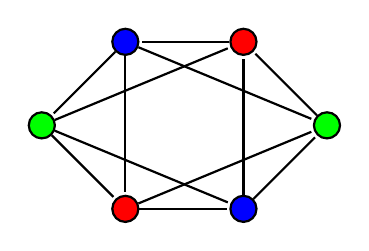
\begin{tikzpicture}[-,>=stealth,shorten >=1pt,auto,node distance=1.5cm, thick,main node/.style={scale=0.9,circle,draw,font=\sffamily\normalsize}]
    
        \node[circle, draw, fill=blue] (1) []{};
        \node[circle, draw, fill=green] (2) [below left of=1]{};
        \node[circle, draw, fill=red] (3) [below right of=2]{};
        \node[circle, draw, fill=blue] (4) [right of=3]{};
        \node[circle, draw, fill=green] (5) [above right of=4]{};
        \node[circle, draw, fill=red] (6) [above left of=5]{};
    
        \path[every node/.style={font=\sffamily\small}]
            (1) edge (2)
            (2) edge (3)
            (3) edge (4)
            (4) edge (5)
            (5) edge (6)
            (6) edge (1)

            (1) edge (3)
            (1) edge (5)
            (2) edge (6)
            (2) edge (4)
            (3) edge (5)
            (4) edge (6)

            ;
    \end{tikzpicture}
    
    \caption{Example of a 3-colorable graph}
\end{figure}

This problem can easily be reduced to the $\mathrm{SAT}$ problem, which asks the question \say{does this propositional formula have an assignment that satisfies it?}. This problem is clearly in \textsf{NP}: if $\phi$ is a satisfiable formula, we can use an assignment $\alpha$ that satisfies $\phi$ as the certificate, which can easily be done in linear time. To reduce $3\mathrm{COL}$ to $\mathrm{SAT}$, we construct the following sub-formulas:
\begin{itemize}
    \item For each node $v \in V(G)$, we define the sub-formula $\phi_v = (r_v \lor g_v \lor b_v)$ which imposes that each node must have at least one color assigned
    \item For each edge $(u,v) \in E(G)$, we define the sub-formula $\phi_{(u,v)} = (\overline{r_u} \land \overline{r_v}) \land (\overline{g_u} \land \overline{g_v}) \land (\overline{b_u} \land \overline{b_v})$ which imposes that the nodes of each edge must have different colors.
\end{itemize}

Then, we construct the final formula that encodes the 3-colorization of $G$:
\[\phi_G = \left ( \bigwedge_{v \in V(G)} \phi_v \right ) \land \left ( \bigwedge_{(u,v) \in E(G)} \phi_{(u,v)} \right )\]

By definition of $\phi_G$, it holds that $G$ is 3-colorable if and only if $\phi_G$ is satisfiable. In particular, there is a bijection between $G$'s color assignments and $\phi_G$'s variable assignments. This concludes that $3\mathrm{COL} \leq_m \mathrm{SAT}$. Moreover, this reduction can be computed by a Turing machine in polynomial time. When this happens, we say that $3\mathrm{COL} \leq_p \mathrm{SAT}$

Many-to-one reductions between problems are transitive: starting from a problem $A$, we can reduce it to a problem $B$ through a function $f$ and then reduce it to a problem $C$ through a function $g$. This implies that the composition $g \circ f$ is a reduction from $A$ to $C$. For instance, the $\mathrm{4\text{-}COL}$ problem, a variant of the $\mathrm{3\text{-}COL}$ with four colors instead of three colors, can be reduced in polynomial time to $\mathrm{3\text{-}COL}$, giving us the reduction chain $\mathrm{4\text{-}COL} \leq_p \mathrm{3\text{-}COL} \leq_p \mathrm{SAT}$.

Reductions between decision problems map any \say{yes} answers of problem $A$ to some \say{yes} answers of problem $B$ and the same goes for \say{no} answers. In search problems, however, there is no concept of a negative answer: even if a problem has only two possible outputs, both of them are still a solution. Some people could argue that an input for which there is no solution is a negative answer to the search problem. But how could we map inputs without solutions to other inputs without solutions? What if one of the two problems involved is total and the other isn't? This clearly doesn't make sense and, even if it did, we are only interested in finding solutions. We give the following definition of search problem reduction:

\begin{definition}
 A search problem $R = (R_m)_{m \in \N}$, where $R_m \subseteq \{0,1\}^m \times O_m$ is said to be many-to-one reducible to a search problem $S = (S_n)_{n \in \N}$, written as $R \leq_m S$, where $S_n \subseteq \{0,1\}^n \times O_n'$, if for all $m \in \N$ there is an $n \in \N$ for which there is a computable function $f : \{0,1\}^m \to \{0,1\}^n$ and a computable function $g : \{0,1\}^m \times O_n' \to O_m$ such that:
    \[\forall x \in \{0,1\}^m \;\; (f(x), y) \in S \implies (x, g(x,y)) \in R\]
 In other words, the function $f$ maps inputs of $R$ into inputs of $S$, while the function $g$ maps solutions of $S$ into solutions of $R$. 
\end{definition}

When a reduction can be efficiently computed by a \TM with a time (or space) complexity that is in the order of to the complexity of $B$, the problem $A$ can be solved by a machine that first computes the reduction and then solves the problem $B$. For instance, if $A \leq_p B$ through a function $f$ and $B$ can be solved in polynomial time then we can build a machine that first computes $f(x)$ for a given input $x$ and then compute whether $f(x) \in B$ or not. Since both the reduction and the final computation in this case require polynomial time, we conclude that $A$ can also be solved in polynomial time.

Reductions play a critical role in computer science. In particular, they allow us to define the concept of \textbf{completeness}. A problem is considered complete for a class $\mathcal{C}$ when every problem from its class can be reduced to it under a specific constraint. This constraint usually depends on the complexity constraints dictated by a subclass $\mathcal{D} \subseteq \mathcal{C}$: if every problem in $\mathcal{C}$ is reducible to $B$ under the same constraints that define the subclass $\mathcal{D}$ and we can show that $B \in \mathcal{D}$, then the whole class $\mathcal{C}$ collapses onto its subclass, that is $\mathcal{C} = \mathcal{D}$.

For instance, since $\mathsf{P} \subseteq \mathsf{NP}$, the completeness constraint behind \textsf{NP}-Completeness would be to maintain polynomial time reductions. In \textsf{P}-Completeness, instead, the completeness constraint would be to maintain logarithmic space reductions due to how $\mathsf{L} \subseteq \mathsf{P}$, where $\mathsf{L}$ is the class of problems decidable in logarithmic space.

\begin{definition}
    A problem $B$ is said to be \textsf{NP}-Complete if $B \in \mathcal{C}$ and $\forall A \in \mathsf{NP}$ it holds that $A \leq_p B$.
\end{definition}

From this definition, we derive that an \textsf{NP}-Complete problem can be solved in polynomial time if and only if $\mathsf{P} = \mathsf{NP}$. The $\mathrm{SAT}$ problem previously described is actually the first ever known \textsf{NP}-Complete problem, a seminal result proven by Cook in 1971 \cite{cook_sat} and later by Levin in 1973 \cite{levin_fsat}. In particular, Levin proved this result through the functional version of this complete problem $\mathrm{FSAT}$, which asks the question \say{which assignment satisfies the following formula?}, modeling what he called \textit{universal sequential search problem}. In fact, the functional versions can be used to prove that the decisional versions are complete and vice versa \cite{rel_comp_np_search}.

\begin{theorem}
 The decisional problem $A$ is \textsf{NP}-Complete if and only if the functional problem $FA$ is \textsf{FNP}-Complete.
\end{theorem}

Since Cook's result, many important problems have been shown to be \textsf{NP}-Complete, such as Karp's 21 decision problems \cite{karp}. Nowadays, thousands of problems fall into this class. Since most researchers believe that $\mathsf{P} \neq \mathsf{NP}$, once a problem is proven to be \textsf{NP}-Complete they start looking to approximations of the problem, due to a general optimal solution being out of reach. Proving that $\mathsf{P} \neq \mathsf{NP}$ would imply that all such problems are actually \textit{intractable}, making approximation algorithms the best we can hope for.

\section{The \textsf{TFNP} hierarchy}

Currently, it is not known if there is a \textsf{FNP}-Complete problem that is also \textit{total}. For example, the problem $\mathrm{FSAT}$ isn't total due to some formulas being unsatisfiable, thus no satisfying assignment can be returned as a solution. Researchers believe that the existence of such a problem is very unlikely. 

For these reasons, in the \textsf{TFNP} world the concept of completeness is studied under a \textit{different approach}: instead of considering problems that are complete for the whole class, we consider important problems that have a lot of \textsf{TFNP} problems reducible to them. These important problems form additional subclasses of \textsf{TFNP}. With a slight abuse of notation, we denote with $S$ the class of problems efficiently reducible to the search problem $S$.

\begin{definition}
 Given \textsf{TFNP} problem $S$, we define the class $S$ as the subset of \textsf{TFNP} problems efficiently reducible to the problem $S$ in polynomial time, formally $S = \{R \in \mathsf{TFNP} \mid R \leq_m S \text{ in polynomial time}\}$
\end{definition}

The extensive study of \textsf{TFNP} classes has been successful in capturing the complexity of many branches of mathematics, such as problems from cryptography, game theory and economics that are reducible to TFNP complete problems. Unexpectedly, a vast majority of total search problems can be characterized with very few subclasses, which form the \textbf{\textsf{TFNP} hierarchy}. 

\newpage

Each of these subclasses is characterized by a complete total search problem that describes an elementary question, such as determining if a mapping doesn't have collision or not - or equivalently, if a function is injective or not \cite{proofs_circuits_communication,tfnp_characterization}. These complete problems are guaranteed to be total by the very \textit{combinatorial principles} that dictate them:

\begin{itemize}
    \item \textsf{PLS} (Polynomial Local Search): the class of search problems designed to model the process of finding the local optimum of a function or the class of problems whose solution is guaranteed by the \say{Every directed acyclic graph has a sink} principle. It is formally defined as the class of search problems that are polynomial-time reducible to the SINK-OF-DAG problem.
    
    \item \textsf{PPP} (Polynomial Pigeonhole Principle): the class of problems whose solution is guaranteed by the \say{Every mapping from a set of $n+1$ elements to a set of $n$ elements has a collision} principle. It is defined as the class of problems that are polynomial-time reducible to the PIGEON problem.
    
    \item \textsf{PPA} (Polynomial Parity Argument): the class of problems whose solution is guaranteed by the \say{Every undirected graph with an odd-degree node must have another odd-degree node} principle. It is defined as the class of problems that are polynomial-time reducible to the LEAF problem.
    
    \item \textsf{PPADS} (Polynomial Parity Argument - Directed with Sink): the class of problems whose solution is guaranteed the \say{Every directed graph with a positively unbalanced node (out-degree > in-degree) must
 have a negatively unbalanced node} principle. It is defined as the class of problems that are polynomial-time reducible to the SINK-OF-LINE problem.
    
    \item \textsf{SOPL} (Sink of Potential Line): the class of problems that are polynomial-time reducible to the SINK-OF-POTENTIAL-LINE problem. It has been proven that $\mathsf{SOPL} = \mathsf{PLS} \cap \mathsf{PPADS}$ \cite{Further_collapses_TFNP}
    
    \item \textsf{PPAD} (Polynomial Parity Argument - Directed): the class of problems whose solution is guaranteed the \say{Every directed graph with an unbalanced node must have another unbalanced node} principle. It is defined as the class of problems that are polynomial-time reducible to the END-OF-LINE problem.
    
    \item \textsf{CLS} (Continuous Local Search): the class of search problems designed to model the process of finding a local optimum of a continuous function over a continuous domain. It is defined as the class of problems that are polynomial-time reducible to the CONT-LOCALPOINT problem. It has been proven that $\mathsf{CLS} = \mathsf{EOPL} = \mathsf{PLS} \cap \mathsf{PPAD}$ \cite{gradient_descent, Further_collapses_TFNP}, where \textsf{EOPL} is the class of search problems that are polynomial-time reducible to the END-OF-POTENTIAL-LINE problem.
\end{itemize}

\newpage

\begin{figure}[H]
    \centering
    
    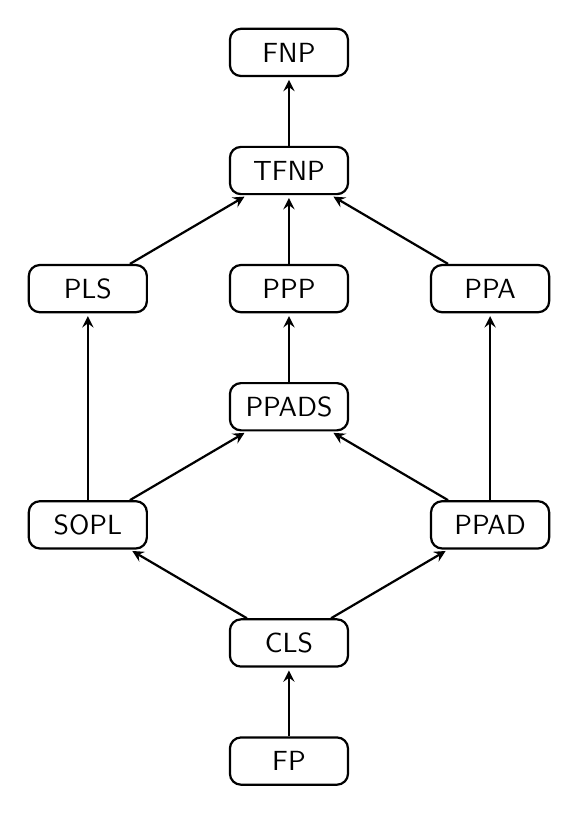
\begin{tikzpicture}[->,>=stealth,shorten >=1pt,auto,node distance=1.5cm, thick,main node/.style={scale=0.9,circle,draw,font=\sffamily\normalsize}]
    
        \node[rectangle, draw, rounded corners, minimum width=15mm, minimum height=6mm] (1) []{\textsf{FNP}};

        \node[rectangle, draw, rounded corners, minimum width=15mm, minimum height=6mm] (2) [below of = 1]{\textsf{TFNP}};

        \node[rectangle, draw, rounded corners, minimum width=15mm, minimum height=6mm] (3) [below of = 2]{\textsf{PPP}};

        \node[rectangle, draw, rounded corners, minimum width=15mm, minimum height=6mm] (4) [left of = 3, xshift=-30]{\textsf{PLS}};

        \node[rectangle, draw, rounded corners, minimum width=15mm, minimum height=6mm] (5) [right of = 3, xshift=30]{\textsf{PPA}};

        \node[rectangle, draw, rounded corners, minimum width=15mm, minimum height=6mm] (6) [below of = 3]{\textsf{PPADS}};

        \node (7) [below of = 6]{};

        \node[rectangle, draw, rounded corners, minimum width=15mm, minimum height=6mm] (8) [left of = 7, xshift=-30]{\textsf{SOPL}};

        \node[rectangle, draw, rounded corners, minimum width=15mm, minimum height=6mm] (9) [right of = 7, xshift=30]{\textsf{PPAD}};

        \node[rectangle, draw, rounded corners, minimum width=15mm, minimum height=6mm] (10) [below of = 7]{\textsf{CLS}};

        \node[rectangle, draw, rounded corners, minimum width=15mm, minimum height=6mm] (11) [below of = 10]{\textsf{FP}};
    
        \path[every node/.style={font=\sffamily\small}]
            (2) edge (1)
            (3) edge (2)
            (4) edge (2)
            (5) edge (2)
            (6) edge (3)
            (8) edge (4)
            (8) edge (6)
            (9) edge (5)
            (9) edge (6)
            (10) edge (8)
            (10) edge (9)
            (11) edge (10)
            ;
    \end{tikzpicture}
    
    \caption{Hierarchy of the main total search problem subclasses. \\ An arrow from class $A$ to class $B$ means that $A \subseteq B$.}
\end{figure}

Interestingly, lots of complex problems have been proven to be reducible to these basic problems. For example, the $\mathrm{NASH}$ problem relative to finding a Nash equilibrium of a given game has been shown to not only lie inside \textsf{PPAD} but also be \textsf{PPAD}-Complete \cite{nash_1, nash_2}. One should ponder what it really means for a problem to be complex.

Proving any unconditional separation between these subclasses, which can be achieved by showing that one of them is not efficiently reducible to the other, would directly imply that $\mathsf{FP} \neq \mathsf{TFNP}$, answering the $\mathsf{P} \stackrel{?}{=} \mathsf{NP}$ question. By the hardness of the question itself, finding such unconditional separation seems to be completely out of reach. However, it turns out that the \textsf{TFNP} model indeed has conditional separations, in particular relative to \textit{oracles} (see \Cref{chap:bb-tfnp}).
 
\newpage

\section{White-box \textsf{TFNP}}

In computer science and engineering, systems and models are distinguished between white-box and black-box systems. A system is \textbf{white-box} if its internal workings are known, meaning that given any input it is possible to know how the system achieves a result. Contrary, the computational process is unknown in a \textbf{black-box} system. Black-box models allow us to consider only the result for a given input, ignoring how that result is achieved. For example, a programmer uses both white-box and black-box systems: personal functions are white-boxes, while ready-to-go library functions are black-boxes.

Each \textsf{TFNP} problem can be analyzed through the lens of both white-box and black-box systems. Originally, these two models were characterized by solvability and verifiability through Turing machines \cite{decision_vs_search,rel_comp_np_search}. In recent years, researchers have shifted to another characterization: the white-box \textsf{TFNP} model is studied through \textit{Boolean circuits}, while black-box \textsf{TFNP} is studied through \textit{decision trees} \cite{separations_proof_complexity, adventures_monotone_tfnp, tfnp_characterization}. Any reader who has come this far will have asked himself the following question: why shift to other computational models? The answer is pretty straightforward: they are easier to work with. This shift of perspective allowed researchers to perform complex reasoning more easily, reaching otherwise unintuitive results. In this section, we will briefly discuss the white-box model, while the black-box model will be extensively discussed in the following chapter. 

In this context, Boolean circuits are defined as sets of logical AND and logical OR gates connected by cables. Boolean circuits have been proven to be Turing complete due to Turing machines and families of circuits being capable of simulating each other up to a logarithmic factor \cite{complexity_arora_barak}. Again, none should be dumbfounded by this result: any modern computer is just a large amount of Boolean gates wired together. We give the following definition of a Boolean circuit. \cite{comm_compl_appl}

\begin{definition}
    A Boolean circuit is a directed acyclic graph whose nodes, called gates, each associated with either an input variable, its negation or a Boolean operator. Each input gate has in-degree 0 and unlimited out-degree. Each Boolean gate has an out-degree gate equal to 1 (except for the output gate which has out-degree 0) and in-degree equal to either 1 or 2. All the 2 in-degree gates compute the logical AND or the logical OR of their given input variables or Boolean function. 
\end{definition}

Each gate $v$ is associated with the Boolean function $f_v$ computed by it. A function $f$ is said to be computed by a circuit with output gate $u$ if for all inputs $x \in \{0,1\}^n$ it holds that $f(x) =  f_u(x)$.

The complexity of Boolean circuits is measured in terms of their \textit{size} and \textit{depth}, i.e. the number of gates of the circuit and the length of the longest directed path from an input gate to the output gate. However, differently from protocols, the \textbf{circuit complexity} of a function $f$ is defined as the size of the smallest Boolean circuit that computes it.


\begin{figure}[H]
    \centering

    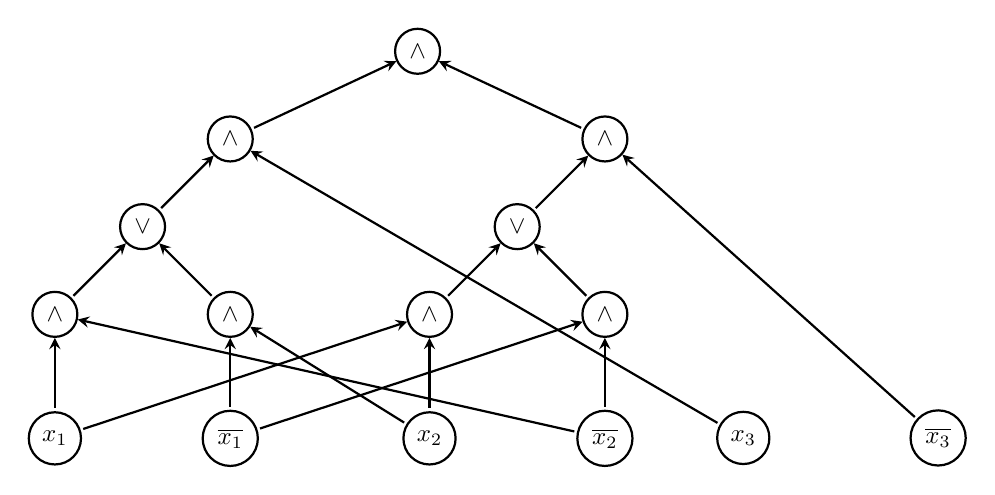
\begin{tikzpicture}[<-,>=stealth,shorten >=1pt,auto,node distance=1.75cm, thick,main node/.style={scale=0.9,circle,draw,font=\sffamily\normalsize}]

        \node[main node] (1) []{$\land$};

        \node[main node] (2) [below left of=1, xshift=-40]{$\land$};
        \node[main node] (3) [below right of=1, xshift=40]{$\land$};

        \node[main node] (4) [below left of=2]{$\lor$};
        \node[main node] (5) [below left of=4]{$\land$};
        \node[main node] (6) [below right of=4]{$\land$};
        \node[main node] (7) [below of=5]{$x_1$};
        \node[main node] (8) [below of=6]{$\overline{x_1}$};

        \node[main node] (9) [below left of=3]{$\lor$};
        \node[main node] (10) [below left of=9]{$\land$};
        \node[main node] (11) [below right of=9]{$\land$};

        \node[main node] (12) [below of=10]{$x_2$};
        \node[main node] (13) [below of=11]{$\overline{x_2}$};

        \node[] (14) [below right of=3, xshift=50]{};
        \node[] (15) [below left of=14]{};
        \node[] (16) [below right of=14]{};

        \node[main node] (17) [below of=15, yshift=8]{$x_3$};
        \node[main node] (18) [below of=16, yshift=8]{$\overline{x_3}$};

        \path[every node/.style={font=\sffamily\small}]
            (1) edge (2)
            (1) edge (3)

            (2) edge (4) 
            (2) edge (17)

            (3) edge (9)
            (3) edge (18)

            (4) edge (5)
            (4) edge (6)

            (5) edge (7)
            (5) edge (13)

            (6) edge (8)
            (6) edge (12)

            (10) edge (7)
            (10) edge (12)

            (11) edge (8)
            (11) edge (13)

            (9) edge (10)
            (9) edge (11)

            ;
    \end{tikzpicture}

    \caption{A Boolean circuit of size 15 and depth 4 computing $x_1 \oplus x_2 \oplus x_3$.}
\end{figure}

One of the most interesting properties of circuits is their strict relation to \textit{protocols}. Suppose that we have two parties, namely Alice and Bob, who want to cooperate in order to achieve a common objective, like computing a function. To reach their goal, Alice and Bob must carry out separate computations, communicating the result to the other party in a pre-defined sequence of steps. This idea serves as groundwork for a definition of protocols, algorithms that dictate such alternations between computation and communications. We give the following formal definition of protocol. \cite{comm_compl_appl}

\begin{definition}
 Let $X$ be Alice's input set and let $Y$ be Bob's input set. A protocol $\pi$ is a rooted directed binary tree whose leaves are associated with outputs and internal nodes are owned by either Alice or Bob, where the owner of $v$ is noted by $\mathrm{owner}(v)$. Each leaf is labeled with an output $o \in O$, where $O$ is the outcome set. Each internal node $v$ is also associated to a function $g_v : Z \to \{0,1\}$, where $Z = X$ if $\mathrm{owner}(v) = \mathrm{A}$ and $Z = Y$ if $\mathrm{owner}(v) = \mathrm{B}$.
\end{definition}

When given the input $(x,y) \in X \times Y$, the protocol computes the associated function of the current node (starting from the root), proceeding on the left child if the output is 0 and on the right child if the output is 1. When a leaf is reached, the protocol returns the associated output. The output of the protocol for a given input $(x,y)$ is denoted with $\pi(x,y)$. A function $f$ is said to be computed by the protocol $\pi$ if for all inputs $(x,y)$ it holds that $f(x,y) = \pi(x,y)$.

The complexity of protocols is measured in terms of their \textit{size} and \textit{depth}, that being the number of nodes of the protocol and the length of the longest directed path from the root node to a leaf. The \textbf{communication complexity} of a function $f$ is defined as the depth of the smallest protocol that computes $f$, corresponding to the minimal number of bits that must be communicated by Alice and Bob to compute $f$ for all possible inputs.

\begin{figure}[H]
    \centering

    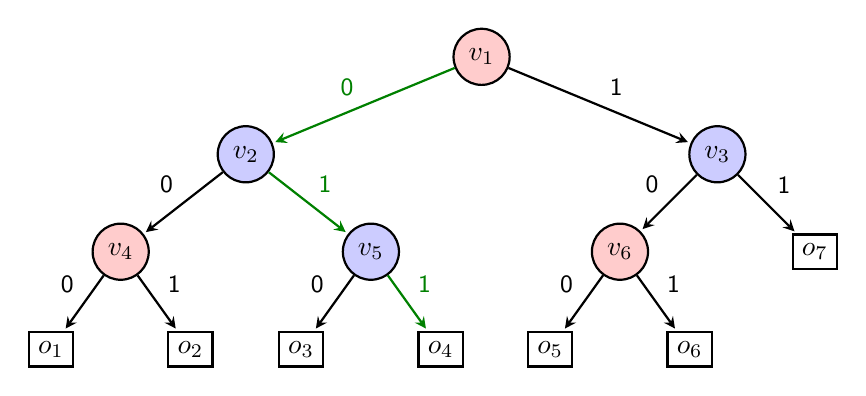
\begin{tikzpicture}[->,>=stealth,shorten >=1pt,auto,node distance=1.75cm, thick,main node/.style={scale=0.9,circle,draw,font=\sffamily\normalsize}]

        \node[circle, draw] (1)[fill=red!20] {$v_1$};

        \node[circle, draw] (2) [below left of=1, xshift=-50, fill=blue!20]{$v_2$};
        \node[circle, draw] (3) [below right of=1, xshift=50, fill=blue!20]{$v_3$};

        \node[circle, draw] (4) [below left of=2, xshift=-10, fill=red!20]{$v_4$};
        \node[circle, draw] (5) [below right of=2, xshift=10, fill=blue!20]{$v_5$};
        \node[circle, draw] (6) [below left of=3, fill=red!20]{$v_6$};
        \node[rectangle, draw] (7) [below right of=3]{$o_7$};

        \node[rectangle, draw] (8) [below left of=4, xshift=10]{$o_1$};
        \node[rectangle, draw] (9) [below right of=4, xshift=-10]{$o_2$};
        \node[rectangle, draw] (10) [below left of=5, xshift=10]{$o_3$};
        \node[rectangle, draw] (11) [below right of=5, xshift=-10]{$o_4$};
        \node[rectangle, draw] (12) [below left of=6, xshift=10]{$o_5$};
        \node[rectangle, draw] (13) [below right of=6, xshift=-10]{$o_6$};

        \path[every node/.style={font=\sffamily\small}]
            (1) edge[swap, color=Green]  node{0} (2)
            (1) edge node{1}(3)

            (2) edge[swap]  node{0} (4)
            (2) edge[color=Green]  node{1}(5)

            (3) edge[swap]  node{0} (6)
            (3) edge  node{1}(7)
                        
            (4) edge[swap]  node{0} (8)
            (4) edge  node{1}(9)

            (5) edge[swap]  node{0} (10)
            (5) edge[color=Green]  node{1}(11)

            (6) edge[swap]  node{0} (12)
            (6) edge  node{1}(13)
        ;
    \end{tikzpicture}

    \caption{An example of a protocol of size 13 and depth 3 where the red nodes are owned by Alice and the blue nodes are owned by Bob. The green path shows the computation given by $f_{v_1}(x) = 0$, $f_{v_2}(y) = 1$ and $f_{v_5}(y) = 1$ for the input $(x,y)$}
\end{figure}

A protocol encodes all possible messages that may be sent by the parties during any conceivable conversation, producing the expected output. This means that a protocol always returns an answer for all possible inputs, making any function computed by a protocol \textit{total}. This makes protocols are also a valid way to solve or verify total search problems.

In particular, for each \textsf{TFNP} problem $R$, we denote with $R^{cc}$ the equivalent $\mathsf{TFNP}^{cc}$ problem, where \textit{cc} stands for \textit{communication complexity}. Due to them being defined on two inputs instead of one, communication search problems are defined on two sets of input values instead of one.

\begin{definition}
 A communication search problem is a sequence $R = (R_n)_{n \in \N}$ of relations $R_n \subseteq \{0,1\}^n \times \{0,1\}^n \times O_n$, one for each $n \in \N$, where each $O_n$ is a finite set called \curlyquotes{outcome set}.
\end{definition}

A protocol is considered to be efficient when its communication complexity is polylogarithmic with respect to the bit-size of the inputs, i.e. equal to $O(\log^k n)$. This ensures that there is a Turing machine capable of simulating the protocol in polynomial time. We give the following definitions of $\mathsf{FP}^{cc}$ and $\mathsf{FNP}^{cc}$

\begin{definition}
 We define $\mathsf{FP}^{cc}$ as the set of communication search problems $R = (R_n)_{n \in \N}$ for which there exists a polylogarithmic depth protocol $\pi_n$ such that $\pi_n(x,y) = z$ if and only if $((x,y), z) \in R_n$. We define $\mathsf{FNP}^{cc}$ as the set of communication search problems $R = (R_n)_{n \in \N}$ for which there exists a polylogarithmic depth protocol $V_n$ such that $V_n((x,y), z) = 1$ if and only if $((x,y), z) \in R_n$. 
\end{definition}

In this case, the certificate is the protocol itself: it defines a schema through which a Turing machine can verify the solution. The concept of reduction also applies to communication search problems, but only under a pre-fixed value $t$ of the maximum amount of bits usable in the reduction, i.e. the maximum depth of the reduction protocol, which is necessary for computational reasons that we won't discuss. This allows us to define a $t$-bit \textsf{TFNP}$^{cc}$ hierarchy that follows the same structure as the standard one.

\newpage

\begin{definition}
    A communication search problem $R = (R_m)_{m \in \N}$, where $R_m \subseteq \{0,1\}^m \times \{0,1\}^m \times O_m$, is said to be many-to-one reducible into a search problem $S = (S_n)_{n \in \N}$, where $S_n \subseteq \{0,1\}^n \times \{0,1\}^n \times O_n'$, if for all $m \in \N$ there is an $n \in \N$ for which there are two functions $f_X, f_Y : \{0,1\}^m \to \{0,1\}^n$ and a $t$-bit protocol $g : (\{0,1\}^m \times \{0,1\}^n) \times O_n' \to O_m$ such that:
       \[\forall (x,y) \in \{0,1\}^m \times \{0,1\}^m \;\; (f_X(x), f_Y(y), z) \in S \implies (x, y, \pi((x,y), z)) \in R\]
    In other words, the functions $f_X,f_Y$ map inputs of $R$ into inputs of $S$, while the protocol $g$ maps solutions of $S$ into solutions of $R$. 
\end{definition}

Circuits and protocols are related one another through the \textbf{Karchmer-Widgerson game}. The game has a simple objective: given two inputs with different outputs, Alice and Bob have to cooperate to find a bit that differs between the two inputs. When the function is monotone, that being a function for which given any pair of inputs $x,y$ such that $x \leq y$ it also holds that $f(x) \leq f(y)$, the game is also called monotone. 

\begin{definition}
    Given a Boolean function $f : \{0, 1\}^n \to \{0, 1\}$, we define the Karchmer-Wigderson game of $f$, denoted with $\mathrm{KW}(f)$, as the following communication problem: given the two inputs $x$ and $y$, where $f(x) = 0$ and $f(y) = 1$, find an index $i \in [n]$ such that $x_i \neq y_i$.

    If $f$ is a monotone Boolean function, meaning that given two inputs $x,y$ if $x \leq y$ then $f(x) \leq f(y)$, the monotone Karchmer-Widgerson game of $f$, denoted with $\mathrm{mKW}(f)$, finds an index $i \in [n]$ such that $x_i < y_i$.
\end{definition}

These games were originally introduced in 1990 by Karchmer and Widgerson \cite{kw_games} to show how the communication complexity of a game for a function $f$ is equal to the circuit complexity of a \textit{Boolean circuit} that solves the game on $f$.

\begin{theorem}
    Given a function $f : \{0, 1\}^n \to \{0, 1\}$, there is a circuit of depth $d$ that computes $f$ if and only if there is a protocol of depth $d$ that solves $\mathrm{KW}(f)$. Moreover, if $f$ is monotone, the circuit is monotone and the protocol solves $\mathrm{mKW}(f)$
\end{theorem}

A surprising result \cite{span_programs, adventures_monotone_tfnp} proved that any communication search problem is equivalent to the monotone KW game of some Boolean function. This result implies that \textsf{TFNP}$^{cc}$ exactly is the study of the monotone Karchmer-Widgerson game.

\begin{lemma}
 For any communication search problem $R = (R_n)_{n \in \N}$, where $R_n \subseteq \{0,1\}^n \times \{0,1\}^n \times O_n$, in $t$-bit \textsf{TFNP}$^{cc}$, there is a function $f$ on $2^t\abs{O_n}$ variables such that $R$ is communication equivalent to $\mathrm{mKW}(f)$ under $t$-bit mapping reductions.
\end{lemma}

These results further extend the already known connections between search problems, communication complexity and circuit complexity, establishing that any result obtained in one of these models can be in some way established to the others.

\cleardoublepage


\chapter{Black-box TFNP} \label{chap:bb-tfnp}

\section{Oracles and decision trees}

In the previous chapter, we have briefly shown how \TFNP subclasses are defined in terms of basic existence principles that capture white-box total search problems solvable by protocols reducible to Karchmer-Widgerson games. From now on, we will shift our focus to the black-box model.

Black boxes have been used by complexity theorists since the early days, mostly through the concept of \textbf{oracle}, a device capable of instantly solving an instance of a designated problem. In particular, these problems may even be uncomputable, an assumption that allows us to view oracles as magical devices. Turing machines can be allowed to query such oracles to an additional \textit{oracle tape}. The machine writes a string on such tape, asking the oracle to solve the problem for that input. The output of the oracle is then written on the same tape, which can then be read by the Turing machine. Any query made to the oracle requires $\Theta(1)$ time, meaning that they don't influence the cost of the computation.

\begin{definition}
 An oracle for a problem $A$ is an external device that is capable of instantaneously solving an instance of $A$. An oracle Turing machine is a Turing machine provided with the ability to query an oracle. We write $M^A$ to describe a Turing machine provided with an oracle for the problem $A$.
\end{definition}

Given a class $\mathcal{C}$ and an oracle for a problem $A$, the \textit{relativized version} of the class $\mathcal{C}$, written $\mathcal{C}^A$ is the set of all problems of $\mathcal{C}$ solvable (or verifiable) with access to the oracle of $A$. For example, $\mathsf{P}^{\mathrm{SAT}}$ is the class of problems solvable in polynomial time by a Turing machine with an oracle for the $\mathrm{SAT}$ problem. More generally, given two classes $\mathcal{C}, \mathcal{B}$, we write $\mathcal{C}^{\mathcal{B}}$ to denote the set of all problems of $\mathcal{C}$ solvable (or verifiable) with access to an oracle for any problem that lies in $\mathcal{B}$. In other words, we have that $\mathcal{C}^{\mathcal{B}} = \bigcup_{A \in \mathcal{B}} \mathcal{C}^{A}$.

Oracles proved to be surprisingly useful for studying the relationship between $\mathsf{P}$ and $\mathsf{NP}$ by considering the relationship between $\mathsf{P}^A$ and $\mathsf{NP}^A$ for an oracle $A$. In a celebrated result \cite{relativization_p_np}, Baker et al. showed that there are two problems $A$ and $B$ such that $\mathsf{P}^A = \mathsf{NP}^A$ and $\mathsf{P}^B \neq \mathsf{NP}^B$. This fact makes many commonly used proof techniques useless against the conjecture, meaning that any answer to the $\mathsf{P} \stackrel{?}{=} \mathsf{NP}$ question will require techniques that are invariant with respect to the presence of an oracle.

Oracles provide a simple yet effective way to generalize the concept of reduction through the so-called \textit{Turing reductions}: if a Turing machine provided with an oracle for the problem $B$ is capable of resolving a problem $A$ then the problem $A$ can be reduced to solving multiple instances of the problem $B$. When $A$ is Turing reducible to $B$, we write $A \leq_T B$. Clearly, if the oracle machine $M^B$ can solve $A$ then any query to the oracle can be replaced with a call to a subroutine that solves $B$. This conversion is often referred to as \textit{de-relativization}. Many-to-one reductions can be seen as a specific case of Turing reductions, where the machine makes exactly one query to the oracle and then returns the output of such query.

In the particular case of total search problems, it was proven that the reducibility between search problems is strictly connected to the reducibility of their relativized versions up to all oracles \cite{rel_comp_np_search}.

\begin{theorem}
 Given two black-box search problems $R,S \in \mathsf{TFNP}$ and their relative classes it holds that $R \leq_m S$ if and only if $R^A \leq_m S^A$ for all oracles $A$.
\end{theorem}

This result implies that proving any relativized separation is equivalent to proving a non-relativized separation, allowing us to use the intuitive nature of oracles to rule out possible collapses in \TFNP subclasses. Many \TFNP subclasses have been proven to be different through separations between the respective query search problems. \cite{proofs_circuits_communication, tfnp_characterization}

\begin{definition}
 A query search problem is a sequence $R = (R_n)_{n \in \N}$ of relations $R_n \subseteq \{0,1\}^n \times O_n$, one for each $n \in \N$, where each $O_n$ is a finite set called \curlyquotes{outcome set}.
\end{definition}

A good eye will surely notice that the previous definition does not vary from the normal definition of search problems, unlike communication search problems. The only true difference resides in their computational models: query search problems are solved (or verified) through \textbf{decision trees}.

\begin{definition}[\cite{search_problems_dt_model}]
 A decision tree is a rooted directed binary tree whose nodes are associated with either an output value or an input Boolean variable. Each leaf is labeled with an output $o \in O$, where $O$ is the outcome set. Each internal node is labeled by a variable and the two outgoing edges are labeled by the two possible values of that variable.
\end{definition}

Decision trees can be viewed as nothing more than the black-box version of protocols: we don't care about who computes the next step or how they do it, we only care about the result being either a 0 or a 1 to proceed with the computation. In fact, like protocols, decision trees encode all possible ways to obtain a result, making them \textit{total}. Likewise, the complexity of a decision tree computing a function follows the same complexity measures as a protocol, i.e. its \textit{size} and its \textit{depth}. A function $f$ is said to be computed by the decision tree $T$ if for all inputs $x$ it holds that $f(x) = T(x)$. 

\begin{figure}[H]
    \centering

    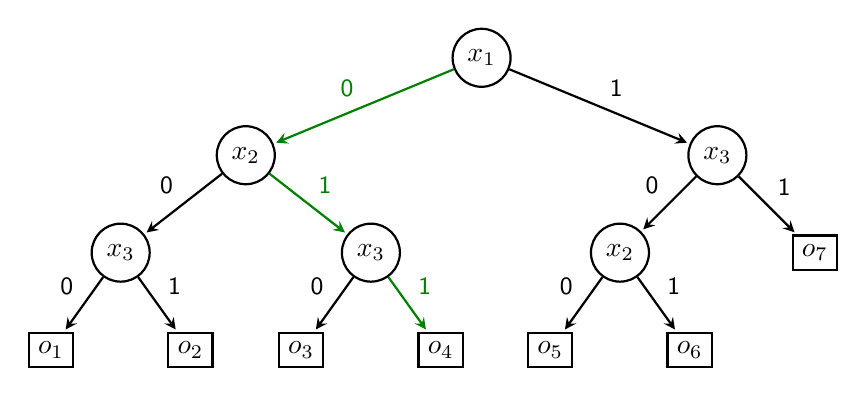
\begin{tikzpicture}[->,>=stealth,shorten >=1pt,auto,node distance=1.75cm, thick,main node/.style={scale=0.9,circle,draw,font=\sffamily\normalsize}]

        \node[circle, draw] (1)[] {$x_1$};

        \node[circle, draw] (2) [below left of=1, xshift=-50, ]{$x_2$};
        \node[circle, draw] (3) [below right of=1, xshift=50, ]{$x_3$};

        \node[circle, draw] (4) [below left of=2, xshift=-10, ]{$x_3$};
        \node[circle, draw] (5) [below right of=2, xshift=10, ]{$x_3$};
        \node[circle, draw] (6) [below left of=3, ]{$x_2$};
        \node[rectangle, draw] (7) [below right of=3]{$o_7$};

        \node[rectangle, draw] (8) [below left of=4, xshift=10]{$o_1$};
        \node[rectangle, draw] (9) [below right of=4, xshift=-10]{$o_2$};
        \node[rectangle, draw] (10) [below left of=5, xshift=10]{$o_3$};
        \node[rectangle, draw] (11) [below right of=5, xshift=-10]{$o_4$};
        \node[rectangle, draw] (12) [below left of=6, xshift=10]{$o_5$};
        \node[rectangle, draw] (13) [below right of=6, xshift=-10]{$o_6$};

        \path[every node/.style={font=\sffamily\small}]
 (1) edge[swap, color=Green]  node{0} (2)
 (1) edge node{1}(3)

 (2) edge[swap]  node{0} (4)
 (2) edge[color=Green]  node{1}(5)

 (3) edge[swap]  node{0} (6)
 (3) edge  node{1}(7)
            
 (4) edge[swap]  node{0} (8)
 (4) edge  node{1}(9)

 (5) edge[swap]  node{0} (10)
 (5) edge[color=Green]  node{1}(11)

 (6) edge[swap]  node{0} (12)
 (6) edge  node{1}(13)
 ;
    \end{tikzpicture}

    \caption{An example of a decision tree of size 13 and depth 3. The green path shows the computation made for the input $x = 011$.}
\end{figure}

Decision trees give an easier way to describe the computation of an oracle Turing machine: if $M^B$ solves (or verifies) a problem $A$ then the $i$-th query made by the procedure corresponds to a variable $x_i$ for the decision tree where $x_i = 1$ if the query returns a positive result and 0 otherwise. In other words, the computation tree of an oracle Turing machine can be viewed as a decision tree.

\begin{proposition}
 Given a search problem $A \in \mathsf{TFNP}$, if there is an oracle Turing machine $M^B$ that solves (or verifies) $A$ then there is a decision tree that solves (or verifies) $A$.
\end{proposition}

The above proposition gives a strong result that allows us to characterize black-box \TFNP through decision trees instead of oracles: \textit{any decision tree separation implies a relativized separation for some oracle} \cite{proofs_circuits_communication, tfnp_characterization}. As in the communication complexity formulation, given a \TFNP problem $R$, we denote with $R^{dt}$ the equivalent $\TFNP^{dt}$ problem, where \textit{dt} stands for \textit{decision tree}. We will omit this notation when the context makes it clear.

\begin{definition}
 We define $\mathsf{FP}^{dt}$ as the set of query search problems $R = (R_n)_{n \in \N}$ for which there exists a polylogarithmic depth decision tree $T_n$ such that $T_n(x) = y$ if and only if $(x,y) \in R_n$. Likewise, we define $\mathsf{FNP}^{dt}$ as the set of query search problems $R = (R_n)_{n \in \N}$ for which there exists a polylogarithmic depth decision tree family $\{T_y\}_{y \in \{0,1\}^m}$ such that $T_y(x) = 1$ if and only if $(x,y) \in R_n$.
\end{definition}

Like protocols, in query search problems the certificate is the verifying decision tree itself. Decision tree reductions are based on a more fine-grained definition, where the function that maps inputs of the first problem to inputs of the second problem is computed by many decision trees with output $\{0,1\}$.

\begin{definition}
 A query search problem $R = (R_m)_{m \in \N}$, where $R_m \subseteq \{0,1\}^m \times O_m$ is said to be many-to-one reducible to a query search problem $S = (S_n)_{n \in \N}$, where $S_n \subseteq \{0,1\}^n \times O_n'$, if for all $m \in \N$ there is an $n \in \N$ for which there is sequence $T = (T_i)_{i \in [n]}$ of decision trees $T_i : \{0,1\}^m \to \{0,1\}$ and a decision tree $T_y^o : \{0,1\}^m \to O_m$ for each $y \in O_n'$ such that:
    \[\forall x \in \{0,1\}^m \;\; (T(x), y) \in S \implies (x, T_y^o(x)) \in R\]
 where $T(x) := (T_1(x), \ldots, T_n(x))$.
\end{definition}

The difference in notation between $T_1, \ldots, T_n$ and $T_y^o$ underlines the fact that the former return a $\{0,1\}$ output, while the latter returns an output in $O_n$. The \textit{size} of the reduction is the number of input bits to $S$, that being $n$. The \textit{depth} $d$ of the reduction is the maximum depth of any tree involved in the reduction, meaning that
\[d = \max (\{\mathrm{depth}(T_i) : i \in [n]\} \cup \{\mathrm{depth}(T_y^o) : o \in O_m\})\]

The complexity of a reduction from $R$ to $S$, written as $S(R)$, is equal to the sum of the log of the size and the minimal depth of a decision tree reduction from $R$ to $S$, that is $S(R) = \log(m) + d$.

\begin{definition}
 Given $S \in \mathsf{TFNP}^{dt}$, we define the class $S^{dt}$ as the subset of \textsf{TFNP}$^{dt}$ problems efficiently reducible through decision trees to the problem $S$, formally $S^{dt} = \{R \in \mathsf{TFNP} \mid S(R) = O(\log^k n)\}$
\end{definition}

\section{Proof Complexity}

Like the white-box model, black-box total search problems can be studied under multiple lenses, such as \textbf{proof complexity}. This branch of complexity theory studies the complexity measures needed for a propositional formula to be proved by propositional proof systems, that being any system of rules that can prove the truthfulness of a propositional formula, i.e. a string made of logical operators applied on a set of $n$ variables, such as $F = x_1 \land (x_1 \to \lnot x_2 \lor x_3)$.

Any statement can be encoded by propositional formulas, which is either a \textit{tautology} (a statement that is always true), a \textit{satisfiable} formula (a statement that can be true or false based on the assignment) or an \textit{unsatisfiable} formula (a statement that is always false). Proving that a formula $F$ is a tautology is equivalent to proving that $\lnot F$ is unsatisfiable.

Proof systems can be viewed as an algorithm that manipulates propositional formulas, producing a new formula. When a formula $G$ is derived by the formula $F$ in the proof system $S$, we write $F \stackrel{S}{\vdash} G$. Proof systems must be \textit{sound}: if $F \stackrel{S}{\vdash} G$ then $G$ is a \textit{logical consequence} of $F$, which means that $F \to G$ is a tautology. In 1979, Cook and Reckhow gave the following formal definition of propositional proof system - often called Cook-Reckhow proof systems.

\begin{definition}
 A propositional proof system (or pps) is a polynomial time computable surjective function $f : \Sigma^* \to \mathrm{TAUT}$, where $\mathrm{TAUT}$ is the set of logical tautologies.
\end{definition}

Given a formula $F \in \mathrm{TAUT}$ a string $s \in \Sigma^*$ and a proof system $f$, we say that $s$ encodes $F$ for the pps $f$ if it holds that $f(s) = F$. This idea justifies why we want proof systems to be surjective: any true statement must have a valid encoding in the proof system. This property is called \textit{completeness} of the proof system.

The most studied proof system is \textbf{Resolution} (or \textsf{Res}). Given a formula $F \in \mathrm{TAUT}$, this proof system can prove that it is a tautology by proving that $\lnot F \in \mathrm{UNSAT}$.

A \textit{conjunctive normal form} (CNF) formula $F$ is a conjunction of $m$ \textit{clauses} $C_1, \ldots, C_m$, where $C_i$ is a disjunction of $k_i$ \textit{literals}, that being either a variable defined on $F$ or its negation. For example, the following formula is in conjunctive normal $F = (x_1 \lor x_2 \lor \lnot{x_3} \lor x_4) \land (x_1 \lor \lnot{x_2}) \land x_3$

Any formula can be expressed as an equivalent CNF formula, making Resolution a \textit{complete} and \textit{sound} proof system. Resolution proofs are based on repeated applications of the following simple rule called the \textit{resolution rule}:
\[\dfrac{C \lor x \qquad D \lor \lnot x}{C \lor D}\]

Given a CNF formula $F = C_1 \land \ldots \land C_m$ and a clause $C$, we have that $F \stackrel{\mathsf{Res}}{\vdash} C$ if there is a sequence of clauses $D_1, \ldots, D_k$ such that $D_k = C$ and each $D_i$ in the sequence is either an \textit{axiom} of $F$ (meaning that $D_i = C_j$ for some $j$) or is obtained by applying the resolution rule on $D_p$ and $D_q$ for some $p,q < i$. Resolution is able to prove that a CNF formula $\lnot F$ is unsatisfiable by deriving the empty clause $\bot$ starting from the axioms of the formula itself. A Resolution proof is often referred to as a \textit{refutation}.

For example, given the following unsatisfiable CNF formula $(y \lor z) \land (y \lor \overline{z}) \land (x \lor \overline{y} \lor z) \land (\overline{x} \lor \overline{y} \lor z) \land \overline{z}$, a Resolution proof is given by:
\[\begin{array}{lcl}
    D_1 :& \overline{z} & \text{Axiom} \\
    D_2 :& \overline{x} \lor \overline{y} \lor z & \text{Axiom} \\
    D_3 :& x \lor \overline{y} \lor z & \text{Axiom} \\
    D_4 :& \overline{x} \lor \overline{y} & \text{Res. on $D_1, D_2$} \\
    D_5 :& x \lor \overline{y} & \text{Res. on $D_1, D_3$} \\
    D_6 :& y \lor z & \text{Axiom} \\
    D_7 :& y \lor \overline{z} & \text{Axiom} \\
    D_8 :& y & \text{Res. on $D_6,D_7$} \\
    D_9 :& \overline{x} & \text{Res. on $D_4, D_8$} \\
    D_{10} :& x & \text{Res. on $D_5, D_8$} \\
    D_{11} :& \bot & \text{Res. on $D_9, D_10$} \\
\end{array}\]
\noindent

The \textit{length} of a resolution refutation is the number of clauses in the refutation, while the \textit{width} is the maximum number of literals that can be found in any of its clauses. For instance, the previous refutation has length 11 and width 3.

To make things easier to read, each refutation can also be graphically represented by connecting clauses with lines. Resolution refutations expressed in this form are also called DAG-like refutations.

\begin{figure}[H]
    \centering
    
        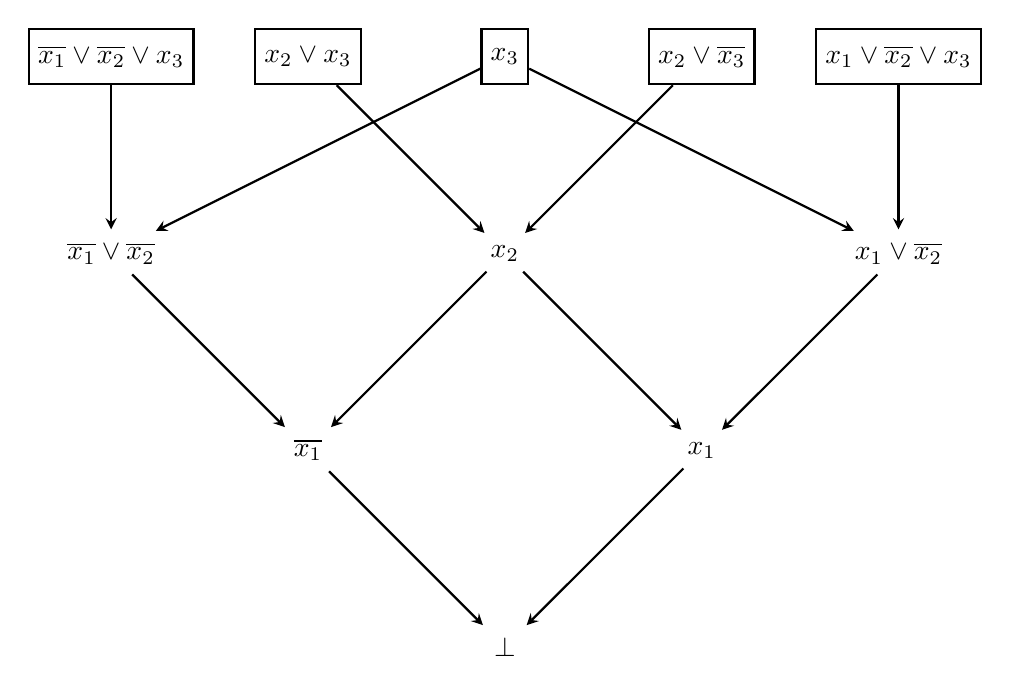
\begin{tikzpicture}[->,>=stealth,shorten >=1pt,auto,node distance=2.5cm, thick,main node/.style={scale=0.9,circle,draw,font=\sffamily\normalsize}]
            \node [rectangle, draw, minimum height=20](1) []{$\overline{x_1} \lor \overline{x_2} \lor x_3$};
            \node [rectangle, draw, minimum height=20](2) [right of=1]{$x_2 \lor x_3$};
            \node [rectangle, draw, minimum height=20](3) [right of=2]{$x_3$};
            \node [rectangle, draw, minimum height=20](4) [right of=3]{$x_2 \lor \overline{x_3}$};
            \node [rectangle, draw, minimum height=20](5) [right of=4]{$x_1 \lor \overline{x_2} \lor x_3$};

            \node (6) [below of=1]{$\overline{x_1} \lor \overline{x_2}$};
            \node (x) [below of=2]{};
            \node (7) [below of=3]{$x_2$};
            \node (y) [below of=4]{};
            \node (8) [below of=5]{$x_1 \lor \overline{x_2}$};

            \node (9) [below of=x]{$\overline{x_1}$};
            \node (10) [below of=y]{$x_1$};
            \node (z) [below of=7]{};
            
            \node (11) [below of=z]{$\bot$};
        
            \path[every node/.style={font=\sffamily\small}]
                (1) edge (6)
                (2) edge (7)
                (3) edge (6)
                (3) edge (8)
                (4) edge (7)
                (5) edge (8)

                (6) edge (9)
                (7) edge (9)
                (7) edge (10)
                (8) edge (10)

                (9) edge (11)
                (10) edge (11)
                ;
        \end{tikzpicture}
    
    \caption{Dag-like refutation of the previous formula.}
\end{figure}

By definition, each clause $D_i$ can be used as premise for more than one rule application, both through weakening and resolution. When each $D_i$ of the proof is used \textbf{only once}, we say that it is a \textbf{tree-like refutation} due to how the underlying DAG becomes a tree. This restriction implies that if we want to use a clause multiple times then it must be derived again (or simply copied if it's an axiom). Clearly, this duplication process allows us to transform any dag-like refutation into a tree-like refutation, but this usually blows up the length of the proof exponentially.

\begin{figure}[H]
    \centering
    
    \resizebox{1\hsize}{!}{
        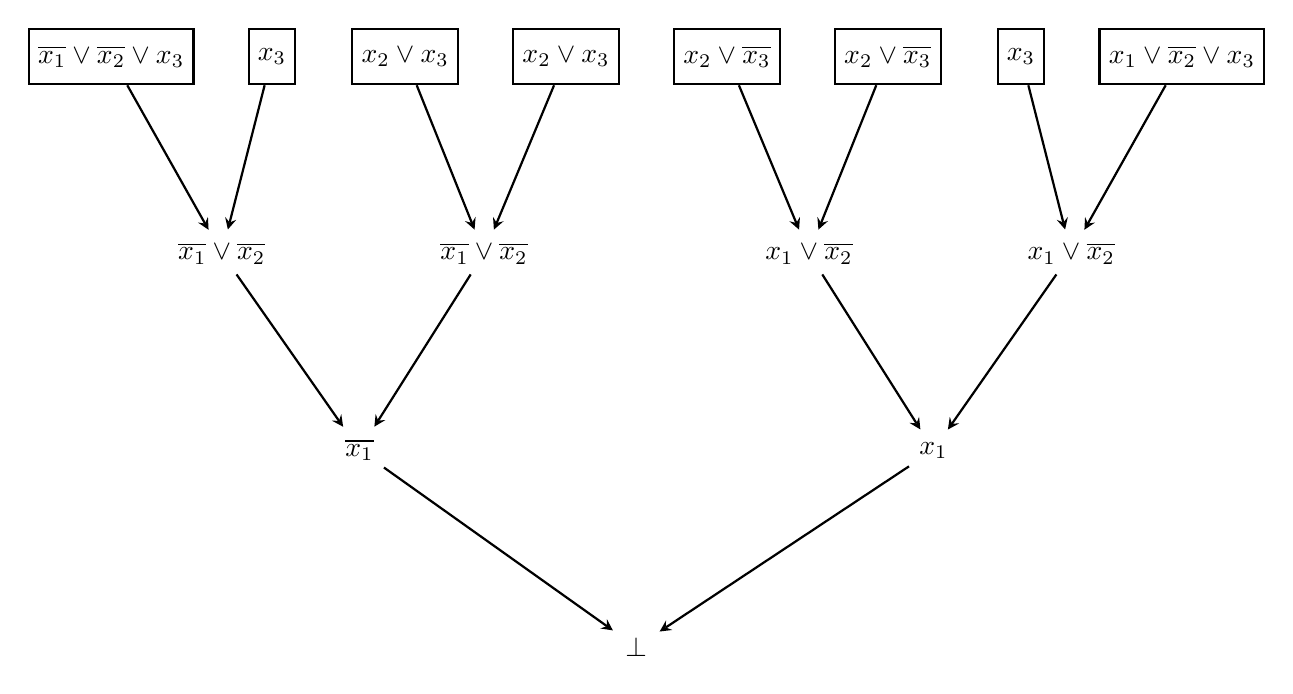
\begin{tikzpicture}[->,>=stealth,shorten >=1pt,auto,node distance=2.5cm, thick,main node/.style={scale=0.9,circle,draw,font=\sffamily\normalsize}]
            \node [rectangle, draw, minimum height=20](1) []{$\overline{x_1} \lor \overline{x_2} \lor x_3$};
            \node [rectangle, draw, minimum height=20](2) [right of=1, xshift=-13]{$x_3$};
            \node [rectangle, draw, minimum height=20](3) [right of=2, xshift=-23]{$x_2 \lor x_3$};
            \node [rectangle, draw, minimum height=20](4) [right of=3, xshift=-13]{$x_2 \lor x_3$};
            \node [rectangle, draw, minimum height=20](5) [right of=4, xshift=-13]{$x_2 \lor \overline{x_3}$};
            \node [rectangle, draw, minimum height=20](6) [right of=5, xshift=-13]{$x_2 \lor \overline{x_3}$};
            \node [rectangle, draw, minimum height=20](7) [right of=6, xshift=-23]{$x_3$};
            \node [rectangle, draw, minimum height=20](8) [right of=7, xshift=-13]{$x_1 \lor \overline{x_2} \lor x_3$}; 

            \node (9)[below of=1, xshift=40]{$\overline{x_1} \lor \overline{x_2}$};
            \node (10)[below of=3, xshift=28.5]{$\overline{x_1} \lor \overline{x_2}$};
            \node (11)[below of=6, xshift=-28.5]{$x_1 \lor \overline{x_2}$};
            \node (12)[below of=8, xshift=-40]{$x_1 \lor \overline{x_2}$};

            \node (13)[below of=10, xshift=-45]{$\overline{x_1}$};
            \node (14)[below of=11, xshift=45]{$x_1$};

            \node (15)[below of=13, xshift=100]{$\bot$};
        
            \path[every node/.style={font=\sffamily\small}]
                (1) edge (9)
                (2) edge (9)
                (3) edge (10)
                (4) edge (10)
                (5) edge (11)
                (6) edge (11)
                (7) edge (12)
                (8) edge (12)

                (9) edge (13)
                (10) edge (13)
                (11) edge (14)
                (12) edge (14)

                (13) edge (15)
                (14) edge (15)
                ;
        \end{tikzpicture}
    }
    
    \caption{Tree-like refutation of the previous formula.}
    \label{treelike_res_proof}
\end{figure}

This subset of proofs defines a more specific proof system called \textit{Tree-like Resolution} (or \textsf{TreeRes}). Generally, this type of refutation produces a proof of exponential length compared to the number of variables defined on the formula itself. Resolution and Tree-like Resolution are separated, meaning that some proofs are easy for the former and hard for the latter, making Resolution a stronger proof system.

Resolution has three main complexity measures: size, depth and width. The \textit{size} of a Resolution proof is the total number of nodes appearing in the proof. The \textit{depth} of a Tree-like Resolution proof is the length of the longest path from an axiom to the empty clause. For example, the proof shown in \Cref{treelike_res_proof} has size 9, depth 3 and width 3. These three complexity measures are highly related. For example, if a Tree-like Resolution proof has depth $d$ the size of such proof is $O(2^{d+1})$ since a $d$-depth tree can have at most $2^{d+1}-1$ nodes.

But why are we interested in proving or refusing propositional formulas? We discussed how the $\mathrm{SAT}$ problem is \textsf{NP}-Complete. This clearly implies that the problem $\overline{SAT}$ is \textsf{coNP}-Complete. This fact can be used to show that $\overline{SAT} \leq_m \mathrm{UNSAT} \leq_m \mathrm{TAUT}$, implying that both $\mathrm{UNSAT}$ and $\mathrm{TAUT}$ are also \textsf{coNP}-Complete. Showing that any of these problems is also in $\mathsf{NP}$ would answer the $\mathsf{NP} \stackrel{?}{=} \mathsf{coNP}$ question.

Proof systems are essential to work on this question: given the encoding $\Pi$ of a proof of $F$ in a proof system, a verifier can follow the rules defined by the proof system to prove that $F$ is indeed a tautology. In this case, $\Pi$ serves as a certificate for $F$ while the pps defines the verifier. We give the following equivalent definition of a propositional proof system.

\begin{definition}
 A propositional proof system (or pps) is a verifier $V$ such that $F \in \mathrm{TAUT}$ if and only if there is a string $\Pi \in \Sigma^*$ such that $V(F,\Pi) = 1$ and that runs in polynomial time with respect to $\abs{F} + \abs{\Pi}$. 
\end{definition}

At first glance, one could think that this definition implies that any complete and sound pps proves that $\mathrm{TAUT} \in \mathsf{NP}$. However, we must also consider the length of such proofs: to be an efficient verifier, the length of the certificates must be polynomially bounded by the length of $F$. In other words, it must hold that $\abs{\Pi} = O(\abs{F}^k)$ for some $k \in \N$. This means that in order to prove that $\mathsf{NP} \neq \mathsf{coNP}$, or equivalently that $\mathrm{TAUT} \in \mathsf{NP}$, we must find a \textbf{polynomially bounded proof system}, a pps that uses only polynomially bounded proofs for all tautologies.

\begin{proposition}
 There is a polynomially bounded proof system if and only if $\mathsf{NP} = \mathsf{coNP}$.
\end{proposition}

We already discussed how researchers believe that $\mathsf{NP} \neq \mathsf{coNP}$ is the expected answer to the conjecture. Proving this statement is no easy task: we would have to prove that there is a particular formula $F$ that strictly requires an exponential length encoding for every discovered and undiscovered proof system.

\newpage

\section{The Black-box model and Proof complexity}

Proof complexity is highly related to other branches of complexity theory, including the study of total search problems. In order to get to this relation between proof complexity and $\mathsf{TFNP}^{dt}$, we have to restrict our focus to CNF formulas. By construction, a CNF formula can be unsatisfiable if and only if for all assignments $\alpha(x_1, \ldots, x_n)$ there is a clause $C_i$ that is false. It's easy to see this fact implies that any CNF formula gives rise to an associated search problem: finding a falsified clause inside the formula (if there is any) for each possible assignment.

\begin{definition}
 Given a CNF $F = C_1 \land \ldots \land C_m$ over $n$ variables, we define $\mathrm{Search}(F)$ as the following search problem: given an input assignment $\alpha(x_1, \ldots, x_n)$, return an index $i$ such that the assignment falsifies $C_i$.
\end{definition}

This problem is usually referred to as the \textbf{false clause search problem}. When $F$ is an unsatisfiable CNF formula, $\mathrm{Search}(F)$ is a total search problem since for any input assignment there will always be an unsatisfied clause. Moreover, the search problem of any unsatisfiable formula can easily be solved (or verified) by a decision tree for any formula $F$: if the assignment $\alpha(x_1 = b_1, \ldots, x_n = b_2)$ falsifies the clause $C_i$, define a path $x_1 = b_1, \ldots, x_n = b_n$ on the decision tree and let $C_i$ be the output of such path. In other words, for all $\lnot F \in \mathrm{TAUT}$ it holds that $\mathrm{Search}(F) \in \mathsf{TFNP}^{dt}$. 

\begin{figure}[H]
    \centering
    
    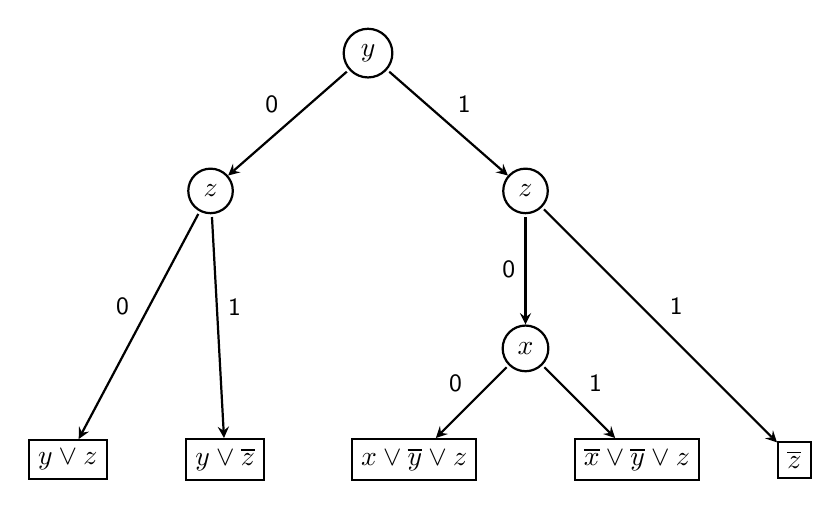
\begin{tikzpicture}[<-,>=stealth,shorten >=1pt,auto,node distance=2cm, thick,main node/.style={scale=0.9,circle,draw,font=\sffamily\normalsize}]
    
        \node (1)[circle, draw]{$y$};
        
        \node (2) at ($(1)+(-2,-1.75)$) [circle, draw]{$z$};
        \node (3) at ($(1)+(2,-1.75)$) [circle, draw]{$z$};
    
        \node (4) [below left of=2]{};
        \node (5) [below right of=2]{};
    
        \node (6) [below of=3, circle, draw]{$x$};
        
        \node (8) [below left of=6, rectangle, draw]{$x \lor \lnot{y} \lor z$};
        \node (9) [below right of=6, rectangle, draw]{$\lnot{x} \lor \lnot y \lor z$};
    
        \node (11) [right of=9, rectangle, draw]{$\lnot{z}$};
    
        \node (14) at ($(8)+(-2.4,0)$) [rectangle, draw]{$y \lor \lnot{z}$};
        \node (15) [left of=14, rectangle, draw]{$y \lor z$};
    
        \path[every node/.style={font=\sffamily\small}]
 (14) edge [swap] node{1} (2)
 (15) edge node{0} (2)
    
 (8) edge node{0}(6)
 (9) edge node[swap]{1}(6)
    
 (6) edge node{0}(3)
 (11) edge [swap] node{1}(3)
    
 (2) edge node {0} (1)
 (3) edge node [swap] {1} (1)
 ;
    \end{tikzpicture}
    
    \caption{Decision tree for the previous unsatisfiable formula.}
    \end{figure}

Similarly, we can show that any total query search problem $R$ can be associated with the search problem of the formula $F$ that describes the set of decision trees that verify $R$. Consider a decision tree $T$ made of the paths $p_1, \ldots, p_k$, each leading to the leaves $\ell_1, \ldots, \ell_k$. The DNF encoding of $T$, written as $D(T)$, is the disjunction over the conjunction of the literals $\alpha_1, \ldots, \alpha_h$ along each of the accepting paths in $T$. In other words, we have that $D_T = p_1 \lor \ldots \lor p_k$ where each $p_i = \alpha_1 \land \ldots \land \alpha_h \land \ell_i$ is an accepting path of $T$. By De Morgan's theorem, $\lnot{D(T)}$ is a CNF.

\begin{proposition}
    \label{Rdt = Search(F)}
 Given a total query search problem $R \subseteq \{0,1\}^n \times O$, for each $n \in \N$ there exists an unsatisfiable CNF formula $F_n$ defined over $\abs{O}$-many variables such that $R_n = \mathrm{Search}(F_n)$. This formula is called canonical CNF encoding of $R_n$.
\end{proposition}

\begin{proof}
 Since $R = (R_n)_{n \in \N} \in \TFNP^{dt}$, for each $y \in O_n$ there is a $\mathrm{polylog}(n)$-depth decision tree $T_y$ that verifies $R_n$. Consider the CNF $F_n := \bigwedge\limits_{y \in O_n} \lnot{D(T_y)}$. Since $R$ is a total search problem, for each input $x$ there is a valid output, implying that at least one tree $T_y$ will have an accepting path, meaning that $D(T_y)$ with input $x$ accepts and therefore $\lnot{D(T_y)}$ with input $x$ rejects, concluding that $F_n$ is unsatisfiable. Moreover, this formulation also concludes that:
    \[(x,y) \in R_n \iff (x,y) \in \mathrm{Search}(F_n)\]
 and thus that $R_n = \mathrm{Search}(F_n)$.

\end{proof}

This result clearly implies that $(R)_{n \in \N} = (\mathrm{Search}(F_n))_{n \in \N}$, where $F_1, F_2, \ldots$ is a family of CNF formulas, and by extension that black-box \TFNP is exactly the study of the false clause search problem. Like in the communication \TFNP case, the upshot is that it is sufficient to restrict our interests to the study of search problems associated with unsatisfiable CNF formulas.

Furthermore, we also notice that the width of each CNF encoding of a given search problem in \textsf{TFNP}$^{dt}$ corresponds to the maximum depth of the decision trees that solve or verify it.

Through this connection, Göös et al. \cite{adventures_monotone_tfnp} showed that many important proof systems are characterized by an associated $\mathsf{TFNP}^{dt}$ search problem and vice versa. Given a proof system $P$ and an unsatisfiable CNF formula $F$, the \textbf{complexity} required by $P$ to prove $F$ is given by:
\[P(F) := \min\{\log \mathrm{size}(\Pi) + \mathrm{deg}(\Pi) : \Pi \text{ is a $P$-proof of } F\}\]
where $\mathrm{size}(\Pi)$ is the the total number of symbols in $\Pi$ and $\mathrm{deg}(\Pi)$ is the \textit{degree} of $\Pi$ associated to $P$, which varies from proof system to proof system. For example, in Tree-like Resolution the degree is the \textit{depth} of the proof, while in Resolution the degree is the \textit{width} of the proof. This degree measure will be specified for the proof systems analyzed in the following sections.

To make things more readable, we will refer to $\mathrm{Search}(F)$ as $S_F$. Since each $\TFNPdt$ problem is equivalent to $S_F$ for some formula $F$, the complexity parameter defined above can be used to give another \textbf{characterization} of $\TFNPdt$ problems.

\begin{definition}
 We say that a proof system $P$ characterizes a $\TFNPdt$ problem $R$ (and reflexively that $R$ characterizes $P$) if it holds that \[R^{dt} = \{S_F : P(F) = \mathrm{polylog}(n)\}\]
 where $F = (F_i)_{i \in \N}$ is a family of formulas. In a stronger sense, it must hold that $R^{dt}(S_F) = \Theta(P(F))$. 
\end{definition}

Again, this implies that the encoding CNF formulas must have a polylogarithmic width. Most of the \TFNP subclasses discussed in previous sections have been shown to have a characterizing proof system:
\begin{itemize}
    \item $\mathrm{FP}^{dt}(S_F) = \Theta(\mathsf{TreeRes}(F))$ \cite{search_problems_dt_model}
    \item $\mathrm{PLS}^{dt}(S_F) = \Theta(\mathsf{Res}(F))$  \cite{approx_counting}
    \item $\mathrm{PPA}^{dt}(S_F) = \Theta(\F_2\textsf{-NS}(F))$ \cite{adventures_monotone_tfnp}
    \item $\mathrm{PPADS}^{dt}(S_F) = \Theta(\textsf{unary-NS}(F))$ \cite{separations_proof_complexity}
    \item $\mathrm{PPAD}^{dt}(S_F) = \Theta(\textsf{unary-SA}(F))$ \cite{separations_proof_complexity}
    \item $\mathrm{SOPL}^{dt}(S_F) = \Theta(\mathsf{RevRes}(F))$ \cite{separations_proof_complexity}
    \item $\mathrm{CLS}^{dt}(S_F) = \Theta(\mathsf{RevResT}(F))$ \cite{separations_proof_complexity}
\end{itemize}

\begin{figure}[H]
    \centering
    
    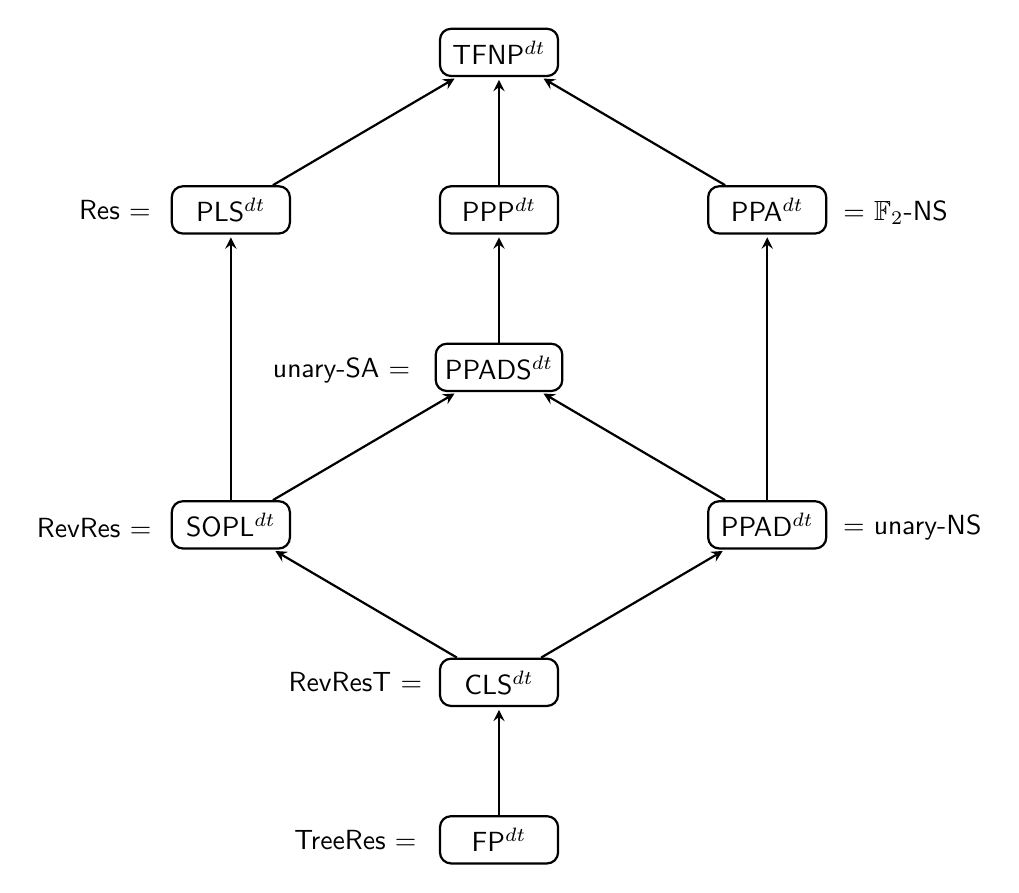
\begin{tikzpicture}[->,>=stealth,shorten >=1pt,auto,node distance=2cm, thick,main node/.style={scale=0.9,circle,draw,font=\sffamily\normalsize}]
    
        \node[rectangle, draw, rounded corners, minimum width=15mm, minimum height=6mm] (2) []{\textsf{TFNP}$^{dt}$};

        \node[rectangle, draw, rounded corners, minimum width=15mm, minimum height=6mm] (3) [below of = 2]{\textsf{PPP}$^{dt}$};

        \node[rectangle, draw, rounded corners, minimum width=15mm, minimum height=6mm] (4) [left of = 3, xshift=-40]{\textsf{PLS}$^{dt}$};

        \node[rectangle, draw, rounded corners, minimum width=15mm, minimum height=6mm] (5) [right of = 3, xshift=40]{\textsf{PPA}$^{dt}$};

        \node[rectangle, draw, rounded corners, minimum width=15mm, minimum height=6mm] (6) [below of = 3]{\textsf{PPADS}$^{dt}$};

        \node (7) [below of = 6]{};

        \node[rectangle, draw, rounded corners, minimum width=15mm, minimum height=6mm] (8) [left of = 7, xshift=-40]{\textsf{SOPL}$^{dt}$};

        \node[rectangle, draw, rounded corners, minimum width=15mm, minimum height=6mm] (9) [right of = 7, xshift=40]{\textsf{PPAD}$^{dt}$};

        \node[rectangle, draw, rounded corners, minimum width=15mm, minimum height=6mm] (10) [below of = 7]{\textsf{CLS}$^{dt}$};

        \node[rectangle, draw, rounded corners, minimum width=15mm, minimum height=6mm] (11) [below of = 10]{\textsf{FP}$^{dt}$};

        \node (12) [left of = 4, xshift = 15]{\textsf{Res} $=$};

        \node (13) [left of = 6, yshift = -1]{\textsf{unary-SA} $=$};
        
        \node (14) [left of = 8, xshift = 7.5, yshift = -1]{\textsf{RevRes} $=$};
        
        \node (15) [left of = 10, xshift = 5]{\textsf{RevResT} $=$};

        \node (16) [right of = 5, xshift = -10.5, yshift = -1]{$=$ \textsf{$\F_2$-NS}};

        \node (17) [right of = 9, xshift = -4.5, yshift = -1]{$=$ \textsf{unary-NS}};

        \node (18) [left of = 11, xshift = 5]{\textsf{TreeRes} $=$};
    
        \path[every node/.style={font=\sffamily\small}]
 (3) edge (2)
 (4) edge (2)
 (5) edge (2)
 (6) edge (3)
 (8) edge (4)
 (8) edge (6)
 (9) edge (5)
 (9) edge (6)
 (10) edge (8)
 (10) edge (9)
 (11) edge (10)
 ;
    \end{tikzpicture}
    
    \caption{Black-box \textsf{TFNP} classes and their characterizing proof systems.}
    \label{TFNP_dt_hierarchy}
\end{figure}

\quad

\section{Reductions through CNF formulas}

Intuitively, the characterization given in the previous section shows that any $\TFNPdt$ problem can be transformed into a proof system for refuting unsatisfiable CNF formulas of polylogarithmic width: since any $\TFNPdt$ is equivalent to the search problem for some unsatisfiable CNF formula, any efficient decision tree reduction between problems is nothing more than an efficient proof in the characterizing proof system and vice versa. To formalize this idea, we introduce the concept of \textbf{reductions between CNF formulas} \cite{tfnp_characterization}.

Suppose that $C$ is a clause over $n$ variables and that $T = (T_i)_{i \in [n]}$ is a sequence of depth-$d$ decision trees, where $T_i : \{0,1\}^{m} \to \{0,1\}$. We refer to $C(T)$ as the CNF formula obtained by substituting each variable $x_i$ in $C$ with $D(T_i)$ and rewriting the result as a CNF, or more conveniently:
\[C(T) := \bigwedge_{i \in [n]} \, \bigwedge_{\substack{r \,:\, \text{rejecting} \\ \text{path of $T_i$}}} \lnot{r}\]

\begin{definition}
 Let $F = C_1 \land \ldots \land C_{m_F}$ be an unsatisfiable CNF over $n_F$ variables. We say that a CNF formula $H$ made of $m_H$ clauses over $n_H$ variables reduces to $F$ via depth-$d$ decision trees if there exist two sequences of depth-$d$ decision trees $T = (T_i)_{i \in [n_F]}$ and $T^o = (T_j^o)_{j \in [m_F]}$, where $T_i : \{0,1\}^{n_H} \to \{0,1\}$ and $T_j^o : \{0,1\}^{n_H} \to [m_H]$, such that given the following formula:
    \[F_H := \bigwedge_{j \in [m_F]} \,\bigwedge_{\substack{p \,:\; \text{path} \\ \text{in } T_j^o}} C_i(T) \lor \lnot{p}\]
 it holds that if $F$ is unsatisfiable then $F_H$ is unsatisfiable and by consequence that $H$ is unsatisfiable. 
\end{definition}

In particular, we notice that $F_H$ can also be written as a CNF by simply distributing each $\lnot{p}$ inside $C_i(T)$. Each clause $C_i(T) \lor \lnot{p}$ must be either tautological (since it could contain a variable and its negation) or a weakening of the corresponding clause of $H$ - meaning that it is a formula $Q$ such that $H \to Q$ - indexed by the label at the end of the path $p$. Moreover, we notice that through this formulation any depth-$d$ decision tree reduction from $S_H$ to $S_F$ induces the search problem $S_{F_H}$. By construction, reductions between CNF formulas are just a formal way to say that reductions between search problems reduction are actually proof systems.

\begin{definition}
 Given a problem $S_F \in \TFNPdt$ the \textbf{canonical proof system} of such problem, written as $P_F$, is a proof system that refutes an unsatisfiable formula $H$ over $n_H$ variables if $H$ is reducible to an instance of $F$ over $n_F$ variables. 
\end{definition} 

A $P_F$-proof of $H$ consists of the decision trees that make such reduction possible. The \textit{size} of such proof is given by $n_F$, while the \textit{degree} is given by the maximum depth among the involved decision trees. Hence, the $P_F$ complexity of $H$ is given by:
    \[P_F(H) := \min\{\log \mathrm{size(\Pi)}+ \mathrm{depth}(\Pi) : \Pi \text{ is a $P_F$-proof of } H\}\]

This definition directly implies that given $S_F \in \TFNPdt$, the \textbf{characterizing proof system} of $S_F^{dt}$ is equivalent to the canonical proof system $P_F$. Canonical proof systems are \textit{sound}, since by construction any valid substitution of an unsatisfiable CNF formula is also unsatisfiable, and also \textit{efficiently verifiable}, since it suffices to check that each of the clauses of $F_H$ is either tautological or a weakening of a clause in $H$, which can both be done in polynomial time compared to the size of the proof.

The following theorem plays a crucial role in $\TFNPdt$ characterization through proof complexity, stating that the proof system $P_F$ has a short proof of $H$ if and only if $S_H$ efficiently reduces to $S_F$. In other words, an efficient proof of a formula in a characterizing proof system automatically gives an efficient reduction to the corresponding complete search problem.

\newpage

\begin{theorem}
    \label{equiv_proof}
 Let $S_F \in \TFNPdt$ and let $H$ be an unsatisfiable CNF formula. The two following results hold:
    \begin{enumerate}
        \item If $H$ has a size $s$ and depth $d$ proof in $P_F$ then $S_H$ has a size $O(s)$ and depth $d$ reduction to $S_F$
        \item If $S_H$ has a size $s$ and depth $d$ decision tree reduction to $S_F$ then $H$ has a size $s2^{O(d)}$ and depth $d$ proof in $P_F$
    \end{enumerate}
 In particular, this implies that $S_F^{dt}(S_H) = \Theta(P_F(H))$.
\end{theorem}


\begin{proof}
 Suppose that $T = (T_i)_{i \in [n_F]}$ and $T' = (T_j^o)_{j \in [m_F]}$ is a $P_F$ proof of $H$ of size $s$ and depth $d$. Given any assignment $\alpha$ such that $(\alpha, i) \in S_F$, let $C_i$ be the clause of $F$ falsified by $T_1(\alpha), \ldots, T_{n_F}(\alpha)$ and let $p$ be the path followed by $T_i^o(\alpha)$. It's easy to see that a clause of the formula $C_i(T) \lor \lnot{p}$ must be falsified by $\alpha$. In particular, such clause is also the weakening of the $T_i^o(\alpha)$-th clause of $H$, concluding that $(\alpha, T_i^o(\alpha)) \in S_H$. In other words, the $P_F$ proof of $H$ corresponds to a reduction from $S_H$ to $S_F$ of size $n_F = O(s)$ and depth $d$.

 Vice versa, suppose that $T = (T_i)_{i \in [n_F]}$ and $T' = (T_j^o)_{j \in [m_F]}$ is a decision tree reduction from $S_H$ to $S_F$ of size $s$ and depth $d$. Then, we can construct $F_H$ as previously described through the use of these decision trees. Let $L$ be a clause of $C_i(T)$ for some $i \in [m_F]$ and let $p$ be any path in $T_i^o$. If the formula $C_i(T) \lor \lnot{p}$ is tautological, then it can be ignored since $F_H$ is a CNF. Otherwise, let $\alpha$ be an assignment that falsifies $L \lor \lnot{p}$. Then, it holds that $T_1(\alpha), \ldots, T_{n_F}(\alpha)$ falsifies $C_i(T)$ and that $T_i^o(\alpha)$ follows path $p$. Thus, the $T_i(\alpha)$-th clause of $\lnot{H}$ must also be false, implying that $L \lor \lnot{p}$ is a weakening of such clause. This concludes that $F_H$ is a $P_F$-proof of $H$ of depth at most $d$ (due to how $F_H$ is constructed) and thus that the size is at most $s2^{O(d)}$.

\end{proof}

\cleardoublepage


\chapter{Parity in black-box \textsf{TFNP}} \label{chap:parity-tfnp}

\section{Parity decision trees}

The concept of parity is extensively studied in computer science. In our case, we are interested in exploring parity through the lens of \textit{linear forms modulo 2}, i.e. linear combinations defined on $n$ variables over the algebraic field $\F_2$. In this field, each term can either be a 0 or a 1, with the defining characteristic that $1+1 = 0$.

\begin{definition}
 Given $n$ variables $x_1, \ldots, x_n$, we define a linear form as a linear combination over $\F_2$. In general, a linear form can be expressed as $\sum\limits_{i = 1}^n \alpha_i x_i$, where $\alpha_1, \ldots, \alpha_n \in \F_2$
\end{definition}

Intuitively, each sum in a linear form is nothing more than an application of the \textbf{XOR operator}: the linear form $x_1 + x_2$ is equal to 1 if and only if $x_1$ is \textit{different} from $x_2$ (i.e. if $x_1 = 1$ and $x_2 = 0$ or if $x_1 = 0$ and $x_2 = 1$). Additionally, in $\F_2$ the concepts of addition and subtraction are equivalent: since $1+1 = 0$, we easily get that $1 = -1$. Through these properties, parity can be used to determine if two or more objects are equal or not. For example, consider the following system of linear forms:
\[\left \{ \begin{array}{l}
 x_1 + x_2 + x_3 = 1 \\
 x_1 + x_2 + x_4 = 1 \\
 x_1 + x_3 = 1
\end{array} \right .\]

By simplifying the linear system we get that:
\[\left \{ \begin{array}{l}
 x_1 + x_2 + x_3 = 1 \\
 x_1 + x_2 + x_4 = 1 \\
 x_1 + x_3 = 1
\end{array} \right . \longrightarrow
\left \{ \begin{array}{l}
 x_2 = 1\\
 x_1 + 1 + x_4 = 1 \\
 x_1 + x_3 = 1
\end{array} \right . \longrightarrow
\left \{ \begin{array}{l}
 x_2 = 1\\
 x_1 = x_4 \\
 x_1 = 1+x_3
\end{array} \right .\]

which tells us that $x_2 = 1$ and $x_1 = x_4 \neq x_3$ must hold.

\newpage

But what happens if we apply the concept of parity in decision trees? What if, instead of querying variables to know their value, we ask the parity of a set of values by querying linear forms? This idea gives rise to the extended model of \textbf{parity decision trees}.

Instead of being labeled by single variables, the nodes of a parity decision tree (PDT for short) are labeled by a linear form $f$. Each node has two outgoing edges, one labeled by $f = 0$ and the other by $f = 1$. Every path from the root of the PDT to one of its nodes defines a system of linear forms given by all the labels of the edges on the path. In general, given the PDT $T$ and a node $v$, we denote this system with $\Phi_v^T$. Given an assignment $\alpha(x_1, \ldots, x_n)$, the output of a PDT is dictated by the parity queries made by each node.

\begin{figure}[H]
    \centering

    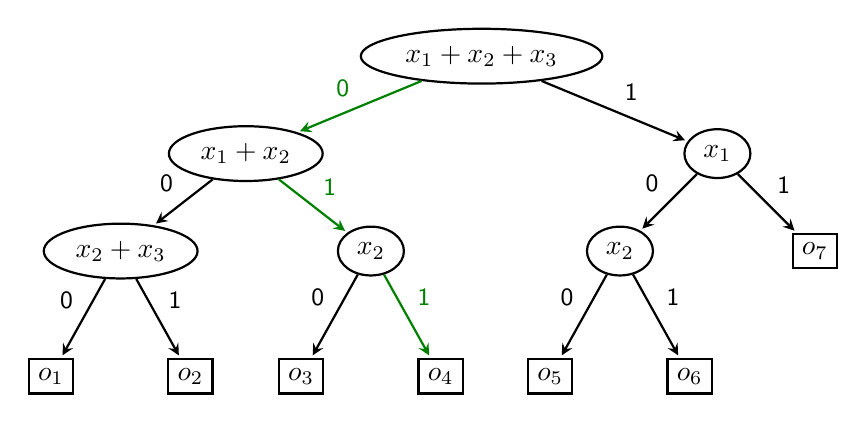
\begin{tikzpicture}[->,>=stealth,shorten >=1pt,auto,node distance=1.75cm, thick,main node/.style={scale=0.9,circle,draw,font=\sffamily\normalsize}]

        \node[ellipse, draw] (1)[] {$x_1+x_2+x_3$};

        \node[ellipse, draw] (2) [below left of=1, xshift=-50, ]{$x_1+x_2$};
        \node[ellipse, draw] (3) [below right of=1, xshift=50, ]{$x_1$};

        \node[ellipse, draw] (4) [below left of=2, xshift=-10, ]{$x_2+x_3$};
        \node[ellipse, draw] (5) [below right of=2, xshift=10, ]{$x_2$};
        \node[ellipse, draw] (6) [below left of=3, ]{$x_2$};
        \node[rectangle, draw] (7) [below right of=3]{$o_7$};

        \node[rectangle, draw] (8) [below left of=4, xshift=10, yshift=-10]{$o_1$};
        \node[rectangle, draw] (9) [below right of=4, xshift=-10, yshift=-10]{$o_2$};
        \node[rectangle, draw] (10) [below left of=5, xshift=10, yshift=-10]{$o_3$};
        \node[rectangle, draw] (11) [below right of=5, xshift=-10, yshift=-10]{$o_4$};
        \node[rectangle, draw] (12) [below left of=6, xshift=10, yshift=-10]{$o_5$};
        \node[rectangle, draw] (13) [below right of=6, xshift=-10, yshift=-10]{$o_6$};

        \path[every node/.style={font=\sffamily\small}]
            (1) edge[swap, color=Green]  node{0} (2)
            (1) edge node{1}(3)

            (2) edge[swap]  node{0} (4)
            (2) edge[color=Green]  node{1}(5)

            (3) edge[swap]  node{0} (6)
            (3) edge  node{1}(7)
                        
            (4) edge[swap]  node{0} (8)
            (4) edge  node{1}(9)

            (5) edge[swap]  node{0} (10)
            (5) edge[color=Green]  node{1}(11)

            (6) edge[swap]  node{0} (12)
            (6) edge  node{1}(13)
            ;
    \end{tikzpicture}

    \caption{An example of a parity decision tree of size 13 and depth 3.}
\end{figure}

In the above example, the green path defines the following system of linear forms:
\[\left \{ \begin{array}{l}
 x_1 + x_2 + x_3 = 0 \\
 x_1 + x_2 = 1 \\
 x_2 = 1
\end{array}\right .\]

which once simplified corresponds to the assignment $x_0 = 0, x_2 = 1, x_3 = 1$. We define the class $\mathsf{FP}^{pdt}$ as the set of $\mathsf{TFNP}^{dt}$ problems that are efficiently solvable by a PDT, where the complexity measures are defined as in normal decision trees.

\begin{definition}
 We define $\mathsf{FP}^{pdt}$ as the set of query search problems $R = (R_n)_{n \in \N}$ for which there exists a polylogarithmic depth PDT $T_n$ such that $T_n(x) = y$ if and only if $(x,y) \in R_n$.
\end{definition}

It's easy to see that $\mathsf{FP}^{dt} \subseteq \mathsf{FP}^{pdt}$ since any decision tree is just a PDT with all the queries defined only on one variable. Any PDT can be converted into a normal decision tree simply by \curlyquotes{splitting} each linear query. Given a node $v$ labeled with the linear form $f + x_i$, let $u$ and $w$ be the children of $v$ respectively given by $f + x_i = 0$ and $f+x_i = 1$. Let $T_u$ and $T_w$ be the two subtrees with root $u$ and $w$.

\newpage

\begin{figure}[H]
    \centering

    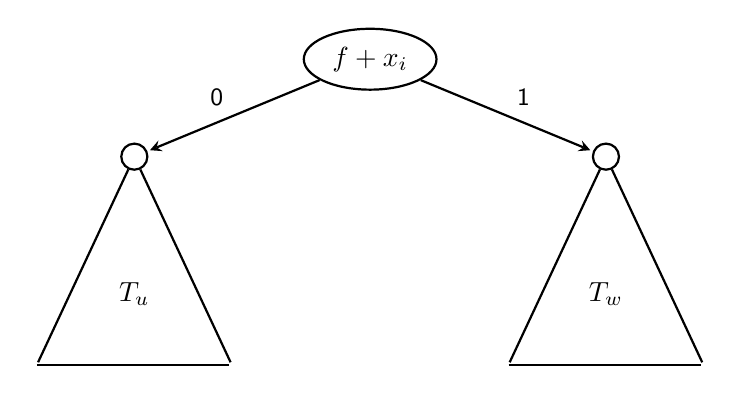
\begin{tikzpicture}[->,>=stealth,shorten >=1pt,auto,node distance=1.75cm, thick,main node/.style={scale=0.9,circle,draw,font=\sffamily\normalsize}]

        \node[ellipse, draw] (1)[] {$f + x_i$};

        \node[circle, draw] (2) [below left of=1, xshift=-50, ]{};
        \node[circle, draw] (3) [below right of=1, xshift=50, ]{};

        \node[] (2a) [below left of=2, yshift=-40]{};
        \node[] (2b) [below right of=2, yshift=-40]{};
        \node[] (2c) [below of=2]{$T_u$};

        \node[] (3a) [below left of=3, yshift=-40]{};
        \node[] (3b) [below right of=3, yshift=-40]{};
        \node[] (3c) [below of=3]{$T_w$};

        \path[every node/.style={font=\sffamily\small}]
            (1) edge[swap]  node{0} (2)
            (1) edge node{1}(3)
            ;

        \path[every node/.style={font=\sffamily\small}, -]
            (2) edge (2a.center)
            (2) edge (2b.center)
            (2a.center) edge (2b.center)
            ;

        \path[every node/.style={font=\sffamily\small}, -]
            (3) edge (3a.center)
            (3) edge (3b.center)
            (3a.center) edge (3b.center)
            ;
    \end{tikzpicture}

    \caption{The initial subtree of a parity decision tree}
\end{figure}

We replace $v$ with the node $v'$ labeled with the linear form $x_i$ and introduce two new nodes $u', w'$ such that $u'$ is the child of $v'$ when $x_i = 0$ and $w'$ is the child of $v'$ when $x_i = 1$. We label $u'$ with the linear form $f$ and let a copy of $T_u$ be the children of $u'$ when $f = 0$, while a copy of $T_w$ is the children of $u'$ when $f = 1$. Symmetrically, we label $w'$ with the linear form $f$ and let a copy of $T_w$ be the children of $w'$ when $f = 0$, while a copy of $T_u$ is the children of $w'$ when $f = 1$. 

\begin{figure}[H]
    \centering

    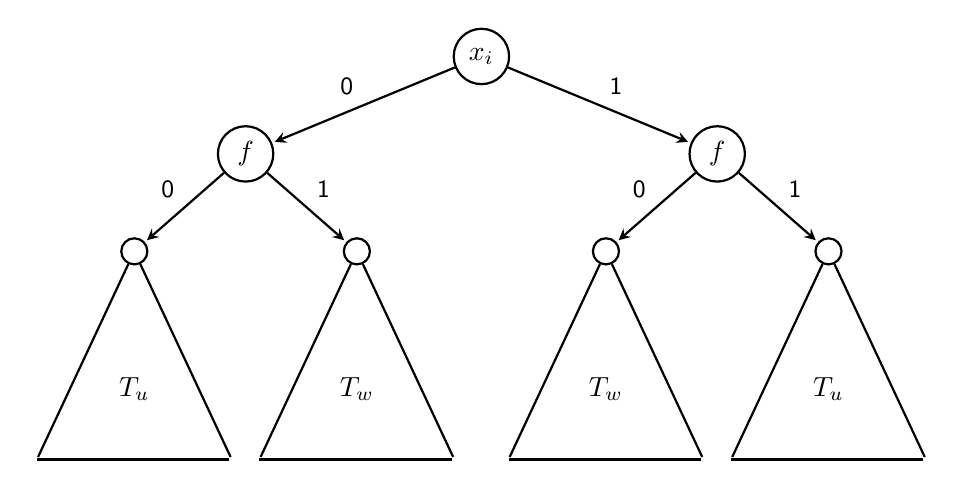
\begin{tikzpicture}[->,>=stealth,shorten >=1pt,auto,node distance=1.75cm, thick,main node/.style={scale=0.9,circle,draw,font=\sffamily\normalsize}]

        \node[circle, draw] (1)[] {$x_i$};

        \node[circle, draw] (2) [below left of=1, xshift=-50, ]{$f$};
        \node[circle, draw] (3) [below right of=1, xshift=50, ]{$f$};

        \node[circle, draw] (2x) [below left of=2, xshift=-5]{};
        \node[circle, draw] (2y) [below right of=2, xshift=5]{};

        \node[circle, draw] (3x) [below left of=3, xshift=-5]{};
        \node[circle, draw] (3y) [below right of=3, xshift=5]{};

        \node[] (2a) [below left of=2x, yshift=-40]{};
        \node[] (2b) [below right of=2x, yshift=-40]{};
        \node[] (2c) [below of=2x]{$T_u$};

        \node[] (3a) [below left of=2y, yshift=-40]{};
        \node[] (3b) [below right of=2y, yshift=-40]{};
        \node[] (3c) [below of=2y]{$T_w$};

        \node[] (4a) [below left of=3x, yshift=-40]{};
        \node[] (4b) [below right of=3x, yshift=-40]{};
        \node[] (4c) [below of=3x]{$T_w$};

        \node[] (5a) [below left of=3y, yshift=-40]{};
        \node[] (5b) [below right of=3y, yshift=-40]{};
        \node[] (5c) [below of=3y]{$T_u$};

        \path[every node/.style={font=\sffamily\small}]
            (1) edge[swap]  node{0} (2)
            (1) edge node{1}(3)

            (2) edge[swap]  node{0} (2x)
            (2) edge node{1}(2y)

            (3) edge[swap]  node{0} (3x)
            (3) edge node{1}(3y)
            ;

        \path[every node/.style={font=\sffamily\small}, -]
            (2x) edge (2a.center)
            (2x) edge (2b.center)
            (2a.center) edge (2b.center)
            ;

        \path[every node/.style={font=\sffamily\small}, -]
            (2y) edge (3a.center)
            (2y) edge (3b.center)
            (3a.center) edge (3b.center)
            ;

        \path[every node/.style={font=\sffamily\small}, -]
            (3x) edge (4a.center)
            (3x) edge (4b.center)
            (4a.center) edge (4b.center)
            ;

        \path[every node/.style={font=\sffamily\small}, -]
            (3y) edge (5a.center)
            (3y) edge (5b.center)
            (5a.center) edge (5b.center)
            ;
    \end{tikzpicture}

    \caption{The subtree after the splitting process}
\end{figure}

By repeating this process until all queries are defined on a single variable, we obtain a decision tree equivalent to the original PDT. This final decision tree has exponential size and polynomial depth, which \textit{may not} be the smallest possible decision tree that solves the search problem solved by the initial PDT. However, we can easily prove that parity decision trees are indeed much stronger than decision trees.

\begin{theorem}
    \label{fp_pdt_not_inside_fp_dt}
    $\mathsf{FP}^{dt} \subsetneq \mathsf{FP}^{pdt}$
\end{theorem}

\begin{proof}
    Any decision tree is also a parity decision tree, thus we trivially get that $\mathsf{FP}^{dt} \subseteq \mathsf{FP}^{pdt}$. Let $\mathrm{PARITY}$ be the \textit{$n$-bit parity search problem}, i.e. the problem of determining the parity of $n$ variables for a given assignment $\alpha$. This problem can be solved by a PDT of size and depth $O(1)$ by making a single query $x_1 + \ldots + x_n$, concluding that $\mathrm{PARITY} \in \mathsf{FP}^{dt}$.
    
    \begin{claim}
        Any decision tree solving $\mathrm{PARITY}$ on $n$ variables has depth $\Omega(n)$.
    \end{claim}

    \begin{proof}[Proof of the claim.]
        Suppose that $\mathrm{PARITY}$ on $n$ variables can be solved by a decision tree $T$ with depth less than $n$. We use an adversarial argument: we think of an execution
        of $T$, where some adversary answers each query of $T$ on the value of every input bit. The adversary can respond with $x_i = 0$ on all the first $n-1$ bits. Until the last bit $x_n$ is revealed, the tree has no way of determining the final output since it can either be 0 or 1 until the value of $x_n$ is revealed, concluding that it requires at least another query.
    \end{proof}
    
    By definition, $\mathsf{FP}^{dt}$ contains all the problems with a decision tree of polylogarithmic depth. Since $\mathrm{PARITY}$ requires a decision tree with depth $\Theta(n)$, we get that $\mathrm{PARITY} \notin \mathsf{FP}^{dt}$.
\end{proof}

Since a system of linear forms can have multiple solutions, many assignments could be mapped to the same output. However, some systems could also be unsatisfiable, meaning that the node is unreachable by any assignment. When this happens we say that the node is \textbf{degenerate}.

Like normal decision trees, PDTs can be used to solve the false clause search problem associated with any unsatisfiable CNF. A parity decision tree for a CNF formula $F$ is a PDT defined on the same variables of $F$ where for each leaf $v$ one of the following conditions holds:
\begin{enumerate}[itemsep=0em]
    \item The leaf is \textit{degenerate}
    \item The leaf \textit{refutes} a clause $C$ of $F$, meaning that the system $\Phi_v^T$ is satisfiable and every one of its solutions falsifies $C$
    \item The leaf \textit{satisfies} a clause $C$ of $F$, meaning that the system $\Phi_v^T$ has only one solution and it also satisfies $C$
\end{enumerate}

\begin{figure}[H]
    \centering

    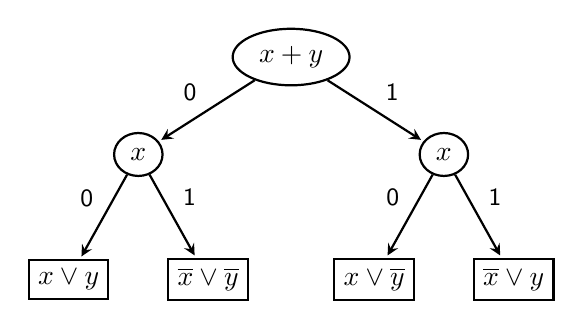
\begin{tikzpicture}[->,>=stealth,shorten >=1pt,auto,node distance=1.75cm, thick,main node/.style={scale=0.9,circle,draw,font=\sffamily\normalsize}]

        \node[ellipse, draw] (1)[] {$x + y$};

        \node[ellipse, draw] (2) [below left of=1, xshift=-20, ]{$x$};
        \node[ellipse, draw] (3) [below right of=1, xshift=20, ]{$x$};

        \node[rectangle, draw] (4) [below left of=2, xshift=10, yshift=-10]{$x \lor y$};
        \node[rectangle, draw] (5) [below right of=2, xshift=-10, yshift=-10]{$\lnot x \lor \lnot y$};
        \node[rectangle, draw] (6) [below left of=3, xshift=10, yshift=-10]{$x \lor \lnot y$};
        \node[rectangle, draw] (7) [below right of=3, xshift=-10, yshift=-10]{$\lnot x \lor y$};

        \path[every node/.style={font=\sffamily\small}]
            (1) edge[swap]  node{0} (2)
            (1) edge node{1}(3)

            (2) edge[swap]  node{0} (4)
            (2) edge[]  node{1}(5)

            (3) edge[swap]  node{0} (6)
            (3) edge  node{1}(7)
                        
            ;
    \end{tikzpicture}

    \caption{A parity decision tree for $(x \lor y) \land (\lnot x \lor \lnot y) \land (\lnot x \lor y) \land (x \lor \lnot y)$}
\end{figure}

We observe that if a node doesn't meet any of the previous conditions then it cannot be a leaf node. Moreover, we also observe that the system associated with the root of any PDT is always satisfiable due to it containing no linear forms. Since we are interested in studying PDTs for refusing unsatisfiable CNF formulas, the third case will never be true for any leaf. However, we still need a way to exclude the first case since an unsatisfiable system cannot be associated with any assignment. Luckily, each degenerate PDT can be conveniently converted into a non-degenerate one through a very simple process \cite{res_lin_2}.

\begin{proposition}
    \label{degenerate}
 Let $F$ be an unsatisfiable CNF formula. If $S_F$ can be solved with a degenerate PDT of size $s$ and depth $d$, it can also be solved with a non-degenerate PDT of size at most $s$ and depth at most $d$.
\end{proposition}

\begin{proof}
    
 Let $T$ be a degenerate PDT of size $s$ and depth $d$ that solves $S_F$. Let $U$ be the set of degenerate nodes of $T$. Notice that since $\Phi_r^T$ is empty, thus always satisfiable, we know that $r \notin U$. Consider the node $u \in U$ with the minimal distance from the root $r$. Since $u$ is not the root of $T$, there must be two vertices $p$ and $s$ such that $p$ is the parent of $u$ and $s$ is the sibling of $u$.

 We notice that $\Phi_s^T$ must be satisfiable: if we assume that this is not true then both $\Phi_s^T$ and $\Phi_u^T$ would be unsatisfiable, which can be true only if $\Phi_p^T$ is also unsatisfiable, but we chose $w$ as the node in $U$ with minimal distance. Since $\Phi_s^T$ is satisfiable, the label $f = \alpha$ on the edge $(p,s)$ must be already implied $\Phi_p^T$, meaning that each assignment that satisfies $\Phi_p^T$ also satisfies $\Phi_s^T$.

 We construct a new PDT $T'$ by removing the subtree $T_u$ with root $u$ from the initial PDT $T$ and by contracting the edge $(p,s)$, merging the two nodes $p$ and $s$ into a single node $v$. In other words, the subtree $T_u$ gets removed and the children of $s$ become the new children of $p$. Each assignment that satisfies $\Phi_p^T$ also satisfies $\Phi_s^{T'}$, concluding that $T'$ also solves $S_F$. By repeating the process until $U$ is empty, we get a non-degenerate PDT that solves $S_F$ of size at most $s$ and depth at most $d$.
\end{proof}

\section{Linear Resolution over $\F_2$}

Once we have defined the class $\mathsf{FP}^{pdt}$, we are interested in finding a proof system that characterizes it. Consider a system $\Phi$ of linear forms defined on $\F_2$. This system can be viewed as the conjunction of the linear forms that it describes:
\[\left \{ \begin{array}{c}
 f_1 = \alpha_1 \\
 f_2 = \alpha_2 \\
    \vdots \\
 f_k = \alpha_k
\end{array}\right . \iff (f_1 = \alpha_1) \land (f_2 = \alpha_2) \land \ldots \land (f_k = \alpha_k)\]

\noindent
We can rewrite these conjunctions as a negation of a disjunction:
\[\bigwedge_{i = 1}^k (f_i = \alpha_i) \iff \lnot \bigvee_{i = 1}^k \lnot (f_i = \alpha_i) \iff \lnot \bigvee_{i = 1}^k (f_i = 1 + \alpha_i)\]

\noindent
which implies that the negation of the system is equivalent to a set of disjunctions:
\[\lnot \bigwedge_{i = 0}^k (f_1 = \alpha_1) \iff \bigvee_{i = 0}^k (f_1 = 1 + \alpha_1)\]

\noindent
We define such a set of disjunctions as a \textbf{linear clause}. More generally, a \textit{linear CNF formula} over $\F_n$ is a conjunction of linear clauses defined on $\F_n$.

\begin{definition}
 A linear CNF formula is a conjunction of $m$ disjunctions of linear equations over $\F_n$.
    \[\bigwedge_{i = 1}^m \bigvee_{j = 1}^{k_i} (f_j = \alpha_j)\]
\end{definition}

Linear CNF formulas can assume a complex structure such as the following:
\[((x_1+x_2 = 0) \lor (x_1 = 1)) \land ((x_2 + x_3 + x_4 = 3) \lor (x_2 + x_4 = 0))\]

We define \textbf{Linear Resolution over $\F_n$} (or $\mathsf{ResLin(\F_n)}$), an extension of standard Resolution (see \Cref{chap:bb-tfnp}) based on the following two rules:
\begin{enumerate}
    \item \textit{Resolution rule}: given two linear clauses $(f = 0) \lor C$ and $(f = 1) \lor D$ defined on $\F_n$, we can derive the linear clause $C \lor D$
    \item \textit{Weakening rule}: given a linear clause $C$, we can derive any linear clause $D$ such that $C \implies D$.
\end{enumerate}

Like in normal Resolution, in $\mathsf{ResLin(\F_n)}$ any derivation of a linear clause $C$ from a linear CNF $F$ is a sequence of linear clauses that ends with $C$, where every clause is either an axiom of $F$ or it can be derived from previous clauses through one of the two derivation rules. A linear CNF is unsatisfiable if and only if the empty linear clause can be derived from it. 

Any standard CNF formula can be described as a linear CNF formula over $\F_2$ simply by treating each clause as a disjunction of linear forms made of a single term. For example, the CNF $(x_1 \lor \lnot{x_2}) \land (\lnot{x_3} + x_1)$ can be written as the following linear CNF formula:
\[((x_1 = 1) \lor (x_2 = 0)) \land ((x_3 = 0) \lor (x_1 = 1))\]

We call this the \textit{linear encoding} of a CNF. From now on, we will restrict our interests to Linear Resolution over $\F_2$, also called \textit{parity Resolution} (or $\mathsf{Res}_\oplus$).

The weakening rule makes this proof system powerful thanks to how semantical implications can be used as \curlyquotes{shortcuts}. For example, consider the following linear CNF:
\[(x = 1) \land (x+y = 1) \land ((x = 0) \lor (y = 1))\]

\noindent
By rewriting the last linear clause as a negation of a conjunction, we notice that:
\[(x = 0) \lor (y = 1) \equiv \lnot ((x = 1) \land (y = 0))\]

\noindent
By simple substitution, we get that:
\[\lnot ((x = 1) \land (y = 0)) \implies  \lnot ((x = 1) \land (x+y = 1))\]

\noindent
which is equivalent to:
\[\lnot ((x = 1) \land (x+y = 1)) \equiv (x = 0) \lor (x+y = 0)\]

\noindent
concluding that $(x = 0) \lor (y = 1) \models (x = 0) \lor (x+y = 0)$. Proceeding with the resolution rule, we get the following Tree-like refutation.
\begin{figure}[H]
    \centering
    
    \begin{tikzpicture}[->,>=stealth,shorten >=1pt,auto,node distance=2.25cm, thick,main node/.style={scale=0.9,circle,draw,font=\sffamily\normalsize}]
    
        \node (1) []{$\bot$};
        
        \node (3) [above right of=1]{$(x = 0)$};
    
        \node (6) [above right of=3]{$(x=0) \lor (x+y = 0)$};
        
        \node (8) [above of=6]{$(x = 0) \lor (y = 1)$};
    
        \node (14) at ($(8)+(-4,0)$){$(x+y=1)$};
        \node (15) [left of=14]{$(x=1)$};
    
        \path[every node/.style={font=\sffamily\small}]
            (14) edge (3)
            (15) edge (1)
               
            (8) edge (6)
               
            (6) edge (3)
               
            (3) edge (1)
            ;
    \end{tikzpicture}

    \caption{$\mathsf{TreeRes}_\oplus$-proof of the previous linear CNF formula}
    \label{treelike_proof}
\end{figure}

It was shown that the weakening rule can be simulated through these simple three rules \cite{res_lin_2}:
\begin{enumerate}
    \item \textit{Simplification rule}: given a linear clause $C \lor (0 = 1)$, we can derive the linear clause $C$
    \item \textit{Syntactic weakening}: given a linear clause $C$, we can derive the linear clause $C \lor (f = \alpha)$
    \item \textit{Addition rule}: given a linear clause $C \lor (f = \alpha) \lor (g = \beta)$, we can derive the linear clause $C \lor (f = \alpha) \lor (g = \beta)$
\end{enumerate}

\begin{proposition}
 Any clause obtainable through the weakening rule can also be obtained through a sequence of applications of the previous three rules and vice versa.
\end{proposition}

This result makes working with the weakening rule easier: any clause $D$ derived through $k$ applications of these three rules starting from a clause $C$ is automatically a weakening of $C$, implying that we can replace those $k$ applications with one single use of the weakening rule.

\section{Characterization of $\textsf{FP}^{pdt}$ through $\mathsf{TreeRes}_\oplus$}

$\mathsf{TreeRes}_\oplus$ proofs and parity decision trees can be viewed as two sides of the same coin. Any tree-like $\ResP$ refutation of a linear CNF $F$ can be used to construct an (almost) equivalent PDT that solves $S_F$ and vice versa \cite{res_lin_2}.

\begin{lemma}
    \label{resp_to_pdt}
 Let $F$ be a linear CNF formula. If there is a $\mathsf{TreeRes}_\oplus$ refutation of $F$ with size $s$ and depth $d$, there also is a PDT of size at most $s$ and depth at most $d$ that solves $S_F$.
\end{lemma}

\begin{proof}
 Let $T$ be the proof tree that refutes $F$. We label each edge of $T$ whose associated clauses involve a resolution rule, while all the other weakening edges remain unlabeled. In particular, if a resolution rule is applied to the clauses $(f = 0) \lor D_1$ and $(f = 1) \lor D_2$ obtaining the clause $D_1 \lor D_2$, we label the edge from the first to the third with $f = 1$, while the other edge is labeled with $f = 0$.

 By induction on the depth of a vertex of $T$, we show that the clause written in $v$ contradicts the system $\Phi_v^T$. The root node contains the empty clause and is labeled by an empty system, making the statement trivially true. Assume now that the statement holds for a generic node $v$. We have to show that the hypothesis also holds for its children $u$ and $w$.

 Suppose that $v$ is the result of a resolution rule application, where $D_1 \lor D_2$ is the clause inside $v$. Assume that $u$ is the node that contains $(f = 0) \lor D_1$ while $w$ contains $(f = 1) \lor D_2$. By inductive hypothesis, we know that $D_1 \lor D_2$ contradicts the system $\Phi_v^T$. This means that the set of equalities in $D_1$ contradicts $\Phi_v^T$. Moreover, we know that $\Phi_u^T = \Phi_v^T \land (f = 1)$, concluding that $(f = 0) \lor D_1$ contradicts $\Phi_u^T$. Likewise, we can show that $(f = 1) \lor D_2$ contradicts $\Phi_w^T$.
    
 Suppose now that $v$ is the result of a weakening rule, where $u$ is the only child. Since $(v,u)$ is unlabeled, we get that $\Phi_v^T = \Phi_u^T$. Furthermore, since $v$ is the result of a weakening applied to $u$, we know that the clause in $u$ semantically implies the clause in $v$, but by inductive hypothesis we know that the clause in $v$ contradicts the system $\Phi_v^T$, meaning that $u$ must also contradict the system $\Phi_v^T = \Phi_u^T$. Finally, if $v$ is a leaf then the statement is trivially true since it refutes a clause of $F$.

 By contracting all the unlabeled edges given by the weakening rules, we get a parity decision tree that solves $S_F$. Due to this final step, the size of the PDT is at most $s$ and its depth is at most $d$. 
\end{proof}

\begin{figure}[H]
    \centering

    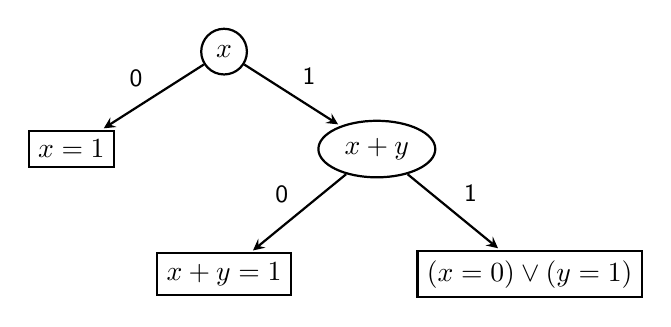
\begin{tikzpicture}[->,>=stealth,shorten >=1pt,auto,node distance=1.75cm, thick,main node/.style={scale=0.9,circle,draw,font=\sffamily\normalsize}]

        \node[circle, draw] (1)[] {$x$};

        \node[rectangle, draw] (2) [below left of=1, xshift=-20, ]{$x = 1$};
        \node[ellipse, draw] (3) [below right of=1, xshift=20, ]{$x+y$};

        \node[rectangle, draw] (4) [below left of=3, xshift=-20, yshift=-10]{$x+y = 1$};
        \node[rectangle, draw] (5) [below right of=3, xshift=20, yshift=-10]{$(x = 0) \lor (y = 1)$};

        \path[every node/.style={font=\sffamily\small}]
            (1) edge[swap]  node{0} (2)
            (1) edge node{1}(3)

            (3) edge[swap]  node{0} (4)
            (3) edge[]  node{1}(5)            
            ;
    \end{tikzpicture}

    \caption{The PDT obtained from the proof shown in \Cref{treelike_proof}}
    \label{pdt_cnf}
\end{figure}

\begin{lemma}
    \label{pdt_to_resp}
 Let $F$ be a linear CNF formula. If there is a PDT of size $s$ and depth $d$ that solves $S_F$, there also is a $\mathsf{TreeRes}_\oplus$ refutation of $F$ with size at most $2s$, depth at most $d+1$ and the weakening rule applied only to the axioms.
\end{lemma}

\begin{proof}
 Let $T$ be a PDT of size $s$ and depth $d$ that solved $S_F$. By \Cref{degenerate}, we assume that $T$ is non-degenerate. We label every node $v$ of $T$ with the negation of its associated linear system. In other words, every node $v$ is labeled with the linear clause $\lnot \Phi_v^T$. Every node is the result of the resolution rule being applied to its children, where the root node is the empty clause.

 Since $T$ is a PDT that solves $S_F$, each leaf refutes a linear clause of $F$. Hence, for each leaf $u$ we have that $\Phi_{u}^T \implies \lnot C$ for some linear clause $C$ of $F$, which equivalently means that $C \implies \lnot \Phi_u^T$, concluding that the linear clause of each leaf is actually the weakening of a clause of $F$. Then, for each leaf $u$ we can add a new neighbor node $w$ and label it with the clause $C$, where the edge $(w,u)$ becomes an application of the weakening rule. This process increases the depth of the tree by 1 and increases the size by at most $s$.
\end{proof}

\begin{figure}[H]
    \centering
    
    \begin{tikzpicture}[->,>=stealth,shorten >=1pt,auto,node distance=2.25cm, thick,main node/.style={scale=0.9,circle,draw,font=\sffamily\normalsize}]
    
        \node (1) []{$\bot$};
        
        \node (3) [above right of=1, xshift = 50]{$(x = 0)$};
    
        \node (4) [above left of=3, xshift = -20]{$(x=0) \lor (x+y = 1)$};

        \node (6) [above right of=3, xshift = 20]{$(x=0) \lor (x+y = 0)$};

        
        \node (8) [above of=6]{$(x = 0) \lor (y = 1)$};
    
        \node (14) [above of = 4]{$(x+y=1)$};
        \node (15) [left of=14, xshift = -50]{$(x=1)$};
    
        \path[every node/.style={font=\sffamily\small}]
            (14) edge (4)
            (15) edge (1)
               
            (8) edge (6)
               
            (4) edge (3)
            (6) edge (3)
               
            (3) edge (1)
            ;
    \end{tikzpicture}

    \caption{$\mathsf{TreeRes}_\oplus$-proof obtained from the PDT shown in \Cref{pdt_cnf}}
\end{figure}

We conclude that problems efficiently solvable parity decision trees are indeed characterized by Tree-like Linear Resolution over $\F_2$.

\begin{theorem}
    $\mathsf{FP}^{pdt}(S_F) = \Theta(\mathsf{TreeRes}_\oplus(F))$
\end{theorem}

After defining the class $\mathsf{FP}^{pdt}$ and proving that $\mathsf{TreeRes}_\oplus$ characterizes it, we're interested in studying where this class lies in the \textsf{TFNP}$^{dt}$ hierarchy. It's a well-known fact that $\mathsf{TreeRes}_\oplus$ can efficiently simulate $\mathsf{TreeRes}$ but the reverse doesn't hold due to the hardness of simulating weakening rules. This result also follows more naturally from our results since $\mathsf{FP}^{dt} \subsetneq \mathsf{FP}^{pdt}$. Parity makes PDTs stronger than decision trees, but how much stronger?

We know that Tree-like Linear Resolution over $\F_2$ is based on linear forms defined on $\F_2$. Since Nullstellensatz over $\F_2$ also works with polynomials over $\F_2$, our intuition was to show that these two proof systems are somehow related to one another. Initially, our first hypothesis was that $\mathsf{TreeRes}_\oplus$ is a very powerful tool even capable of efficiently simulating $\mathrm{\F_2\text{-}NS}$. We tried to prove this result by showing that $\mathsf{PPA}^{dt} \subseteq \mathsf{FP}^{pdt}$, which appeared to be out of reach.

In a seminal paper \cite{res_lin_2}, Itsykson and Sokolov discussed how $\mathsf{TreeRes}_\oplus$ cannot efficiently simulate regular Resolution (or $\mathsf{RegRes}$), a restricted proof system derived from Resolution. Due to any regular Resolution proof also being a Resolution proof, this result also implies that $\mathsf{TreeRes}_\oplus$ cannot efficiently simulate $\mathsf{Res}$. Thanks to \Cref{equiv_proof} and the fact that $\mathrm{PLS}^{dt}(S_F) = \Theta(\mathsf{Res}(F))$, we conclude the following black-box separation.

\begin{proposition}
    \label{pls_not_inside_fp_pdt}
    $\mathsf{PLS}^{dt} \not\subseteq \mathsf{FP}^{pdt}$
\end{proposition}

\newpage

This separation rings a bell: looks like PDTs aren't actually that strong. We quickly shifted our perspective on our previous study on relationships with Nullstellensatz, trying to show that the simulation holds in the other direction. Indeed, we were capable of proving that any $\mathsf{TreeRes}_\oplus$ can be converted into a small $\mathrm{\F_2\text{-}Nullstellensatz}$ proof, providing us a \textbf{black-box inclusion} for our new class.

\section{Nullstellensatz over $\F_2$}

In 1893, the mathematician Hilbert proved a theorem that established the basis of algebraic geometry, a field that studies the relations between algebra and geometry. This theorem is now known as Hilbert's \textbf{Nullstellensatz} (german for \textit{zero-locus theorem}).

The \textit{weak Nullstellensatz}, a corollary of the stronger theorem, states that given $m$ polynomials $p_1, \ldots, p_m$ defined on $F[x_1, \ldots, x_n]$, where $\F$ is a generic algebraic field, the system $p_1(x) = p_2(x) = \ldots = p_m(x) = 0$ is unsolvable if and only if there are $m$ polynomials $g_1, \ldots, g_m$ defined on $F[x_1, \ldots, x_n]$ such that $\sum_{i=1}^m g_ip_i = 1$.

This weaker version of the theorem has been used to define an \textit{algebraic} proof system, that being a proof system based on polynomial algebra. Intuitively, these proof systems are based on the idea of showing that a set of polynomials $p_1, \ldots, p_m$, called \textit{axioms}, doesn't share a common root, which serves as a proof for the polynomials. In this case, a Nullstellensatz proof is given by the set of polynomials $g_1, \ldots, g_m$ through which we get that $\sum_{i=1}^m g_ip_i = 1$  \cite{ns_definitions}. 

Any CNF formula can be translated to an \textit{algebraic encoding}, a set of polynomials $p_1, \ldots, p_m$ for which the CNF formula is unsatisfiable if and only if there is a Nullstellensatz proof for $p_1, \ldots, p_m$. Given the clause $C = \bigvee_{i = 1}^k x_i \lor \bigvee_{j = 1}^h \lnot y_j$, the algebraic encoding of $C$, written as $p_C$, is given by $p_C := \prod_{i = 1}^{k} x_i \cdot \prod_{j = 1}^h (1- y_j)$. 

To clear things up, we notice that through this formulation the concept of truthfulness is \textbf{inverted}: the boolean values $0$ and $1$ respectively correspond to the algebraic values $1$ and $0$. For example, the boolean clause $C$ evaluates to 1 when at least a literal inside it evaluates to 1, while an algebraic clause evaluates to 0 when at least a literal inside it evaluates to 0.

The algebraic encoding of a CNF formula $F = C_1 \land \ldots \land C_m$ is given by the set of polynomial equations $p_F = \{p_{C_1} = 0, \ldots, p_{C_m} = 0, x_1^2-x_1 = 0, \ldots, x_n^2-x_n = 0\}$. These last polynomials are necessary to impose that the values of $x_1, \ldots, x_n$ are either a 0 or a 1. A Nullstellensatz \textit{refutation} for $F$ is given by the polynomials $g_1, \ldots, g_m, h_1, \ldots, h_n$ such that:
\[\sum_{i = 1}^m g_ip_{C_i} + \sum_{j = 1}^m h_j(x_j^2-x_j) = 1\]
In order for the CNF $F$ to be satisfied by an assignment $x$, each clause must evaluate to 1, while in Nullstellensatz the polynomials inside $p_F$ must all evaluate to 0. 

\begin{figure}[H]
    \centering
    \begin{tabular}{r c l}
 0 & $\longrightarrow$ & 1 \\
 1 & $\longrightarrow$ & 0 \\
        $x_i$ & $\longrightarrow$ & $x_i$ \\
        $\lnot x_i$ & $\longrightarrow$ & $1-x_i$ \\
        $C \lor D$ & $\longrightarrow$ & $C \cdot D$ \\
        $C \land D$ & $\longrightarrow$ & $C + D$ \\
    \end{tabular}

    \caption{Mappings from boolean encoding to algebraic encoding}
\end{figure}

When a polynomial $q$ can be derived from a set of axioms $P$, we write $P \stackrel{\mathsf{NS}}{\vdash} q$. If $F$ is a CNF formula and $P \stackrel{\mathsf{NS}}{\vdash} 1$ then we get a Nullstellensatz refutation.

Consider the following CNF formula:
\[x_1 \land (\lnot x_1 \lor x_2) \land (\lnot x_2 \lor x_3) \land (\lnot x_3 \lor x_4)\land x_4\]
The algebraic encoding is given by $p_1 = x_1$, $p_i = (1-x_{i-1})x_i$ when $2 \leq i \leq 4$ and $p_5 = 1-x_4$. To refute this CNF, we must find the polynomials $g_1, \ldots, g_5, h_1, \ldots, h_4$ through which
\[\sum_{i = 1}^5 g_ip_{i} + \sum_{j = 1}^4 h_j(x_j^2-x_j) = 1\]

\noindent
To simplify things, we let $h_1, \ldots, h_4 = 0$ in order to have $\sum_{j = 1}^4 h_j(x_j^2-x_j) = 0$. Let $g_1, \ldots, g_5$ be equal to:
\[\begin{split}
 g_1 &= x_2x_3x_4 \\
 g_2 &= x_3x_4 \\
 g_3 &= x_4 \\
 g_4 &= 1 \\
 g_5 &= 1 \\
\end{split}\]

\noindent
We easily get that:
\[\begin{split}
    \sum_{i = 1}^5 g_ip_{i}&= x_1x_2x_3x_4 + (1-x_1)x_2x_3x_4 + (1-x_2)x_3x_4 + (1-x_3)x_4 + (1-x_4)\\
    &= x_2x_3x_4 + (1-x_2)x_3x_4 + (1-x_3)x_4 + (1-x_4)\\
    &= x_3x_4 + (1-x_3)x_4 + (1-x_4)\\
    &= x_4 + (1-x_4)\\
    &= 1\\
\end{split}\]
concluding that $P_F \stackrel{\mathsf{NS}}{\vdash} 1$ and thus proving that the CNF is unsatisfiable. In Nullstellensatz, the \textit{size} of a proof is the total number of monomials of the polynomials that make the proof, i.e. the total number of terms in the sum once fully expanded without simplifying any addition (or subtraction). The \textit{degree} of the proof is the maximum degree of any polynomial $g_ip_i$ or $h_j(x^j+x_j)$. For example, the polynomial $(1-x_1)(1-x_2)x_2x_3$ has size 4 and degree 4 since $(1-x_1)(1-x_2)x_2x_3 = x_2x_3 - x_2^2x_3 - x_1x_2x_3 + x_1x_2^2x_3$. The previous proof has size $1+2+2+2+2 = 9$ and degree $4$.

Nullstellensatz's degree measure vaguely resembles Resolution's width measure. For example, the algebraic encoding of a CNF clause $C$ of width $w$ clearly has degree $w$. Moreover, it's easy to see that a degree upper bound $d$ for the Nullstellensatz refutation of a CNF formula defined on $n$ variables implies a size upper bound of $n^{O(d)}$. This result enables us to restrict our interest to the degree of the proof.

\begin{proposition}
    \label{degree_size}
 Given a CNF formula $F$ defined on $n$ variables, if $P_F \stackrel{\mathsf{NS}}{\vdash} 1$ with degree $O(d)$ then the size of the proof is $n^{O(d)}$.
\end{proposition}

A common result shows that in Nullstellensatz proofs we can assume that polynomials are \textit{multilinear} (short for \textit{multivariate and linear}), meaning that each variable of each term has algebraic multiplicity equal to at most. For example, the polynomial $xy+yz$ is multilinear, while $x^2y$ isn't. This assumption affects the size and the degree of the proof only by a constant factor, which is negligible, allowing us to work easier.

As shown in \Cref{TFNP_dt_hierarchy}, $\F_2$-Nullstellensatz characterizes the black-box version of the class $\mathsf{PPA}$, the class of total search problems that are reducible to the \textbf{Polynomial Parity Argument (PPA)}, first defined by Papadimitriou \cite{PPA_complexity}. These problems have a solution guaranteed by the \textit{Handshaking lemma}: every undirected graph with an odd-degree node must have another odd-degree node. Papadimitriou defined the completeness of this class through the $LEAF$ problem, which asks the question \say{given a leaf of a graph, find another leaf on such graph}.

Through \Cref{equiv_proof}, we know that an efficient proof for a formula $F$ directly implies that its search problem $S_F$ is actually efficiently reducible to the black-box version of the $\mathrm{LEAF}$ problem. In the following section, we show how to convert an efficient $\mathrm{TreeRes}_\oplus$ into an efficient $\F_2$-Nullstellensatz proof, proving that each problem efficiently solvable through a PDT is reducible to an instance of $\mathrm{LEAF}^{dt}$, which implies that $\mathsf{FP}^{pdt} \subseteq \mathsf{PPA}^{dt}$.

\section{From $\mathsf{TreeRes}_\oplus$ to $\F_2$-Nullstellensatz}

We prove that Nullstellensatz over $\F_2$ is capable of efficiently simulating $\mathrm{TreeRes}_\oplus$. Given the linear clause $C = \bigvee_{i = 1}^k (f_i = \alpha_i)$, the algebraic encoding of $C$, written as $p_C$, is given by $p_C := \prod_{i = 1}^{k} (f_i + a_i)$. The algebraic encoding of a linear CNF formula $F = C_1 \land \ldots \land C_m$ is given by the set of polynomial equations $p_F = \{p_{C_1} = 0, \ldots, p_{C_m} = 0, x_1^2-x_1 = 0, \ldots, x_n^2-x_n = 0\}$.

To achieve our result, we first convert the $\mathrm{TreeRes}_\oplus$ proof into an (almost) equivalent proof through the method shown in \Cref{chap:parity-tfnp} and then balance the degree of the $\mathsf{\F_2-NS}$ proof obtained from the tree-like proof. The following result follows from \Cref{resp_to_pdt} and \Cref{pdt_to_resp}.

\begin{corollary}
    \label{leaf_weakening}
 Every $\mathsf{TreeRes}_{\oplus}$ proof of size $s$ and depth $d$ can be converted to a $\mathsf{TreeRes}_{\oplus}$ proof of size $O(s)$, degree $O(d)$ and with the weakening rule applied only to the axioms.
\end{corollary}

Next, we prove some basic Nullstellensatz inspired by the ones shown in \cite{groebner}, which allow us to manipulate and combine different types of proofs. We will use these properties to inductively simulate the resolution rule.

Given a formula $F$, we denote with $F_{\mid_{f = \alpha}}$ the formula obtained by substituting $f$ with $\alpha$ inside $F$. This is usually called \textit{restriction of $F$ on $f = \alpha$}. In particular, we notice that if $F$ is a CNF formula then by restricting it on $f = 0$ any clause $C \lor (f = 0)$ becomes $C \lor (0 = 1)$, which is equivalent to $C$ through weakening. If we restrict $F$ on $f = 1$, any clause $C \lor (f = 0)$ becomes $C \lor (1=1)$, which directly evaluates to $1$.
In a similar fashion, given the polynomial $p$ we denote with $p_{\mid_{f = \alpha}}$ the restriction of $p$ on $f = \alpha$, i.e. the polynomial obtained by setting $f$ equal to $\alpha$ in $p$.

\begin{lemma}
    \label{ns_properties}
    Given the multilinear polynomials $p_1, \ldots, p_k$ of degree at most $d$ and a linear form $f$, it holds that:
    \begin{enumerate}
        \item If $p_1, \ldots, p_k, f \vdash 1$ with degree $d$ then $p_1, \ldots, p_k \vdash 1-f$ with degree $d+1$.
        \item If $p_1, \ldots, p_k, 1-f \vdash 1$ with degree $d$ then $p_1, \ldots, p_k \vdash f$ with degree $d+1$.
        \item $p_i, f \vdash p_{i \mid_{f=0}}$ with degree $d$ 
        \item $p_i, 1-f \vdash p_{i \mid_{f=1}}$ with degree $d$ 
        \item If $p_{1\mid_{f=0}}, \ldots, p_{k\mid_{f=0}} \vdash 1$ with degree $d$ and $p_{1\mid_{f=1}}, \ldots, p_{k\mid_{f=1}} \vdash 1$ with degree $d+1$, then $p_1, \ldots, p_k \vdash 1$ with degree $d+1$
        \item If $p_{1\mid_{f=0}}, \ldots, p_{k\mid_{f=0}} \vdash 1$ with degree $d+1$ and $p_{1\mid_{f=1}}, \ldots, p_{k\mid_{f=1}} \vdash 1$ with degree $d$, then $p_1, \ldots, p_k \vdash 1$ with degree $d+1$
    \end{enumerate}
\end{lemma}

\begin{proof}
    We proceed claim by claim:
    \begin{enumerate}
        \item Since $g_{k+1}f + \sum_{i = 1}^k g_i p_i = 1$, we easily get that:
        \[(1-f)g_{k+1}f + (1-f)\sum_{i = 1}^k g_i p_i = 1-f\]
        
        Moreover, since $(1-f) f = 0$ due to it being an axiom, we can remove $f$ from the proof, concluding that $(1-f)\sum_{i = 1}^k g_i p_i = 1-f$ with degree incremented by one due to  $f$ being a linear form.
    
        \item Similar to the first claim of this lemma: multiply the whole proof by $f$ instead of $1-f$.
        
        \item Let $p = f p_1 + p_0$, where $p_1$ and $p_0$ are independent of $f$. By restricting $p$ on $f = 0$ we get that:
        \[p_{\mid_{f=0}} = 0 \cdot p_1 + p_0 = p_0 = p - f p_1\]
        Since $p$ has degree at most $d$ and $f$ has degree 1, $p_1$ must have degree at most $d-1$, thus $p - f p_1 = p_{\mid_{f=0}}$ is a proof of degree at most $d$.
        
        \item Similar to the third claim of this lemma: by restricting $p$ on $f=1$ we obtain that:
        \[p_{\mid_{f=1}} = p_1 + p_0 = p_1 + p_0 + fp_1 - fp_1 = p+(1-f)p_1\]
        thus $p + (1-f)p_1 = p_{\mid_{f=1}}$ is a proof of degree at most $d$.

        \item Through the previous claims of this lemma $p_1, \ldots, p_k, f \vdash p_{1\mid_{f=0}}, \ldots, p_{k\mid_{f=0}} \vdash 1$ with degree $d$. Then, by the first claim of this lemma, we know that $p_1, \ldots, p_k, f \vdash  1$ with degree $d$ implies that $p_1, \ldots, p_k \vdash 1-f$ with degree $d+1$. Likewise, we have that $p_1, \ldots, p_k, 1-f \vdash p_{1\mid_{f=1}}, \ldots, p_{k\mid_{f=1}} \vdash 1$ with degree $d+1$.
        
        Finally, since $p_1, \ldots, p_k \vdash 1-f$ and $p_1, \ldots, p_k, 1-f \vdash 1$ both with degree $d+1$, by concatenating the two proofs we get that $p_1, \ldots, p_k \vdash 1$ with degree $d+1$.

        \item Similar to the third claim of this lemma: invert the roles of the two initial proofs and use the second claim of this lemma.
    \end{enumerate}
\end{proof}

\begin{lemma}
    \label{union_ref}
 Given two disjoint axiom sets $P_1, P_2$ of multilinear polynomials, if $P_1, p \vdash 1$ with degree $d_1$ and $P_2, 1-p \vdash 1$ with degree $d_2$ then $P_1, P_2 \vdash 1$ with degree $d_1 + d_2$.
\end{lemma}

\begin{proof}
 Assume that $P_1 = \{p_1, \ldots, p_m\}$ and $P_2 = \{q_1, \ldots, q_k\}$ and let $p_{m+1} = p$ and $q_{k+1} = 1-p$. Since $\sum_{i = 1}^{m+1} g_i p_i + \sum_{j = 1}^n a_j (x_j^2-x_j) = 1$ for some $g_1, \ldots, g_{m+1}$, we that:
\[\sum_{i = 1}^{m} g_i p_i + \sum_{j = 1}^n a_j (x_j^2-x_j) = 1 - g_{m+1} p_{m+1} = 1-g_{m+1} p\]
    
\noindent
 Likewise, since $\sum_{i = 1}^{k+1} h_i q_i + \sum_{j = 1}^n b_j (x_j^2-x_j) = 1$ for some $h_1, \ldots, h_{k+1}$, we get that:
\[\sum_{i = 1}^{k} h_iq_i + \sum_{j = 1}^n b_j (x_j^2-x_j) = 1-h_{k+1}q_{k+1} = 1-h_{k+1}(1-p)\]

\noindent
 We notice that:
    \[\begin{split}
 (1-p) \left (\sum_{i = 1}^{m} g_i p_i + \sum_{j = 1}^n a_j (x_j^2-x_j) \right ) &= (1-p)(1-g_{m+1} p) \\
        &= 1-g_{m+1}p- p+ g_{m+1}p^2 \\
        &= 1-p
    \end{split}\]
 with degree $d_1+d_2$. In the last step, we used the fact that $p^2 = p$ due to multilinearity. Similarly, we get that:
    \[\begin{split}
 p\left (\sum_{i = 1}^{k} h_iq_i + \sum_{j = 1}^n b_j (x_j^2-x_j)  \right ) &= p 
    \end{split}\]
 again with degree $d_1+d_2$. By summing these two proofs, we get that 
    \[(1-p) \left (\sum_{i = 1}^{m} g_i p_i + \sum_{j = 1}^n a_j (x_j^2-x_j) \right ) + p \left (\sum_{i = 1}^{k} h_iq_i + \sum_{j = 1}^n b_j (x_j^2-x_j) \right )= 1\]
 concluding that $P_1, P_2 \vdash 1$ with degree $d_1 + d_2$.
\end{proof}

Next, we prove that a Tree-like Linear Resolution over $\F_2$ can be efficiently converted into a small $\F_2$-Nullstellensatz proof. The very same proof can be used to also show that standard Tree-like Linear Resolution can be simulated by $\F_2$-Nullstellensatz, an already known result.

\begin{lemma}
    \label{treeref_no_weak}
    Let $F$ be an unsatisfiable CNF. If $T$ is $\mathsf{TreeRes}_\oplus$ refutation of $F$ of size $s$ and width $w$ that uses only the resolution rule then there is $\F_2\text{-}\NS$ refutation of $F$ of degree $w+\log_2 s$.
\end{lemma}

\begin{proof}
    Let $F = C_1 \land \ldots \land C_k$. We proceed by strong induction on the size $s$ of $T$. When $S = 1$, one of the axioms of $F$ must be the empty clause, hence $p_{C_i} \vdash 1$ for some $i$ and by extension that $p_{C_i}, \ldots, p_{C_k} \vdash 1$.

    Suppose now that $s > 1$. Let $f = 0$ and $f = 1$ be the two clauses that derive the empty clause $\bot$ in $T$. These two clauses are derived through two subtrees $T_0, T_1$ of sizes $s_0, s_1$, where $s = s_0+s_1+1$. 
    
    By restricting $T_0$ on $f = 1$, the tree $T_{0 \mid_{f = 1}}$ is a $\mathsf{TreeRes}_\oplus$ proof of the formula $C_{1 \mid_{f = 1}} \land \ldots \land C_{k \mid_{f = 1}}$ of size $s_1$. Since $T$ uses only the resolution rule, $T_0$ also does. Then, my induction, we have that $p_{C_{1 \mid_{f = 1}}}, \ldots, p_{C_{k \mid_{f = 1}}} \vdash 1$ with degree $w + \log_2 s_1$. Using a similar argument, the tree $T_{1 \mid_{f = 0}}$ produces a proof $p_{C_{1 \mid_{f = 0}}}, \ldots, p_{C_{k \mid_{f = 0}}} \vdash 1$ with degree $w + \log s_2$.

    If $s_1 < \frac{s}{2}$, then $w + \log_2 s_1 \leq w + \log_2 s - 1$. Thus, the proof $p_{C_{1 \mid_{f = 1}}}, \ldots, p_{C_{k \mid_{f = 1}}} \vdash 1$ is also a proof of degree $w + \log_2 s - 1$, while the proof $p_{C_{1 \mid_{f = 0}}}, \ldots, p_{C_{k \mid_{f = 0}}} \vdash 1$ is also a proof of degree $w + \log_2 s$. By the fifth claim of \Cref{ns_properties}, we conclude that $p_{C_i}, \ldots, p_{C_k} \vdash 1$ with degree $w + \log_2 s$.

    If $s_2 < \frac{s}{2}$, instead, we get a symmetric proof, where the role of the two proofs is swapped. By the sixth claim of \Cref{ns_properties}, we again conclude that $p_{C_i}, \ldots, p_{C_k} \vdash 1$ with degree $w + \log_2 s$.
\end{proof}

\begin{figure}[H]
    \centering

    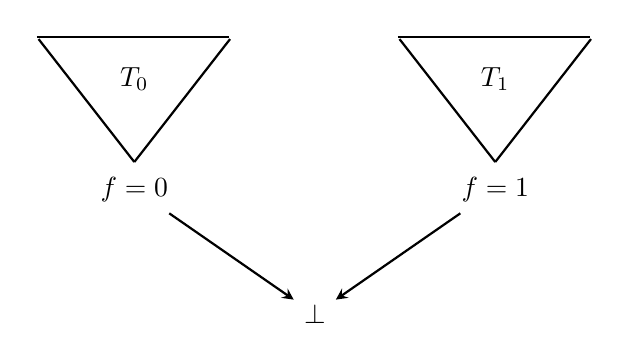
\begin{tikzpicture}[<-,>=stealth,shorten >=1pt,auto,node distance=1.75cm, thick,main node/.style={scale=0.9,circle,draw,font=\sffamily\normalsize}]

        \node[] (1) []{$\bot$};

        \node[] (2a) [above left of=1, xshift=-30, yshift=10]{$f = 0$};
        \node[] (2d) [above of=2a, yshift=-40]{};
        \node[] (2b) [above left of=2d, yshift=10]{};
        \node[] (2c) [above right of=2d, yshift=10]{};
        \node[] (2e) [above of=2a, yshift=-10]{$T_0$};

        \node[] (3a) [above right of=1, xshift=30, yshift=10]{$f = 1$};
        \node[] (3d) [above of=3a, yshift=-40]{};
        \node[] (3b) [above left of=3d, yshift=10]{};
        \node[] (3c) [above right of=3d, yshift=10]{};
        \node[] (3e) [above of=3a, yshift=-10]{$T_1$};

        \path[every node/.style={font=\sffamily\small}, -]
            (2d.center) edge (2b.center)
            (2d.center) edge (2c.center)
            (2b.center) edge (2c.center)
        ;
        
        \path[every node/.style={font=\sffamily\small}, -]
            (3d.center) edge (3b.center)
            (3d.center) edge (3c.center)
            (3b.center) edge (3c.center)
        ;

        \path[every node/.style={font=\sffamily\small}]
            (1) edge (2a)
            (1) edge (3a)
        ;

    \end{tikzpicture}

    \caption{Representation of the idea behind \Cref{treeref_no_weak}}
\end{figure}

The weakening rule is generally hard to simulate through $\F_2$-Nullstellensatz. However, if $D$ is derived through weakening from an axiom clause $C_i$ of a CNF formula $F$, we can easily simulate this rule. This result is enough for our purposes but it can also be extended to derivations from a non-axiom clause with a little blow-up in degree. 

\begin{lemma}
    \label{weakening_ns}

    Let $F = C_1 \land \ldots \land C_m$ be a CNF formula and let $D$ be a linear clause. If $C_i \implies D$ then $p_{C_i} \vdash p_D$ with degree $d+k$, where $d$ is the width of $D$ and $k$ is the width of $C_i$.
\end{lemma}

\begin{proof}
    Let $C := C_i$. Assume $C = \bigvee_{i = 1}^k (x_i = \alpha_1)$ and $D = \bigvee_{j = 1}^d (f_j = \beta_j)$. We notice that any polynomial $q(1+q)$ can be derived with degree 2 from axioms. 
        \[(y_1 + \ldots + y_t)(y_1 + \ldots y_t + 1) = \sum_{i = 1}^t y_i^2 + \sum_{i = 1}^t y_i + 2 \sum_{i \neq j} y_i y_j = \sum_{i = 1}^t y_i^2 + y_i\]
    since $2 = 0$ in $\F_2$. This implies that for each $j \in [d]$ we can derive $f_j+\beta_j+1$ with degree $d+1$.

    Since $C \implies D$, this can only happen if each $x_i + \alpha_i$ is a linear combination of $(f_1 + \beta_1 + 1), \ldots, (f_d + \beta_d + 1)$, concluding that each $p_D(x_i+\alpha_i)$ is derivable in $\F_2$-Nullstellensatz with degree $d+1$. Finally, we notice that:
        \[p_D = p_C + p_D(x_1+\alpha_1+1) + p_D(x_2+\alpha_2+1)(x_1+\alpha_1)+ \ldots + p_D(x_d+\alpha_d+1)+\prod_{i = 0}^{d-1} (x_i+\alpha_i)\]
    which is a derivation of $p_D$ from $p_{C}$ with degree $d + k$.
\end{proof}

\begin{theorem}
    Let $F$ be an unsatisfiable CNF. If $T$ is $\mathsf{TreeRes}_\oplus$ refutation of $F$ of size $s$ and width $w$ then there is $\NS$ refutation of $F$ of degree $O(w + \log s)$.
\end{theorem}

\begin{proof}
    Let $F = C_1 \land \cdots \land C_m$ and let $T$ be a $\mathsf{TreeRes}_\oplus$-proof of $F$ with size $s$ and width $w$. Through \Cref{leaf_weakening} we know that there must also be a $\mathsf{TreeRes}_\oplus$-proof of size $O(s)$ with the weakening rule applied only to the leaves. Let $\widehat{C_1}, \ldots, \widehat{C_m}$ be the linear clauses obtained through such weakening rules and let $T'$ be the subtree.

    Let $T'$ be the subtree of $T$ with root $\bot$ and leaves $\widehat{C_1}, \ldots, \widehat{C_m}$. Since $T'$ only uses the resolution rule, by \Cref{treeref_no_weak} we conclude that $p_{\widehat{C_1}}, \ldots, p_{\widehat{C_m}} \vdash 1$ with degree $O(w + \log s)$. Clearly, this also implies that $\mathrm{deg}(p_{\widehat{C_i}}) = O(w + \log s)$ for all $i$.
        
    Since each $\widehat{C_i}$ is a weakening of $C_i$, by \Cref{weakening_ns} we know that $p_{C_i} \vdash p_{\widehat{C_i}}$ with degree $O(w + \log s)$. We trivially get that $p_{C_i}, (1-p_{\widehat{C_i}}) \vdash 1$ with degree $O(w + \log s)$. Moreover, since $p_{\widehat{C_1}}, \ldots, p_{\widehat{C_m}} \vdash 1$ with degree $O(w + \log s)$, by \Cref{union_ref} we get that $p_{C_1}, p_{\widehat{C_2}}, \ldots, p_{\widehat{C_m}} \vdash 1$ with degree $O(w + \log s)$. After repeating this process for each weakening clause, we finally conclude that $p_{C_1}, \ldots, p_{C_m} \vdash 1$ with degree $O(w + \log s)$. 
\end{proof}

\begin{figure}[H]
    \centering

    \begin{tikzpicture}[->,>=stealth,shorten >=1pt,auto,node distance=1.75cm, thick,main node/.style={scale=0.9,circle,draw,font=\sffamily\normalsize}]

        \node[] (2) []{};

        \node[] (2a) [above left of=2, xshift=-50, yshift=100]{};
        \node[] (2b) [above right of=2, xshift=50, yshift=100]{};
        \node[] (2c) [below of=2, yshift=40]{$\bot$};
        \node[] (2d) [above of=2, yshift = 30]{$T$};

        \node[] (4) [above of = 2a, yshift = -37.5]{$\widehat{C_1}$};
        \node[] (5) [above of = 2a, yshift = -37.5, xshift=30]{$\widehat{C_2}$};
        \node[] (6) [above of = 2a, yshift = -37.5, xshift=60]{$\cdots$};
        \node[] (7) [above of = 2a, yshift = -37.5, xshift=85]{$\cdots$};
        \node[] (8) [above of = 2b, yshift = -37.5]{$\widehat{C_m}$};
        \node[] (9) [above of = 2b, yshift = -37.5, xshift=-30]{$\widehat{C_{m-1}}$};
        \node[] (10) [above of = 2b, yshift = -37.5, xshift=-60]{$\cdots$};


        \node[] (11) [above of = 2a]{${C_1}$};
        \node[] (12) [above of = 2a, xshift=30]{${C_2}$};
        \node[] (13) [above of = 2a, xshift=60]{$\cdots$};
        \node[] (14) [above of = 2a, xshift=85]{$\cdots$};
        \node[] (15) [above of = 2b]{${C_m}$};
        \node[] (16) [above of = 2b, xshift=-30]{${C_{m-1}}$};
        \node[] (17) [above of = 2b, xshift=-60]{$\cdots$};

        \path[every node/.style={font=\sffamily\small}, -]
            (4) edge (11)
            (5) edge (12)
            (8) edge (15)
            (9) edge (16)
            ;

        \path[every node/.style={font=\sffamily\small}, -]
            (2.center) edge (2a.center)
            (2.center) edge (2b.center)
            (2a.center) edge (2b.center)
            ;

    \end{tikzpicture}

    \caption{Representation of the idea behind \Cref{main_thm}}
\end{figure}

Finally, thanks to \Cref{equiv_proof} and the fact that $\mathrm{PPA}^{dt}(S_F) = \Theta(\F_2\text{-}\mathsf{NS}(F))$, the last theorem proves that our new class is indeed contained inside $\mathsf{PPA}^{dt}$, meaning that any total search problem efficiently solvable by a parity decision tree can be reduced to an instance of the parity argument problem.  
   
\begin{theorem}
    \label{main_thm}
    $\mathsf{FP}^{pdt} \subseteq \mathsf{PPA}^{dt}$
\end{theorem}

\begin{proof}
 Suppose that $R \in \mathsf{FP}^{pdt}$. By definition, there is a PDT that solves $R$ with size $s$ and depth $d$, where $d+\log s = O(\log^k n)$ for some $k \in \N$. We know that each $\textsf{TFNP}^{dt}$ is equivalent to the false clause search problem of some CNF formula $F$, thus $R = S_F$.
    
 By \Cref{pdt_to_resp}, we know that there is a \textsf{TreeRes}$_{\oplus}$ proof of $F$ with size $O(s)$ and depth $d$. Then, by theorem \Cref{main_thm}, we know that there must be a $\F_2$-Nullstellensatz refutation for $F$ with degree $O(w + \log s)$ and size $n^{O(w + \log s)}$, where $w$ is the width of the tree-like proof.
 
 Moreover, since $\log s = O(\log^k n)$, we have that $s = O(n^k)$, hence $F$ has a $\F_2$-\textsf{NS} refutation of degree $O(\log n)$. By \Cref{equiv_proof}, we know that there is an efficient reduction $S_F \leq_m \mathsf{PPA}^{dt}$, concluding that $R \in \mathsf{PPA}^{pdt}$
\end{proof}

% The balancing process is obtained through a well-known result called $\frac{1}{2}, \frac{2}{3}$ lemma \cite{13_23_lemma} which is commonly used to show that protocols and Tree-like circuits (also called \textit{formulas}) can be balanced, meaning that their tree structure of size $s$ can be transformed in an equivalent one of size $s^{O(1)}$ and degree $O(\log s)$.

% \begin{lemma}
%     \label{13_23_lewis}
%  If $T$ is a binary tree of size $s > 1$ then there is a node $v$ such that the subtree $T_v$ has size between $\floor{\frac{1}{3} s}$ and $\ceil{\frac{2}{3} s}$.
% \end{lemma}

% \begin{proof}
%     Let $r$ be the radix of $T$ and let $\ell$ be a leaf of $T$ with the longest possible path $r \to \ell$. Let $v_1, \ldots, v_k$ be the nodes of such path, where $r = v_1$ and $\ell = v_k$. For each index $i$ such that $1 \leq i \leq k$, let $a_i b_i$ be the two children of $v_i$.

%     \begin{claim}
%         For any index $i$, if $T_{v_i}$ has size at least $\floor{\frac{1}{3} s}$ then for some index $j$, where $i \leq j \leq k$, it holds that $T_{v_j}$ has size between $\floor{\frac{1}{3} s}$ and $\ceil{\frac{2}{3} s}$.
%     \end{claim}

%     \begin{proof}[Proof of the claim]
%         If $T_{v_i}$ has size less than $\ceil{\frac{2}{3} s}$ then we are done. Otherwise, since $T_{v_i} = \{v_i\} \cup T_{a_i} \cup T_{b_i}$, one between the subtrees $T_{a_i}, T_{b_i}$ must have size at least $\frac{1}{2} \ceil{2}{3} s - 1$, meaning that it has size at least $\floor{\frac{1}{3} s}$. If this subtree has also a size at most $\ceil{\frac{2}{3} s}$ then we are done. Instead, if this doesn't hold for both subtrees, we can repeat the process (assuming that $v_{i+1} := a_i$ without loss of generality) since we know that $T_{v_{i+1}}$ has size greater than $\floor{\frac{1}{3} s}$.

%         By way of contradiction, suppose that this process never finds a subtree with size at most $\ceil{\frac{2}{3} s}$. Then, this would mean that it also holds for $v_k = \ell$. However, since $\ell$ is a leaf, we know that $T_{v_\ell}$ must have size 1, which is definitely at most $\ceil{\frac{2}{3} s}$ for any value of $s$, giving a contradiction. Thus, there must be a node that terminates the process.
%     \end{proof}
        
%     Since $T_{v_1} = \{r\} \cup T_{a_1} \cup T_{b_1}$, we know that both of these subtrees must have size at least $\floor{\frac{1}{3} s}$. Without loss of generality, by assuming that $a_1 = v_{2}$ the claim concludes the proof of the lemma.
% \end{proof}

% We'll now show a way to simulate the resolution rule through $\F_2$-Nullstellensatz by converting two \textsf{NS} refutations $P_1 \stackrel{}{\vdash} 1$ and $P_2 \stackrel{}{\vdash} 1$, where $P_1$ and $P_2$ are disjoint, into a refutation  $P_1, P_2 \stackrel{}{\vdash} 1$ with degree equal to the degree of the two initial refutations.

% \begin{lemma}
%     \label{union_ref}
%  Given two disjoint axiom sets $P_1, P_2$, if $P_1, p \stackrel{\mathsf{NS}}{\vdash} r$ with degree $d_1$ and $P_2, 1-p \stackrel{\mathsf{NS}}{\vdash} t$ with degree $d_2$ then $P_1, P_2 \stackrel{\mathsf{NS}}{\vdash} rt$ with degree $O(d_1 + d_2)$.
% \end{lemma}

% \begin{proof}
%  Assume that $P_1 = \{p_1, \ldots, p_m\}$ and $P_2 = \{q_1, \ldots, q_k\}$ and let $p_{m+1} = p$ and $q_{k+1} = 1-p$. By hypothesis, we know that
%     \[\sum_{i = 1}^{m+1} g_i p_i + \sum_{j = 1}^n a_j (x_j^2-x_j) = r\]
%  for some $g_1, \ldots, g_{m+1}, a_1, \ldots, a_n$, implying that:
%     \[\sum_{i = 1}^{m} g_i p_i + \sum_{j = 1}^n a_j (x_j^2-x_j) = r - g_{m+1} p_{m+1} = r-g_{m+1} p\]
    
% \noindent
%  Likewise, we know that:
%     \[\sum_{i = 1}^{k+1} h_i q_i + \sum_{j = 1}^n b_j (x_j^2-x_j) = t\]
%  for some $h_1, \ldots, h_{k+1}, b_1, \ldots, b_n$, implying that:
%     \[\sum_{i = 1}^{k} h_iq_i + \sum_{j = 1}^n b_j (x_j^2-x_j) = t-h_{k+1}q_{k+1} = t-h_{k+1}(1-p)\]

% \noindent
%  We notice that:
%     \[\begin{split}
%  t(1-p) \left (\sum_{i = 1}^{m} g_i p_i + \sum_{j = 1}^n a_j (x_j^2-x_j) \right ) &= t(1-p)(r-g_{m+1} p) \\
%         &= rt-g_{m+1} tp - prt + g_{m+1} p^2t \\
%         &= rt-rtp
%     \end{split}\]
%  with degree $d_1+2d_1$. In the last step, we used the fact that due to multilinearity it holds that $p^2 = p$. Similarly, we get that:
%     \[\begin{split}
%  rp\, \left (\sum_{i = 1}^{k} h_iq_i + \sum_{j = 1}^n b_j (x_j^2-x_j)  \right ) &= rtp 
%     \end{split}\]
%  with degree $2d_1+d_1$. Let $f_1, \ldots, f_{mk}, s_1, \ldots, s_{m+k}$ be defined as:
%     \[f_i = \left \{ \begin{array}{ll}
%  p_i & \text{if } 1 \leq i \leq m \\
%  q_i & \text{if } m+1 \leq i \leq k \\
%     \end{array} \right .
%  \qquad\qquad
%  s_i = \left \{ \begin{array}{ll}
%  g_i t(1-p) & \text{if } 1 \leq i \leq m \\
%  h_irp & \text{if } m+1 \leq i \leq k \\
%     \end{array} \right .\]
%  while $c_1, \ldots, c_n$ are defined as $c_j = a_jt(1-p) + b_jrp$. Through simple algebra, we get that:
%     \[\sum_{i = 1}^{m+k} s_i f_i + \sum_{j = 1}^n c_j (x_j^2-x_j) =\]
%     \[t(1-p) \left (\sum_{i = 1}^{m} g_i p_i + \sum_{j = 1}^n a_j (x_j^2-x_j) \right ) + rp \left (\sum_{i = 1}^{k} h_iq_i + \sum_{j = 1}^n b_j (x_j^2-x_j) \right )= rt\]
%  concluding that $\Pi := \{s_1, \ldots, s_{m+k}, c_1, \ldots, c_n\}$ is a proof of $P_1 \cup P_2$ with degree $O(d_1 + d_2)$.

% \end{proof}

% \newpage

% The weakening rule is generally hard to simulate through $\F_2$-Nullstellensatz. However, if $D$ is derived through weakening from an axiom clause $C_i$ of a CNF formula $F$, it is indeed easy to simulate this rule. This result is enough for our purposes but it can also be extended to derivations from a non-axiom clause with a little blow-up in degree. 

% \begin{lemma}
%     \label{weakening_ns}

%  Let $F = C_1 \land \ldots \land C_m$ be a CNF formula and let $D$ be a linear clause. If $C_i \implies D$ then $p_{C_i} \vdash p_D$ with degree $d+k$, where $d$ is the width of $D$ and $k$ is the width of $C_i$.
% \end{lemma}

% \begin{proof}
%  Let $C := C_i$. Assume $C = \bigvee_{i = 1}^k (x_i = \alpha_1)$ and $D = \bigvee_{j = 1}^d (f_j = \beta_j)$. We notice that any polynomial $q(1+q)$ can be derived with degree 2 from axioms. 
%     \[(y_1 + \ldots + y_t)(y_1 + \ldots y_t + 1) = \sum_{i = 1}^t y_i^2 + \sum_{i = 1}^t y_i + 2 \sum_{i \neq j} y_i y_j = \sum_{i = 1}^t y_i^2 + y_i\]
%  since $2 = 0$ in $\F_2$. This implies that for each $j \in [d]$ we can derive $p(f_j+\beta_j+1)$ with degree $d+1$.

%  Since $C \implies D$, this can only happen if each $x_i + \alpha_i$ is a linear combination of $(f_1 + \beta_1 + 1), \ldots, (f_d + \beta_d + 1)$, concluding that each $p_D(x_i+\alpha_i)$ is derivable in $\F_2$-Nullstellensatz with degree $d+1$.

%  Finally, we notice that:
%     \[p_D = p_C + p_D(x_1+\alpha_1+1) + p_D(x_2+\alpha_2+1)(x_1+\alpha_1)+ \ldots + p_D(x_d+\alpha_d+1)\prod_{i = 0}^{d-1} (x_i+\alpha_i)\]
%  which is a derivation of $p_D$ from $p_{C}$ with degree $d + k$.
    
% \end{proof}

% \begin{lemma}
%     \label{refutation_with_negation}
%  Given a set of axioms $P$, if $P \stackrel{\mathsf{NS}}{\vdash} q$ with degree $d$ then $P, 1-q \stackrel{\mathsf{NS}}{\vdash} 1$ with the same degree. 
% \end{lemma}

% \begin{proof}
    
%  Since $P \vdash^\NS_d q$, we know that $\exists g_1, \ldots, g_m, h_1, \ldots, h_n \in \F[x_1, \ldots, x_n]$ such that:
%     \[\sum_{i = 1}^m g_i p_i + \sum_{j = 1}^n h_j (x_j^2-x_j) = q\]
%  where $\deg(q) \leq d$. We define $g_1', \ldots, g_m', g_{m+1}'$ as:
%     \[g_i' = \left \{ \begin{array}{ll}
%         1 & \text{if } i = m+1 \\
%  g_i & \text{otherwise}  \\
%     \end{array}\right .\]
    
% \noindent
%  With simple algebra, we get that:
%     \[\sum_{i = 1}^{m+1} g_i' p_i + \sum_{j = 1}^n h_j (x_j^2-x_j) = g_{m+1}'p_{m+1} + \sum_{i = 1}^{m} g_i' p_i + \sum_{j = 1}^n h_j (x_j^2-x_j) = (1-q) + q = 1\]
%  thus $\Pi = \{g_1', \ldots, g_{m+1}', h_1, \ldots, h_n\}$ is a proof of $P$ with degree $d$.

% \end{proof}

% \begin{theorem}
%     \label{main_thm}
%  Let $F$ be an unsatisfiable CNF. If $T$ is $\mathsf{TreeRes}_\oplus$ refutation of $F$ of size $s$ and width $w$ then there is $\NS$ refutation of $F$ of degree $O(\log(s)+w)$.
% \end{theorem}

% \begin{proof}
%  Let $F = C_1 \land \cdots \land C_m$ and let $T$ be a $\mathsf{TreeRes}_\oplus$-proof of $F$ with size $s$ and width $w$. Through \Cref{leaf_weakening} we know that there must also be a $\mathsf{TreeRes}_\oplus$-proof of size $O(s)$ with the weakening rule applied only to the leaves. Let $\widehat{C_1}, \ldots, \widehat{C_m}$ be the linear clauses obtained through such weakening rules.
    
%     \begin{claim}
%  If $T'$ is a subtree of $T$ with root $C$, leaves $D_1, \ldots, D_k$ and without nodes derived through the weakening rule then $p_{D_1}, \ldots, p_{D_k} \vdash p_C$ with degree $O(\log (s) + w)$
%     \end{claim}

%     \begin{proof}[Proof of the claim]
%  We proceed by strong induction on the size $u$ of $T'$. If $u = 1$ then the root $C$ is the only clause in $T'$, which means that it must be the only leaf in $T'$. We trivially get that $C \vdash C$ with degree $w$.
        
%  Suppose that $u > 1$. Let $\mathcal{L} = \{D_1, \ldots, D_k\}$. Since $T'$ is a binary tree, by \Cref{13_23_lewis} we know that there is a clause $Q$ (a node) inside $T'$ such that $T'_{Q}$ has size between $\floor{\frac{1}{3} u}$ and $\ceil{\frac{2}{3} u}$. Let $\overline{T_Q} = (T - T_{Q}) \cup \{Q\}$. Due to the size of $T_{Q}$, we get that $\overline{T_{Q}}$ has size between $\floor{\frac{1}{3} u}+1$ and $\ceil{\frac{2}{3} u}+1$. 
    
%  Since the proof is tree-like, $T_{Q}$ and $\overline{T_Q}$ work with different clauses (except $Q$), thus their leaves must partition $\mathcal{L}$ into two sets $\mathcal{L}_1, \mathcal{L}_2$, respectively used by $T_{Q}$ and $\overline{T_Q}$. By inductive hypothesis we get that $p_{\mathcal{L}_1} \vdash p_Q$ with degree at most $\log(s) + w$ and that $p_{\mathcal{L}_2}, p_Q \vdash p_C$ with degree at most $c_2(\log(s) + w)$, for two constants $c_1, c_2$.
        
%  Through \Cref{refutation_with_negation} we easily conclude that $p_{\mathcal{L}_1}, (1-p_{Q})\vdash 1$ with degree at most $c_1(\log(s) + w)$. Then, by \Cref{union_ref} we get that $p_{\mathcal{L}_1}, p_{\mathcal{L}_2} \vdash p_C$, thus $p_\mathcal{L} \vdash p_C$, with degree $O(\log s + w)$.
%     \end{proof}

%  Let $T'$ be the subtree of $T$ with root $\bot$ and leaves $\widehat{C_1}, \ldots, \widehat{C_m}$. Since $T'$ only uses the resolution rule, through the claim we conclude that $p_{\widehat{C_1}}, \ldots, p_{\widehat{C_m}} \vdash 1$ with degree $O(\log(s)+w)$. Clearly, this also implies that $\mathrm{deg}(p_{\widehat{C_i}}) = O(\log(s)+w)$ for all $i$.
    
%  Since each $\widehat{C_i}$ is a weakening of $C_i$, by \Cref{weakening_ns} we know that $p_{C_i} \vdash p_{\widehat{C_i}}$ with degree $O(\log(s)+ w)$. Again, by \Cref{refutation_with_negation} we get that $p_{C_i}, (1-p_{\widehat{C_i}}) \vdash 1$ with degree $O(\log(s)+ w)$ which together with the fact that $p_{\widehat{C_1}}, \ldots, p_{\widehat{C_m}} \vdash 1$ with degree $O(\log(s)+w)$ allows us to conclude, by \Cref{union_ref}, that $p_{C_1}, p_{\widehat{C_2}}, \ldots, p_{\widehat{C_m}} \vdash 1$ with degree $O(\log(s)+w)$. After repeating this process for each weakening clause, we finally conclude that $p_{C_1}, \ldots, p_{C_m} \vdash 1$ with degree $O(\log(s)+w)$.

% \end{proof}

% \newpage


% \quad

% Again, thanks to \Cref{equiv_proof} and the fact that $\mathrm{PPA}^{dt}(S_F) = \Theta(\F_2\text{-}\mathsf{NS}(F))$, the last theorem proves that our new class is indeed contained inside $\mathsf{PPA}^{dt}$, meaning that any total search problem efficiently solvable by a parity decision tree can be reduced to an instance of the parity argument problem.  

% \begin{theorem}
%     $\mathsf{FP}^{pdt} \subseteq \mathsf{PPA}^{dt}$
% \end{theorem}

% \begin{proof}
%  Suppose that $R \in \mathsf{FP}^{pdt}$. By definition, there is a PDT with size $s$ and depth $d$, where $d+\log s = O(\log^k n)$ for some $k \in \N$,that solves $R$. We know that each total search problem is equivalent to the false clause search problem of some CNF formula $F$, thus $R = S_F$.
    
%  By \Cref{pdt_to_resp}, we know that there is a \textsf{TreeRes}$_{\oplus}$ proof of $F$ with size $O(s)$. Then, by theorem \Cref{main_thm}, we know that there must be a $\F_2$-Nullstellensatz refutation for $F$ with degree $O(\log(s) + w)$, where $w$ is the width of the proof. 
    
%  Since $F$ has a $\F_2$-\textsf{NS} refutation of degree $O(\log s + w)$ and since $\mathsf{PPA}^{pdt} = \Theta(\F_2$-\textsf{NS}), by \Cref{equiv_proof} we know that there is an efficient reduction $S_F \leq_m \mathsf{PPA}^{dt}$, concluding that $R \in \mathsf{PPA}^{pdt}$

% \end{proof}

% \newpage
    

\cleardoublepage


% ================== Notes ==================


\chapter{Notes} \label{chap:notes}

\section{Treelike $\Res$ and Nullstellensatz}

\begin{definition}[$\FNS$ encoding of $\Res$]
    Given a $\Res$ linear clause $C = \bigvee\limits_{i = 0}^{k_1} x_i \lor  \bigvee\limits_{j = 0}^{k_2} \overline{x_j}$, the $\FNS$ encoding of $C$ is defined as $\enc(C) := \prod\limits_{i = 0}^{k_1} x_i \cdot \prod\limits_{j = 0}^{k_2} (1-x_j)$.
    
    In general, a $\ResP$ formula $F = C_1 \land \ldots \land C_m$ defined on the variables $x_1, \ldots, x_n$ gets encoded in $\FNS$ as the set of axioms $P_F = \{\enc(C_i) = 0 \mid 1 \leq i \leq m\} \cup \{x_j^2-x_j = 0 \mid 1 \leq j \leq n\}$.
\end{definition}

\begin{theorem}
    Let $F$ be an unsatisfiable CNF. If $T$ is $\ResP$ refutation of $F$ of size $s$ then there is $\NS$ refutation of $F$ of degree $O(\log(s))$.
\end{theorem}

\begin{proof}
    Let $F = C_1 \land \cdots \land C_n$. We proceed by strong induction on the size $s$.
    
    If $s = 1$ then the $T$ contains only the empty clause $\bot$, meaning that it also is one of the starting clauses and thus one of the axioms. We notice that $\mathrm{enc}(\bot) = 1$, which easily concludes that $\bot \vdash_{0}^\NS 1$.

    Suppose now that $s > 1$. Let $\mathcal{L}$ be axioms of $T$. Since $T$ is a binary tree, by \Cref{13_23_lewis} we know that there is a clause $C_k$, i.e. a node, of $T$ such that $T_{C_k}$ has size between $\floor{\frac{1}{3} s}$ and $\ceil{\frac{2}{3} s}$.

    Let $T' = (T - T_{C_k}) \cup \{C_k\}$. Due to the size of $T_{C_k}$, we get that $T'$ has size between $\floor{\frac{1}{3} s}+1$ and $\ceil{\frac{2}{3} s}+1$. Moreover, we notice that since $T$ is a treelike refutation it holds that $T_{C_k}$ and $T'$ work with different clauses (except $C_k$), thus their axioms are disjoint. Let $\mathcal{L}_1, \mathcal{L}_2$ be the two sets of axioms respectively used by $T_{C_k}$ and $T'$.
    
    By construction, we notice that $T_{C_k}$ derives the clause $C_k$ using the axioms $\mathcal{L}_1$, while $T_{C_k}$ derives the clause $\bot$ using the axioms $\mathcal{L}_2, C_k$. Thus, since $T_{C_k}$ and $T'$ have size lower than $s$, by induction hypothesis we get that $\enc(\mathcal{L}_1) \vdash_{c_1 \cdot \log s}^\NS \enc(C_k)$ and $\enc(\mathcal{L}_2), \enc(C_k) \vdash_{c_2 \cdot \log s}^\NS 1$ for some constants $c_1, c_2$. By \Cref{neg_refutation} we easily conclude that $\enc(\mathcal{L}_1), (1- \enc(C_k)) \vdash_{c_1 \cdot \log s}^\NS 1$ and, by \Cref{union_ref}, that $\enc(\mathcal{L}_1), \enc(\mathcal{L}_2) \vdash_{(c_1+c_2) \cdot \log s}^\NS 1$. Finally, since $\mathcal{L}_1 \cup \mathcal{L}_2 = \mathcal{L}$, we get that $\enc(\mathcal{L}) \vdash_{(c_1+c_2) \cdot \log s}^\NS 1$, meaning that $\mathcal{L}$ has a $\NS$ refutation of degree $O(\log s)$.

\end{proof}

\section{Treelike $\ResP$ and Nullstellensatz}

\begin{definition}[$\FNS$ encoding of $\Res(\oplus)$]
    Given a $\ResP$ linear clause $C = \bigvee\limits_{i = 0}^k (\ell_i = \alpha_i)$, the $\FNS$ encoding of $C$ is defined as $\enc_{\oplus}(C) := \prod\limits_{i = 0}^k (\alpha - \ell_i)$.
    
    In general, a $\ResP$ formula $F = C_1 \land \ldots \land C_m$ defined on the variables $x_1, \ldots, x_n$ gets encoded in $\FNS$ as the set of axioms $P_F = \{\enc_{\oplus}(C_i) = 0 \mid 1 \leq i \leq m\} \cup \{x_j^2-x_j = 0 \mid 1 \leq j \leq n\}$.
\end{definition}

\begin{theorem}[\cite{res_parity}]
    \;
    \begin{enumerate}
        \item Every tree-like $\ResP$ proof of an unsatisfiable formula $F$ may be translated to a parity decision tree for $F$ without increasing the size of the tree.
        
        \item Every parity decision tree for an unsatisfiable linear CNF may be translated into a tree-like $\ResP$ proof and the size of the resulting proof is at most twice the size of the parity decision tree (and where the weakening is applied only to the axioms).
    \end{enumerate}
\end{theorem}

\begin{corollary}
    Every tree-like $\ResP$ proof of an unsatisfiable formula $F$ can be converted to a tree-like $\ResP$ proof of at most double the size and with weakening applied only to the axioms.
\end{corollary}


\cleardoublepage

% ================== ACKNOWLEDGMENTS ==================
\chapter*{Acknowledgements}

    \addcontentsline{toc}{chapter}{Acknowledgements}

    this is sad, alexa play despacito
    % \noindent I am thankful to my parents, \textbf{Rodica} and \textbf{Dorin}, whose 
    % sacrifices have been the starting point of my success. The hard work and faith they have demonstrated, alongside the decision to emigrate from Romania to Italy for the sake of providing me with a brighter future, have been the driving force of my aspirations. Their love and support have been my constant source of strength.
    
    % \vspace{2mm}

    % \noindent A heartfelt thanks to my girlfriend, \textbf{Margherita}, for her enduring patience, encouragement, and love. Her belief in my capabilities and understanding during the demanding times of this degree have been invaluable. 

    % \vspace{2mm}
  
    % \noindent Last but not least, I would like to express my appreciation to my two cats, \textbf{Mimmi} and \textbf{Shelby}. Their companionship during the long nights of study has been a relief. They have been silent and sleepy witnesses to my struggles and accomplishments, their presence is a constant reminder of the importance of the little things in life.

    % \vspace{2mm}

    % \textit{To all of you, I am eternally thankful. Your contributions to my life and this work have
    % not only helped shape this academic effort but also enriched my personal growth.}

\backmatter
\phantomsection

% ================== BIBLIOGRAPHY ==================
\addcontentsline{toc}{chapter}{Bibliography}
% \bibliographystyle{sapthesis}
% \bibliography{./references.bib}
\printbibliography

\end{document}